\RequirePackage[thinlines]{easybmat} %-- muss aufgrund eines Bugs vor etex und tikz geladen werden
\documentclass[a4paper, twoside, headsepline, index=totoc,toc=listof, fontsize=10pt, cleardoublepage=empty, headinclude, DIV=13, BCOR=13mm, titlepage,]{scrartcl}
\usepackage{scrtime} % KOMA, Uhrzeit ermoeglicht
\usepackage{scrpage2} % wie fancyhdr, nur optimiert auf KOMA-Skript, leicht andere Syntax
\usepackage{etoolbox}
\usepackage{letltxmacro}

% Compiler abhaengige IFs
\usepackage{ifxetex,ifluatex}
\newif\ifxetexorluatex
\ifxetex
  \xetexorluatextrue
\else
  \ifluatex
    \xetexorluatextrue
  \else
    \xetexorluatexfalse
  \fi
\fi

%--Farbdefinitionen
%-- muss vor tikz geladen werden
\usepackage[usenames, table, x11names]{xcolor}
\definecolor{dark_gray}{gray}{0.45}
\definecolor{light_gray}{gray}{0.6}

%--Zum Zeichnen
%-- muss vor polyglossia bzw. babel geladen werden
\usepackage{tikz}
\usepackage{tikz-cd}
\usetikzlibrary{external}
\tikzset{>=latex}
\usetikzlibrary{shapes,arrows,intersections}
\usetikzlibrary{calc,3d}
\usetikzlibrary{decorations.pathreplacing,decorations.markings}
\usetikzlibrary{angles}

%-- Konfiguration von tikzexternalize
\tikzexternalize[prefix=tikz/, up to date check=diff]

\ifxetexorluatex
\tikzset{external/system call={xelatex \tikzexternalcheckshellescape %-- verwende LuaLaTeX, wegen dynamischer Speicherallokation
    -halt-on-error -interaction=batchmode -jobname "\image" "\texsource"}}
\else
\tikzset{external/system call={pdflatex \tikzexternalcheckshellescape 
    -halt-on-error -interaction=batchmode -jobname "\image" "\texsource"}}
\fi

%-- tikzexternalize fuer tikzcd deaktivieren, da inkompatibel
\AtBeginEnvironment{tikzcd}{\tikzexternaldisable}
\AtEndEnvironment{tikzcd}{\tikzexternalenable}

%-- um Inkompatibilitaeten von quotes und polyglossia bzw. babel zu vermeiden
\tikzset{
  every picture/.append style={
    execute at begin picture={\shorthandoff{"}},
    execute at end picture={\shorthandon{"}}
  }
}
\usetikzlibrary{quotes}
\usepackage{pgfplots}
\usepgfplotslibrary{colormaps}
\pgfplotsset{compat=1.10}



%-- Mathe
\usepackage{mathtools} % beinhaltet amsmath
\mathtoolsset{showonlyrefs, centercolon}
\newtagform{brackets}[\textbf]{[}{]}
\usetagform{brackets}
\usepackage{wasysym}
\usepackage{amssymb} %zusätzliche Symbole
\usepackage{latexsym} %zusätzliche Symbole
\usepackage{stmaryrd} %für Blitz
\usepackage{nicefrac} %schräge Brüche
\usepackage{cancel} %Befehle zum Durchstreichen
\usepackage{mathdots}
% \usepackage{bm}
\DeclareSymbolFont{bbold}{U}{bbold}{m}{n}
\DeclareSymbolFontAlphabet{\mathbbold}{bbold}
\newcommand{\mathds}[1]{\mathbb{#1}} %Um Kompatibilitaet mit frueheren Benutzung von dsfont herzustellen
\newcommand{\ind}{\mathbbold{1}} % charakteristische-Funktion-Eins
\def\mathul#1#2{\color{#1}\underline{{\color{black}#2}}\color{black}} %farbiges Untersteichen im Mathe-Modus

%-- Alles was mit Schrift und XeteX zu tun hat
\ifxetexorluatex
    % XeLaTeX or LuaTeX
	\ifxetex
		\usepackage{mathspec} %beinhaltet fontspec 
	\else
		\usepackage[no-math]{fontspec}
	\fi
    \usepackage{polyglossia} %babel-ersatz
    \setmainlanguage[spelling=new,babelshorthands=false]{german}
	\newcommand\glqq{"}
	\newcommand\grqq{"}
	\defaultfontfeatures{Mapping=tex-text, WordSpace={1.4}} %
    \setmainfont[Ligatures=Common, BoldFont={* Bold}, ItalicFont={* Light Italic},SmallCapsFont={Linux Libertine O}, SmallCapsFeatures={Letters=SmallCaps}]{Source Sans Pro}
	\setsansfont[Scale=MatchLowercase,Ligatures=Common, BoldFont={* Medium}]{Ubuntu}
	\ifxetex
		\setallmonofonts[Scale=MatchLowercase, ItalicFont={*}]{Consolas} 
	\else
		\setmonofont[Scale=MatchLowercase, ItalicFont={*}]{Consolas}
	\fi
	\usepackage{xltxtra}
	\usepackage{fontawesome}
	\usepackage{microtype}
\else
    % default: pdfLaTeX
    \usepackage[ngerman]{babel}
    \usepackage[T1]{fontenc}
    \usepackage[utf8]{inputenc}
	\usepackage{textcomp} %verhindert ein paar Fehler bei den Fonts
    \usepackage[babel=true, tracking=true]{microtype}
	\usepackage{lmodern}
	\renewcommand{\familydefault}{\sfdefault} 
\fi


%--Mixed
\usepackage[neverdecrease]{paralist}
\usepackage[german=quotes]{csquotes}
\usepackage{makeidx}
\usepackage{booktabs}
\usepackage{wrapfig}
\usepackage{float}
\usepackage[margin=10pt, font=small, labelfont={sf, bf}, format=plain, indention=1em]{caption}
\captionsetup[wrapfigure]{name=Abb. }
\usepackage{stackrel}
\usepackage{ifthen}
\usepackage{multicol}
\usepackage{qrcode}
\flushbottom

%--Hyphenation
\hyphenation{di-men-si-o-na-le}


%--Unterstreichung
\usepackage[normalem]{ulem}
\setlength{\ULdepth}{1.8pt}

%--Indexverarbeitung
\newcommand{\bet}[1]{\textbf{#1}}
\newcommand{\Index}[1]{\textbf{#1}\index{#1}}
\makeindex
\setindexpreamble{{\noindent \itshape Die \emph{Seitenzahlen} sind mit Hyperlinks zu den entsprechenden Seiten versehen, also anklickbar} \ifxetexorluatex \faHandUp\fi \par \bigskip}
\renewcommand{\indexpagestyle}{scrheadings}


%--Marginnote & todonotes
\usepackage{marginnote}
\renewcommand*{\marginfont}{\color{dark_gray} \itshape \footnotesize }
\usepackage[textsize=small]{todonotes}

%--Todonotes mit tikz/externalize kompatibel machen
\LetLtxMacro{\oldtodo}{\todo}
\renewcommand{\todo}[2][]{\tikzexternaldisable\oldtodo[#1]{#2}\tikzexternalenable}
\LetLtxMacro{\oldmissingfigure}{\missingfigure}
\renewcommand{\missingfigure}[2][]{\tikzexternaldisable\oldmissingfigure[{#1}]{#2}\tikzexternalenable}

%--Konfiguration von Hyperref pdfstartview=FitH, 
\usepackage[hidelinks, pdfpagelabels,  bookmarksopen=true, bookmarksnumbered=true, linkcolor=black, urlcolor=SkyBlue2, plainpages=false,pagebackref, citecolor=black, hypertexnames=true, pdfauthor={Jannes Bantje}, pdfborderstyle={/S/U}, linkbordercolor=SkyBlue2, colorlinks=false]{hyperref}

% \let\orighref\href
\ifxetexorluatex
\newcommand{\hrefsym}[2]{\href{#1}{\texttt{#2\,\faExternalLink}}}
\newcommand{\hrefsymmail}[2]{\href{#1}{\texttt{\faEnvelope\,#2}}}
\renewcommand{\url}[1]{\hrefsym{#1}{\nolinkurl{#1}}}
\fi
\providecommand{\hrefsym}{\href}
% \usepackage{cleveref}
% \crefformat{footnote}{#2\footnotemark[#1]#3}

%--Römische Zahlen
\newcommand{\RM}[1]{\MakeUppercase{\romannumeral #1{}}}

%--Punkte (nach hyperref)
\usepackage{ellipsis}

%%--Abkürzungen etc.
\newcommand{\light}{\text{\Large $\lightning$}}

%-- Definitionen von weiteren Mathe-Befehlen
\DeclareMathOperator{\re}{Re} %Realteil
\DeclareMathOperator{\im}{Im} %Imaginaerteil
\DeclareMathOperator{\id}{id} %identische Abbildung
\DeclareMathOperator{\Sp}{Sp} %Spur
\DeclareMathOperator{\sgn}{sgn} %Signum
\DeclareMathOperator{\alt}{Alt} %Alternierende n-linearFormen
\DeclareMathOperator{\End}{End} %Endomorphismen
\DeclareMathOperator{\Vol}{Vol} %Volumen
\DeclareMathOperator{\dom}{dom} %Domain
\DeclareMathOperator{\Hom}{Hom} %Homomorphismen
\DeclareMathOperator{\bild}{Bild} %Bild
\DeclareMathOperator{\Kern}{Kern }
\DeclareMathOperator{\rg}{rg} %Rang
\DeclareMathOperator{\Rg}{Rg} %Rang
\DeclareMathOperator{\diam}{diam} %Durchmesser
\DeclareMathOperator{\dist}{dist} %Distanz
\DeclareMathOperator{\grad}{grad} %Gradient
\DeclareMathOperator{\dive}{div} %Gradient
\DeclareMathOperator{\rot}{rot} %Rotation
\DeclareMathOperator{\hess}{Hess} %Hesse-Matrix
\DeclareMathOperator{\koker}{Koker} %Kokern
\DeclareMathOperator{\aut}{Aut} %Automorphismen
\DeclareMathOperator{\ord}{ord} %Ordnung
\DeclareMathOperator{\ggT}{ggT} %ggT
\DeclareMathOperator{\kgV}{kgV} %kgV
\DeclareMathOperator{\Gr}{Gr} %Gerade
\DeclareMathOperator{\Kr}{Kr} %Kreis
\DeclareMathOperator{\Char}{char} %Charakteristik
\DeclareMathOperator{\Aut}{Aut} %Automorphismen
% \DeclareMathOperator{\D}{D} %formale Ableitung
\newcommand{\D}{\ensuremath{\mathrm{D}\mkern-1.5mu}}
\newcommand{\mathd}{\ensuremath{\mathrm{d}\mkern-1.0mu}}
\newcommand{\Tmap}{\ensuremath{\mathrm{T}\mkern-1.0mu}}
\newcommand{\opL}{\ensuremath{\mathrm{L}\mkern-0.6mu}}
\DeclareMathOperator{\cov}{cov} %Kovarianz
\DeclareMathOperator{\Gal}{Gal} %Galois
\DeclareMathOperator{\supp}{supp} %Träger
\DeclareMathOperator{\Sym}{Sym} %Symmetrische Gruppe
\DeclareMathOperator{\Zyl}{Zyl} %Zylinder
\DeclareMathOperator{\Mod}{Mod} %Moduln
\DeclareMathOperator{\EPK}{EPK} %Einpunktkompaktifizierung
\DeclareMathOperator{\conj}{conj} %Konjugation
\DeclareMathOperator{\ann}{ann} %Annulator
\DeclareMathOperator{\tor}{tor} %Torsionsmodul
\DeclareMathOperator{\Int}{Int} %Interior/Inneres
\DeclareMathOperator{\Br}{Br} %Brauerergruppe
\DeclareMathOperator{\GL}{GL} %allgemeine lineare Gruppe
\DeclareMathOperator{\SL}{SL} %spezielle lineare Gruppe
\DeclareMathOperator{\SU}{SU} %spezielle unitäre Gruppe
\DeclareMathOperator{\Tr}{Tr} %Spur/Trace
\DeclareMathOperator{\conv}{conv} %Konvexe Teilmenge
% \DeclareMathOperator{\tr}{tr}
\newcommand{\tr}{\mathrm{tr}}
\newcommand{\w}{\mathrm{w}}
\newcommand{\weakT}[1]{\ensuremath{\mathcal{T}_{#1}^{\mkern+1.0mu\text{\raisebox{0.4ex}{$\mathrm{w}$}}}}}
\newcommand{\weakTstar}[1]{\ensuremath{\mathcal{T}_{#1}^{\mkern+1.0mu\text{\raisebox{0.4ex}{$\mathrm{w}$}}^*}}}
\newcommand{\rand}[1]{\ensuremath{\partial^{\scriptscriptstyle #1}}}


% -- Kategorien
\DeclareMathOperator{\Ob}{Ob} %Objekte
\DeclareMathOperator{\Mor}{Mor} %Morphismen

% \DeclareMathOperator{\TOP}{TOP} %Topologische Räume
\newcommand{\TOP}{\textsc{Top}}
% \DeclareMathOperator{\HTOP}{HTOP} %Topologische Räume + Homotopieäquivalenz
\newcommand{\HTOP}{\textsc{HTop}}
% \DeclareMathOperator{\VR}{VR} %Vektorräume
\newcommand{\VR}{\textsc{VR}}
% \DeclareMathOperator{\MOD}{MOD} %Moduln
\newcommand{\MOD}{\textsc{Mod}}
% \DeclareMathOperator{\MENGEN}{MENGEN} %Mengen
\newcommand{\MENGEN}{\textsc{Mengen}}
% \DeclareMathOperator{\MAN}{MAN} %Mannigfaltigkeiten
\newcommand{\MAN}{\textsc{Man}}
% \DeclareMathOperator{\GRUPPEN}{GRUPPEN} %Gruppen
\newcommand{\GRUPPEN}{\textsc{Gruppen}}
% \DeclareMathOperator{\ABELGRUPPEN}{ABEL.GRUPPEN} %abelsche Gruppen
\newcommand{\ABELGRUPPEN}{\textsc{Abel.Gruppen}}
% \DeclareMathOperator{\KAT}{KAT} %Kategorien
\newcommand{\KAT}{\textsc{Kat}}
% \DeclareMathOperator{\FUN}{FUN} %Funktoren
\newcommand{\FUN}{\textsc{Fun}}


\newcommand{\op}{\mathrm{op}}

\newcommand{\Ker}{\ensuremath{\Kern \,}}
\newcommand{\zirkel}{\rotatebox[origin = c]{-90}{$\varangle$}}
\newcommand{\wirkung}{\!\curvearrowright\!}

\newcommand{\oE}{\OE}

%--Beweisende
\newcommand{\bewende}{\ifmmode \tag*{$\square$} \else \hfill $\square$ \fi}

%--Volumen
\newcommand{\vol}[1]{\ensuremath{\Vol_{#1}}}

%--Skalarprodukt
\DeclarePairedDelimiterX\sprod[2]{\langle}{\rangle}{#1\,\delimsize\vert\,#2}

%--Betrag, Gaußklammer
\DeclarePairedDelimiter{\abs}{\lvert}{\rvert}
\DeclarePairedDelimiter{\ceil}{\lceil}{\rceil}

%--Norm
\DeclarePairedDelimiter\doppelstrich{\Vert}{\Vert}
\newcommand{\norm}[2][\relax]{
\ifx#1\relax \ensuremath{\doppelstrich*{#2}}
\else \ensuremath{\doppelstrich*{#2}_{#1}}
\fi}


%--Umklammern
\DeclarePairedDelimiter\enbrace{(}{)}
\DeclarePairedDelimiter\benbrace{[}{]}
\DeclarePairedDelimiter\lenbrace{<}{>}

%--Mengen
\DeclarePairedDelimiterX\mengenA[1]{\lbrace}{\rbrace}{#1}
\DeclarePairedDelimiterX\mengenB[2]{\lbrace}{\rbrace}{#1\, \delimsize\vert \, #2}

\makeatletter
\newcommand{\set}[2][\relax]{
\ifx#1\relax \ensuremath{
\mengenA*{#2}}
\else \ensuremath{%
  \mengenB*{#1}{#2}}
\fi}
\makeatother


%--offen und abgeschlossen
\newcommand{\off}{\! \stackrel[\text{offen}]{}{\subset} \!}
\newcommand{\abg}{\! \stackrel[\text{abg.}]{}{\subset} \!}

%--Differential
\newcommand{\diff}[2]{\ensuremath{\frac{{\partial #1}}{{\partial #2}} }}
\newcommand{\diffd}[2]{\ensuremath{\frac{\mathd #1}{\mathd #2} }}

%--Diagonale Linien für Matrizen
\newcommand\tikzmark[1]{%
  \tikzexternaldisable\tikz[overlay,remember picture,baseline] \node [anchor=base] (#1) {};\tikzexternalenable}

\newcommand\MyLine[3][]{%
  \tikzexternaldisable\begin{tikzpicture}[overlay,remember picture]
    \draw[#1] (#2.south) -- (#3.north);
  \end{tikzpicture}\tikzexternalenable}
  
%--Jordankasten
\newcommand{\Jord}{ \tikzexternaldisable \begin{BMAT}{|ccc|}{|ccc|} %
				0 & & \\ %
				1\tikzmark{z} &  \diagdown & \\ %
				& \tikzmark{u}1 \MyLine[thick]{z}{u} &  0 %
			\end{BMAT} \tikzexternalenable}
			
%--Jordankasten mit Lambda
\newcommand{\JordLa}[1][\empty]{%
	\tikzexternaldisable\ifthenelse{\equal{#1}{\empty}}
		{\begin{BMAT}{|ccc|}{|ccc|} %
				\lambda & & \\ %
				1\tikzmark{z} &  \diagdown & \\ %
				& \tikzmark{u}1 \MyLine[thick]{z}{u} &  \lambda  %
			\end{BMAT}}
		{\begin{BMAT}{|ccc|}{|ccc|} %
				\lambda_{#1}  & & \\ %
				1\tikzmark{z} &  \diagdown & \\ %
				& \tikzmark{u}1 \MyLine[thick]{z}{u} &  \lambda_{#1}  %
			\end{BMAT}}\tikzexternalenable}

%--Inhaltsverzeichnis
\usepackage[tocindentauto]{tocstyle}
\usetocstyle{KOMAlike}			

\newcommand{\fach}{Differentialformen und Mannigfaltigkeiten}
%\newcommand{\shortFach}{Analysis, Topologie, Geometrie}
\newcommand{\semester}{SoSe 2014}
\newcommand{\homepage}{http://wwwmath.uni-muenster.de/u/kai.zehmisch/}

\newcommand{\prof}{Prof.\,Dr.\,Kai Zehmisch}
\providecommand{\verfasser}{Jannes Bantje}

%--Konfiguration von scrheadings
\setheadsepline{1pt}[\color{light_gray}]
\pagestyle{scrheadings}
%\fancyhf[H, F]{}
\clearscrheadfoot

\providecommand{\shortFach}{\fach}
\lehead{ 
\includegraphics[height=0.5 cm,keepaspectratio]{../!config/Bilder/Logo_WWU_Muenster_light_gray.pdf}}
\rehead{\rule{0cm}{0.5cm}\footnotesize \sffamily \color{light_gray} \verfasser -- Mitschrift \shortFach}
\lohead{\rule{0cm}{0.5cm} \footnotesize \sffamily \color{light_gray} Stand: \today \; \thistime[:]}
\rohead{
\includegraphics[height=0.5 cm,keepaspectratio]{../!config/Bilder/fb10logo_gray.pdf}}


\ofoot[{ \color{dark_gray} \LARGE \sffamily \thepage}]{{ \color{dark_gray} \LARGE \sffamily \thepage}} %hier wir auch der plain Stil bearbeitet!
\automark{section}
\ifoot{ \color{dark_gray} \small \leftmark}

%--Metadaten
\author{\verfasser}
\titlehead{
\includegraphics[height=1.5cm, keepaspectratio]{../!config/Bilder/Logo_WWU_Muenster.pdf}%
\hfill 
\includegraphics[height=1.3cm, keepaspectratio]{../!config/Bilder/fb10logo.pdf}}
\title{Skript \fach}
\subtitle{Mitschrift der Vorlesung  \enquote{\fach} von \prof}

\publishers{
Aktuelle Version verfügbar bei: \bigskip\\
\normalsize
\begin{minipage}[t]{0.45\textwidth}
	\centering{
	\qrcode[height=3.5cm, version=4]{https://github.com/JaMeZ-B/latex-wwu}
	\medskip\\
	
\includegraphics[height=0.4cm, keepaspectratio]{../!config/Bilder/github_octo.pdf} 
	
\includegraphics[height=0.4cm, keepaspectratio]{../!config/Bilder/GitHub_Logo.pdf} (inklusive Sourcecode)\\
	{\small\url{https://github.com/JaMeZ-B/latex-wwu}}}
\end{minipage}
\hfill
\begin{minipage}[t]{0.45\textwidth}
	\centering{
	\qrcode[height=3.5cm, version=4]{btsync://B6WH2DISQ5QVYIRYIEZSF4ZR2IDVKPN3I?n=latex_share}
	\medskip\\
	
\includegraphics[height=0.4cm, keepaspectratio]{../!config/Bilder/bt_sync_logo.pdf} 
	{\large \textbf{Bittorrent} Sync} \\
	\texttt{B6WH2DISQ5QVYIRYIEZSF4ZR2IDVKPN3I}
	}
\end{minipage}
}


\begin{document}
\pagenumbering{Roman}
\maketitle
\begin{abstract}
\section*{Vorwort --- Mitarbeit am Skript}
Dieses Dokument ist eine Mitschrift aus der Vorlesung \enquote{\fach, \semester}, gelesen von \prof. Der Inhalt entspricht weitestgehend dem Tafelanschrieb. Für die
Korrektheit des Inhalts übernehme ich keinerlei Garantie! Für Bemerkungen und Korrekturen -- und seien es nur Rechtschreibfehler -- bin ich sehr dankbar. 
Korrekturen lassen sich prinzipiell auf drei Wegen einreichen: 
\begin{itemize}
	\item Persönliches Ansprechen in der Uni, Mails an \hrefsymmail{mailto:\mail}{\mail} (gerne auch mit annotieren PDFs) 
	\item \emph{Direktes} Mitarbeiten am Skript: Den Quellcode poste ich auf GitHub (siehe oben), also stehen vielfältige Möglichkeiten der Zusammenarbeit zur Verfügung:
	Zum Beispiel durch Kommentare am Code über die Website und die Kombination Fork + Pull Request. Wer sich verdient macht oder ein Skript zu einer Vorlesung, die 
	ich nicht besuche, beisteuern will, dem gewähre ich gerne auch Schreibzugriff.
	
	Beachten sollte man dabei, dass dazu ein Account bei \url{github.com} notwendig ist, der allerdings ohne Angabe von persönlichen Daten angelegt werden kann. 
	Wer bei GitHub (bzw. dem zugrunde liegenden Open-Source-Programm \enquote{\texttt{git}}) -- verständlicherweise -- Hilfe beim Einstieg braucht, dem helfe ich gerne 
	weiter. Es gibt aber auch zahlreiche empfehlenswerte Tutorials im Internet.\footnote{zB. \url{https://try.github.io/levels/1/challenges/1}, ist auf Englisch, aber dafür 
	interaktives LearningByDoing}
	\item \emph{Indirektes} Mitarbeiten: \TeX-Dateien per Mail verschicken. 
	
	Dies ist nur dann sinnvoll, wenn man einen ganzen Abschnitt ändern möchte (zB. einen alternativen Beweis geben), da ich die Änderungen dann per Hand einbauen muss! Ich freue mich aber auch über solche Beiträge!
\end{itemize}
\section*{Vorlesungshomepage}
{\centering 
\begin{minipage}[c][][c]{\textwidth}
	\centering \qrcode[height=3cm]{\homepage} \medskip\\
	\footnotesize \url{\homepage}
\end{minipage}
\par}

\end{abstract}

\setcounter{page}{1}
\tableofcontents
\cleardoubleoddemptypage

\pagenumbering{arabic}
\setcounter{page}{1}

\automark{subsection}
\section{Mannigfaltigkeiten}
\begin{figure}[h]%
	\centering{\begin{tikzpicture}[scale=1.4]
		\begin{scope}
			\clip (-1,0) arc (180:360:1cm and 0.5cm) arc (0:180:1cm and 0.5cm);
  		  	\foreach \x in {-1.1,-1, -0.9,-0.8,...,1,1.1}%
  		    	\draw[Sienna3!80,line width=0.3mm](\x,0,2)--(\x,0,-2);
		\end{scope}
		\draw (-1,0) arc (180:360:1cm and 0.5cm);
	    \draw[dashed] (-1,0) arc (180:0:1cm and 0.5cm);
	    \draw (0,1) arc (90:270:0.5cm and 1cm);
	    \draw[dashed] (0,1) arc (90:-90:0.5cm and 1cm);
	    \draw (0,0) circle (1cm);
	    \shade[ball color=blue!10!white,opacity=0.20] (0,0) circle (1cm);
		\draw[dashed, ->] (-1.2,0) -- (1.3,0) node[right]{$x_2$};
		\draw[dashed, ->] (0,-1.2) -- (0,1.3) node[right]{$x_3$};
		\draw[dashed, ->] (0,0,-2) -- (0,0,2.5) node[below]{$x_1$};
		\node[left] at (-.8,.8) {$S^2$};
		\draw[decorate, decoration={brace,amplitude=5pt, mirror, raise=4pt},yshift=0pt, thick] (1.8,0) -- (1.8,1) node[right, midway, xshift=0.25cm]{$U_3^+$};
		\node[color=Sienna3] at (0,-1.6) {$h_3^+(U_3^+) = \set[(x_1,x_2)]{x_1^2+ x_2^2 < 1} $};
	\end{tikzpicture}
	\caption{Die dreidimensionale Sphäre $S^2$ mit dem Bild eines Kartengebiets}}
\end{figure}
\subsection{Sphären} % (fold)
\label{sub:11}%
Die $n$-Sphäre ist gegeben durch
\[
	S^n := \set[(x_1, \ldots , x_{n+1}) \in \mathds{R}^{n+1}]{x_1^2 + \ldots + x_{n+1}^2 = 1} 
\]
Für $i=1, \ldots , n+1$ betrachten wir die (bzgl. der Relativtopologie) offenen Teilmengen
\[
	U_i^{\pm} = \set[(x_1, \ldots , x_{n+1}) \in S^n]{\pm x_i >0} 
\]
und lokale Karten {\color{light_gray}\footnotesize($\hat x_i$ heißt, dass diese Koordinate entfällt)}
\[
	h_i^\pm : U_i^\pm \to \mathds{R}^n, \quad (x_1, \ldots , x_{n+1}) \mapsto (x_1, \ldots , \hat x_i, \ldots , x_{n+1}) \tag{weglassen}
\]
Die $h_i^\pm$ sind Homöomorphismen auf ihrem Bild mit Inversen (etwa $x_i >0$)
\[
	(x_1, \ldots , \hat x_i, \ldots , x_{n+1}) \text{ mit } \sum_{k\not= i} x_k^2< 1 \xmapsto{(h_i^\pm) ^{-1}} \enbrace*{x_1, \ldots , \sqrt{1- \sum\nolimits_{k\not=i} x_k^2 }, \ldots , x_{n+1}  } \in S^{n}  
\]
Wir wollen differenzierbare Funktionen auf $S^n$ erklären. Dazu betrachte (für $x_j >0$, $i<j$) die Komposition $h_j^+ \circ (h_i^+) ^{-1}$. Diese bildet
$(x_1, \ldots , \hat x_i, \ldots , x_{n+1})$ nach $\enbrace*{x_1, \ldots , \sqrt{1 - \sum_{k\not=i}x_k^2 }, \ldots , \hat x_j, \ldots , x_{n+1}  } $ ab und ist auf
$h_i^+(U_i^+ \cap U_j^+)$ (beliebig oft) differenzierbar. Daher sagen wir:

\subsubsection{Definition: Differenzierbarkeit auf $S^n$}
Eine Funktion $f : S^n \to \mathds{R}$ ist \Index{differenzierbar}, falls alle Abbildungen 
\[
	f \circ (h_i^\pm) ^{-1} : h_i^\pm (U_i^\pm)  = \set[x \in \mathds{R}^n]{\norm{x}< 1 } \to \mathds{R} 
\]
(beliebig oft) differenzierbar sind.
Diese Definition ist korrekt, da 
\[
	f \circ (h_j^\pm) ^{-1} = f \circ (h_i^\pm) ^{-1} \circ \underbrace{h_i^\pm \circ (h_j^\pm) ^{-1}}_{\in C^\infty}.
\]
% subsection 11 (end)

\subsection{Differenzierbare Mannigfaltigkeiten} % (fold)
\label{sub:12}
\subsubsection{Definition: $n$-dimensionale topologische Mannigfaltigkeit}
\label{ssub:121}
Eine \bet{$n$-dimensionale topologische  Mannigfaltigkeit}\index{n-dimensionale topologische  Mannigfaltigkeit@$n$-dimensionale topologische Mannigfaltigkeit} $M$ ist ein 
Hausdorff-Raum mit abzählbarer Basis der Topologie, der lokal homöomorph zum $\mathds{R}^n$ ist.
\begin{description}
	\item[\Index{lokal homöomorph}:]  $\forall p \in M :\, \exists$ offene Umgebung $U \subset M$ um $p$ und einen Homöomorphismus $h : U \to U' \subset \mathds{R}^n$  auf 
	eine offene Teilmenge $U'$ des $\mathds{R}^n$. 
	\item[\Index{Hausdorffsch}:]  Zu je zwei Punkten $p, q \in M$ mit $p \not= q$ gibt es offene Umgebungen $U,V$ von $p$ bzw. $q$, für die $U \cap V = \emptyset$ gilt.
	
	Bsp.: Jeder metrische Raum ist Hausdorffsch: $U := \set[x \in M]{d(x,p)< \frac{1}{3} d(p,q) } $, analog für $V$. 
	\item[\Index{Basis einer Topologie}:] Ist ein System $\mathcal{B}$ offener Mengen des topologischen Raumes $M$, sodass sich jede offene Menge in $M$ als 
	Vereinigung von Mengen aus dem System $\mathcal{B}$ schreiben lässt.  
	
	Beispiel: Basis des $\mathds{R}^n$: offene Bälle 
	$B_r(a) = \set[x \in \mathds{R}^n]{\norm{x-a} < r } $, $a \in \mathds{R}^n, r \in (0, \infty)$. Eine abzählbare Basis des $\mathds{R}^n$: 
	\[
		\mathcal{B} := \set[B_r(a)]{a \in \mathds{Q}^n, r \in (0,\infty) \text{ rational}} 
	\]
\end{description}

\minisec{Beispiel (topologische Mannigfaltigkeit)}
\begin{itemize}
	\item offene Teilmengen des $\mathds{R}^n$
	\item Untermannigfaltigkeiten des $R^{n+k}$ \hfill {\color{light_gray}(Näheres dazu in der ersten Übung)}
\end{itemize}

\minisec{Bemerkung}
Die Hausdorff-Eigenschaft folgt \emph{nicht} aus der lokalen Homöomorphie zum $\mathds{R}^n$! Betrachte dazu die Topologie auf $M = \mathds{R} \cup\set{p}$ definiert durch: 
\medskip\\ 
\begin{minipage}[c]{0.55\textwidth}
	$U$ ist offen in $M$, falls
	\begin{itemize}
		\item $U \subset \mathds{R}$ offen
		\item $U = V \setminus \set{0} \cup \set{p}$ mit $V \subset \mathds{R}$ offen und $0 \in V$
		\item oder Vereinigung solcher Mengen
	\end{itemize}
\end{minipage} \qquad 
\begin{minipage}[c]{0.35\textwidth}
	\captionsetup{type=figure, skip=2pt}
	\centering{	\begin{tikzpicture}
			\draw[very thick, SteelBlue4] (-2,0) -- (0,0) node[below,color=black]{$0$}-- (2,0) node[below]{$\mathds{R}$};
			\draw[thick] (0,-0.1) -- (0,0.1);
			\filldraw[SteelBlue4] (0,0.7) circle[radius=0.04cm] node[right]{$p$};
		\end{tikzpicture}
	\caption{Beispiel einer Nicht-Hausdorffmenge}}
\end{minipage}

\subsubsection{Definition: Atlas und Kartenwechsel}
$h$ heißt \Index{Karte}, $U$ das zugehörige \Index{Kartengebiet}. Eine Menge von Karten $\set[h_\alpha : U_\alpha \to U'_\alpha \subset \mathds{R}^n]{\alpha \in A} $ heißt 
\Index{Atlas} von$M$, falls $\bigcup_{\alpha \in A} U_\alpha = M$. Ein \Index{Kartenwechsel} ist ein Homöomorphismus 
\[
	h_{\beta \alpha} := h_\beta \circ  h_\alpha ^{-1} : h_\alpha(U_\alpha \cap U_\beta) \to h_\beta( U_\alpha \cap U_\beta)  
\]

\subsubsection{Definition: Differenzierbarer Atlas} % (fold)
\label{ssub:123}
Ein Atlas einer topologischen Mannigfaltigkeit heißt \bet{differenzierbar}\index{Atlas!differenzierbarer}, falls  alle Kartenwechsel (beliebig oft) differenzierbar sind.

\minisec{Beispiele}
\begin{itemize}
	\item Für $U \subset \mathds{R}^n$ offen ist $\set{\id : U \to U}$ ein Atlas. Ein Beispiel für ein solches $U$ ist
	$Gl(n,\mathds{R}) = \det ^{-1} \enbrace{\mathds{R} \setminus \set{0} } \subset \mathrm{Mat}_{n \times n}(\mathds{R})$.
	
	\bet{Bemerkung:} Die Hausdorff-Eigenschaft folgt zum Beispiel daraus, dass $U$ ein metrischer Raum ist. Eine topologische Mannigfaltigkeit mit einem abzählbaren Atlas 
	hat eine abzählbare Basis der Topologie.
	\item $S^n$ mit Atlas $\set[h_i^\pm : U_i^\pm \to \mathds{R}^n]{i=1, \ldots , n+1} $
	\item $S^n$ mit Atlas $\set{h^\pm : S^n \setminus \set{(0, \ldots , 0, \pm 1)} \xrightarrow{\cong} \mathds{R}^n} $ (\Index{stereographische Projektion}, siehe Blatt 1).
	\begin{figure}[h]
		\tikzsetnextfilename{stereographic_projection}
		\centering{\begin{tikzpicture}[scale=0.8]
			\draw[name path=real] (-5.2,0) node[above right]{$\mathds{R}^n$} -- (5.2,0);
			\draw[name path=sphere, thick] (0,0) circle[radius=2cm];
			
			%einzelner Punkt mit Beschriftung
			\draw[name path=g1,lightgray, thick, dashed] (0,2) -- (-4,0);
			\path[name intersections={of=g1 and real, by=in1}];
			\path[name intersections={of=g1 and sphere}];
			\draw[fill=SteelBlue2] (in1) circle[radius=0.06cm] node[below, color=SteelBlue3]{$h^+(p)$};
			\draw[fill=SteelBlue2] (intersection-2) circle[radius=0.06cm] node[above left, color=SteelBlue3]{$p$};
			
			\begin{scope}
			\foreach \x in {-3, -2.2, 2, 2.5, 3.4, 5} %
			{	
				\draw[name path=g1,lightgray, thick, dashed] (0,2) -- (\x,0);
				\path[name intersections={of=g1 and real, by=in1}];
				\path[name intersections={of=g1 and sphere}];
				\draw[fill=SteelBlue2] (in1) circle[radius=0.06cm];
				\draw[fill=SteelBlue2] (intersection-1) circle[radius=0.06cm];
				\draw[fill=SteelBlue2] (intersection-2) circle[radius=0.06cm];
			}
			\end{scope}
			\foreach \x in {-3.1,-2.1, -0.7, 0.2, 0.7, 1.8, 2.9} %
			{	
				\path[name path=g1] (0,2) -- (\x,-2);
				\path[name intersections={of=g1 and real, by=in1}];
				\path[name intersections={of=g1 and sphere}];
				\draw[name path=g1,lightgray, thick, dashed] (0,2) -- (intersection-2);
				\draw[fill=SteelBlue2] (in1) circle[radius=0.06cm];
				\draw[fill=SteelBlue2] (intersection-2) circle[radius=0.06cm];
			}
			\draw[fill=OrangeRed2] (0,2) circle[radius=0.07cm] node[above]{$N$};
			\draw[fill=OrangeRed2] (0,-2) circle[radius=0.07cm] node[below]{$S$};
		\end{tikzpicture}
		\caption{Stereografische Projektion}}
	\end{figure}
\end{itemize}
% subsubsection 123 (end)

\subsubsection{Definition: Kompatibilität von Karten} % (fold)
\label{ssub:124}
Zwei Karten $(U_\alpha, h_\alpha)$ und $(U_\beta, h_\beta)$ einer topologischen Mannigfaltigkeit heißen \bet{kompatibel}\index{kompatible Karten}, falls der Kartenwechsel 
$h_{\beta \alpha} = h_\beta \circ h_\alpha ^{-1}$ ein Diffeomorphismus ist, d.h. $h_{\beta \alpha}$ ist differenzierbar und $h_{\alpha \beta}$ ebenfalls.

Die $n$-Sphäre hat zwei Atlanten $\set{h_i^\pm} $ und $\set{h^\pm} $. Die beiden sind jeweils miteinander kompatibel, siehe Blatt 1. Wir wollen daher die beiden Atlanten
$\set{h_i^\pm} $ und $\set{h^\pm} $ als ein und dieselbe differenzierbare Mannigfaltigkeit auffassen.
% subsubsection 124 (end)

\subsubsection{Definition: Maximaler Atlas, differenzierbare Struktur und Mannigfaltigkeit} % (fold)
\label{ssub:125}
Ein differenzierbarer Atlas $\mathcal{A} $ heißt \Index{maximal}, falls jede Karte von $M$, die mit allen Karten von $\mathcal{A} $ kompatibel ist, selbst bereits zu 
$\mathcal{A}$ gehört. Eine \Index{differenzierbare Struktur } auf einer topologischen Mannigfaltigkeit ist ein maximaler differenzierbarer Atlas. Eine 
\Index{differenzierbare Mannigfaltigkeit} ist eine topologische Mannigfaltigkeit mit einer differenzierbaren Struktur.

\minisec{Bemerkung}
Jeder differenzierbare Atlas ist in einem eindeutig bestimmten maximalen Atlas enthalten, den man durch Hinzunahme aller kompatiblen Karten erhält. Zur Angabe einer 
differenzierbaren Struktur genügt es daher, einen differenzierbaren Atlas zu beschreiben (siehe Blatt 2).
% subsubsection 125 (end)
% subsection 12 (end)

\subsection{Beispiel: Der reell projektive Raum} % (fold)
\label{sub:13}
\begin{wrapfigure}[8]{R}[1.5cm]{5cm}
	\begin{tikzpicture}[xscale=1.2, yscale=1.2]
		\draw[->, thick] (-1,0) -- (3,0) node[right]{$x_1$};
		\draw[->, thick] (0,-0.2) -- (0,1.5) node[above]{$x_2$};
		\draw[name path=ebene, thick, SeaGreen4] (-1.5,1) -- (3,1) node[below]{$\set{x_2=1}$};
		\foreach \phi / \rad in {30 / 3, 55 / 2, 78 / 1.7, 109 / 1.7, 134 / 2}
		{
			\draw[name path=gerade] (\phi+180:0.3) -- (0,0) -- (\phi:\rad);
			\path[name intersections={of=ebene and gerade, by=in1}];
			\draw[fill=Firebrick2] (in1) circle[radius=0.05cm];
		}	
	\end{tikzpicture}
	\caption{Der eindimensionale projektive Raum $\mathds{R}P^1$}
\end{wrapfigure}
Der reell projektive Raum ist definiert durch:
\begin{align*}
	\mathds{R}P^n &:= \frac{\mathds{R}^{n+1}\setminus \set{0} }{x \sim y :\Leftrightarrow \exists \lambda \in \mathds{R} \setminus \set{0} : y = \lambda x } \\
	&= \text{ Menge aller Ursprungsgeraden im }\mathds{R}^{n+1} \\
	&= \nicefrac{S^n}{x \sim -x} 
\end{align*}
Für $n=1$ gilt: Jede Ursprungsgerade außer $ \set{x_2=0} $ entspricht genau einem Punkt auf der affinen Gerade $\set{x_2=1}$; $\infty := \set{x_2 =0} $. $\mathds{R}P^1 = \mathds{R} \cup \set{\infty}$. \smallskip \\
Für $n=2$ gilt:
\begin{figure}[ht]
	\centering{
	\begin{tikzpicture}[scale=1.2]
		\draw[->] (0,0) -- (2,0) node[right]{$x_2$};
		\draw (0,0) -- (0,1);
		\draw[->] (0,0) -- (0,0,2) node[left]{$x_1$};
		\draw (0.25,-0.5,-0.5) -- (-0.5,1,1);
		\draw (-0.15,-0.5,-0.3) -- (0.3,1,0.6);
		\draw (-0.3,-0.5,0.35) -- (0.6,1,-0.7);
		\draw (0.55,-0.5,0.15) -- (-1.1,1,-0.3);
		%\draw ( ,-0.5, ) -- ( ,1, );
		\draw[SeaGreen4, thick, fill=SeaGreen4!20, fill opacity=0.4] (2,1,2) -- (2,1,-2) -- (-2,1,-2) -- (-2,1,2) -- cycle;
		\draw (-0.5,1,1) -- (-1.25,2.5,2.5);
		\draw (0.3,1,0.6) -- (0.75,2.5,1.5);
		\draw (0.6,1,-0.7) -- (1.5,2.5,-1.75);
		\draw (-1.1,1,-0.3) -- (-2.75,2.5,-0.75);
		\draw[fill, Firebrick2] (-0.5,1,1) circle[radius=0.03];
		\draw[fill, Firebrick2] (0.3,1,0.6) circle[radius=0.03];
		\draw[fill, Firebrick2] (0.6,1,-0.7) circle[radius=0.03];
		\draw[fill, Firebrick2] (-1.1,1,-0.3) circle[radius=0.03];
		\draw[->] (0,1) -- (0,2) node[left]{$x_3$};
		\draw[fill, SeaGreen4] (0,1) circle[radius=0.03];
		\node[below right,SeaGreen4] at (2,1,0) {$\set{x_3 = 1}$} ;
		%\draw (0,1) -- (0,2);
	\end{tikzpicture}
	\caption{Der 2-dimensionale projektive Raum $\mathds{R}P^2$ (projektive Ebene)}}
\end{figure}
Jede Ursprungsgerade im $\mathds{R}^3$, die nicht in der $x_1$-$x_2$-Ebene liegt, entspricht genau ein Punkt in der affinen Ebene $\set{x_3=1} $. Die Ursprungsgeraden in
der $x_1$-$x_2$-Ebene bilden einen $\mathds{R}P^1$. Also gilt
\(
	\mathds{R}P^2 = \mathds{R}^2 \cup \mathds{R}P^1.
\)
\minisec{Quotientenabbildung}
Wir betrachten folgende Quotientenabbildung.
\[
	\pi : \mathds{R}^{n+1} \setminus \set{0} \to \mathds{R}P^n \enspace, \quad x \mapsto [x] \text{ (Urspungsgerade durch $x$)} 
\]
Damit definieren wir nun eine Topologie und eine differenzierbare Struktur auf $\mathds{R} P^n$.
\begin{enumerate}[(i)]
	\item \begin{description}
		\item[Topologie auf $\mathds{R}P^n$:]  
		\[
			U \subset \mathds{R}P^n \text{ offen } :\Leftrightarrow \pi ^{-1} (U) \subset \mathds{R}^{n+1} \setminus \set{0} \text{ offen}
		\]
		Dies ist die \Index{Quotiententopologie}. Mit dieser Topologie ist $\pi $ stetig. 
		\item[Hausdorff-Eigenschaft:] Seien $[x] \not= [y]$ im $\mathds{R}P^n$. Dann gibt es disjunkte offene Mengen $X,Y$ im $\mathds{R}^{n+1} \setminus \set{0} $, die aus 
		Ursprungsgeraden bestehen (ohne $0$) und die die Urspungsgeraden durch $x$ und $y$ (mit $0$ entfernt) erhalten: 
		\begin{figure}[H]
			\centering{\begin{tikzpicture}[scale=1]
							\foreach \angle/\bez/\col in {70/x/SeaGreen3, 160/y/SkyBlue3}{
								 \draw[fill=\col!30, very thin, dashed] (\angle+15:3) arc (\angle+15:\angle-15:3) -- (165+\angle:3) arc (165+\angle:195+\angle:3) -- cycle;
								 \draw[thick] (\angle:3) -- (180+\angle:3);
								 \draw[fill, Tomato2] (180+\angle:2) circle (0.03) node[above right]{$\bez$};
								 \node[right,\col, xshift=0.1cm] at (\angle-15:2) {$\MakeUppercase{\bez}$};
							}
						\end{tikzpicture}}
						\caption{Zeichnung zur Hausdorffeigenschaft von $\mathds{R}P^n$}
		\end{figure}
		% \begin{minipage}{\textwidth}
% 			\captionsetup{type=figure, skip=3pt}
% 			\centering{\begin{tikzpicture}[scale=1]
% 				\foreach \angle/\bez/\col in {70/x/SeaGreen3, 160/y/SkyBlue3}{
% 					 \draw[fill=\col!30, very thin, dashed] (\angle+15:3) arc (\angle+15:\angle-15:3) -- (165+\angle:3) arc (165+\angle:195+\angle:3) -- cycle;
% 					 \draw[thick] (\angle:3) -- (180+\angle:3);
% 					 \draw[fill, Tomato2] (180+\angle:2) circle (0.03) node[above right]{$\bez$};
% 					 \node[right,\col, xshift=0.1cm] at (\angle-15:2) {$\MakeUppercase{\bez}$};
% 				}
% 			\end{tikzpicture}}
% 			\caption{Zeichnung zur Hausdorffeigenschaft von $\mathds{R}P^n$}
% 		\end{minipage}
		
		Dann gilt: $\pi ^{-1} \enbrace[\big]{\pi ( X)} = X$ und $\pi ^{-1} \enbrace[\big]{\pi (Y)} = Y$. Also sind $\pi(X), \pi (Y)$ offene disjunkte Umgebungen von 
		$[x]$ bzw. $[y]$.
		\item[Abzählbare Basis der Topologie:] $\mathcal{B} = \set[\pi \protect{\enbrace[\big]{X_{a,r}}}]{a \in \mathds{Q}^n, r \in (0,\infty)\cap \mathds{Q}}$ \smallskip\\
		\begin{figure}[H]
			\centering{
			\begin{tikzpicture}[scale=1.1]
				% \draw[help lines] (0,-2) grid (6,2);
				\path (4,0) coordinate (mid) + (0,1) coordinate (top) + (0,-1) coordinate(bottom);
				
				\fill[LightSalmon3, fill opacity=0.8] (top) arc (165.96:194.04:4.123) arc(-14.04:14.04:4.123);
				\draw[thick, dashed] (top) arc (165.96:194.04:4.123);
			    \shade[ball color=blue!30!white,opacity=0.40] (mid) circle (1cm);
		
				% % Strahlen
				\draw (top)  ++(185:4) -- ++ (5:6);
				\draw (bottom) ++(175:4) -- ++ (-5:6);
		
				\node[] at (6,0) {$X_{a,r}$};
				\node[below] at (2.5,0) {$B_r(a)$};
		
				\draw[thick] (top) arc (14.04:-30:4.123);
				\draw[thick] (top) arc (14.04:30:4.123) node[right]{$S^n$};
			\end{tikzpicture}
			\caption{Basis der Topologie von $\mathds{R}P^n$}}
		\end{figure}
		Dabei ist $X_{a,r}$ der Kegel ohne $0$, der als Schnitt von $S^n$ mit dem rationalen Ball $B_r(a)$ definiert ist.  
	\end{description}
	Damit ist $\mathds{R} P^n$ eine topologische Mannigfaltigkeit.
	\item \textbf{Differenzierbare Struktur auf $\mathds{R}P^n$:} $[x_0 : x_1 : \ldots : x_n] \in \mathds{R}P^n$ sei die Ursprungsgerade durch $(x_0, x_1, \ldots , x_n) \in
	\mathds{R}^{n+1} \setminus \set{0}$. Dies sind die sogenannten \Index{homogenen Koordinaten}.
	\[
		[x_0 : \ldots : x_n] = [\lambda x_0 : \ldots : \lambda x_n] \quad \text{ mit } \lambda \not= 0
	\]
	Setze $U_i := \set[{[x_0 : \ldots : x_n] \in \mathds{R}P^n}]{x_i \not= 0} $ für $i=0,1,\ldots ,n$. Dann ist
	\[
		\pi  ^{-1} (U_i) = \set[(x_0, \ldots , x_n) \in \mathds{R}^n \setminus \set{0} ]{x_i \not= 0}  \enspace\text{ offen.}
	\]
	Also ist $U_i$ offen. Betrachte nun folgende Karte
	\[
		h_i : U_i \to \mathds{R}^n \enspace, \quad [x_0 : \ldots : x_n] \mapsto \enbrace*{ \frac{x_0}{x_i}, \ldots , \widehat{\frac{x_i}{x_i}}, \ldots , \frac{x_n}{x_i}   } 
	\]
	Folgendes ist erfüllt:
	\begin{itemize}
		\item Die Definition hängt nicht von der Wahl des Repräsentanten ab. \marginnote{$\lambda $ kürzen}
		\item $h_i$ ist bijektiv mit Inverser $h_i ^{-1} (y_1, \ldots , y_n) = [y_1 : \ldots  : y_i : 1 : y_{i+1} : \ldots : y_n]$
		\item $h_i ^{-1}$ ist stetig: \marginnote{Einfügen nach $i$-ter Stelle!}
		\(
			h_i ^{-1} : (y_1, \ldots , y_n) \xmapsto{\text{stetig}} (y_1, \ldots ,1, \ldots , y_n) \xmapsto{\pi } [y_1 : \ldots : 1 : \ldots : y_n]
		\)
		\item $h_i$ ist stetig:
		\[
			\begin{tikzcd}
				\mathds{R}^{n+1} \setminus \set{0} \supset \pi  ^{-1} (U_i) \rar{\tilde h_i} \dar{\pi } & \mathds{R}^n \dar{\id} \\ 
				\mathds{R}P^n \supset U_i \rar{h_i} & \mathds{R}^n 
			\end{tikzcd}
		\]
		Es gilt $\tilde h_i (x_0, \ldots , x_n) = \enbrace*{\frac{x_0}{x_i}, \ldots , \widehat{\frac{x_i}{x_i} }, \ldots , \frac{x_n}{x_i}  } $. 
		Sei $U \subseteq  \mathds{R}^n$ offen. Also ist $\pi  ^{-1} ( h_i ^{-1} ( U)) = \tilde h_i ^{-1}(U)$ offen, da $\tilde h_i$ stetig ist. Nach der
		Quotiententopologie ist dann auch $h_i ^{-1}(U)$ offen.
		\item $\set{(U_i, h_i)}_{i=0, \ldots ,n} $ ist ein differenzierbarer Atlas ($\Rightarrow $ abzählbare Basis der Topologie):
		Es gilt $\bigcup_{i=0, \ldots , n} U_i = \mathds{R}P^n$. Weiter ist
		\begin{align*}
			h_j \circ  h_i ^{-1}(y_1, \ldots , y_n) &= h_j([\underset{0}{y_1} : \ldots  : \underset{i}{1} : \ldots : y_n]) \\ &= 
			\begin{cases}
				\enbrace*{\frac{y_1}{y_j}, \ldots , \underset{i}{\frac{1}{y_j}}, \ldots , \widehat{\frac{y_j}{y_j} }, \ldots , \frac{y_n}{y_j}  } , &\text{ falls }i<j\\
				\enbrace*{\frac{y_1}{y_{j+1}}, \ldots , \widehat{\frac{y_{j+1}}{y_{j+1}} }, \ldots , \underset{i}{\frac{1}{y_{j+1}}}, \ldots , \frac{y_n}{y_{j+1}}  },
				& \text{ falls } i>j
			\end{cases}
		\end{align*}
		$C^\infty$ auf
		\[
			h_i \enbrace*{U_i \cap U_j} = \begin{cases}
				\set[y \in \mathds{R}^n]{y_j  \not= 0} , &\text{ falls }i < j\\
				\set[y \in \mathds{R}^n]{y_{j+1} \not= 0} , &\text{ falls } i > j
			\end{cases} 
		\]
	\end{itemize}
\end{enumerate}
% subsection13 (end)

\subsection{Differenzierbare Funktionen} % (fold)
\label{sub:14}
\subsubsection[Definition: Differenzierbarkeit einer Abbildung $f : M \to N$]{Definition} % (fold)
\label{ssub:141}
Eine stetige Abbildung $f : M  \to N$ zwischen differenzierbaren Mannigfaltigkeiten heißt \bet{differenzierbar}\index{Differenzierbarkeit auf Mannigfaltigkeiten} in 
$p \in M$, falls  für zwei Karten 
\[
	h : \underset{\ni p}{U} \to U' \quad  \text{ und } \quad k : \underset{\ni f(p)}{V }\to V'
\]
die Abbildung $k \circ f \circ h ^{-1}$ in $h(p) \in U'$ (beliebig oft) differenzierbar ist. \marginnote{$k \circ f \circ h ^{-1}$ ist definiert 
auf $h\enbrace[\big]{f ^{-1} (V) \cap U}$}
\[
	\begin{tikzcd}[column sep=4em]
		M \supseteq U\rar{f} \dar{h}& V \subseteq N \dar{k}\\
		\mathds{R}^m \supseteq U' \rar[Chartreuse3]{k \circ f \circ h ^{-1}}& V' \subseteq \mathds{R}^n
	\end{tikzcd}
\]
\begin{itemize}
	\item Die Stetigkeit von $f$ wird vorausgesetzt, um sicherzustellen, dass $f ^{-1}(V)$ und damit auch $h(f ^{-1}(V) \cap U)$ eine offene Menge ist.
	\item Wie in \ref{sub:11} erklärt, ist die Definition eines differenzierbaren Atlasses gerade so gewählt, dass die obige Definition unabhängig von der Wahl der lokalen
	Karten ist.
\end{itemize}
Wir setzen:
\begin{align*}
	C^\infty(M,N) &:= \set{\text{(in jedem Punkt) differenzierbare Abbildungen } M  \to N}  \\
	C^\infty(M) &:= C^\infty(M,\mathds{R}),
\end{align*}
wobei $(\mathds{R}, \id)$ eine differenzierbare Struktur auf $\mathds{R}$ definiert. Mit $V=\mathds{R}$ muss man in diesem Spezialfall die Stetigkeit von $f$ \emph{nicht}
voraussetzen, da $f ^{-1}(\mathds{R}) = M$ offen ist. Differenzierbare Funktionen sind stetig.
% subsubsection 141 (end)

\subsubsection[Definition: Diffeomorphismus]{Definition} % (fold)
\label{ssub:142}
Ein \Index{Diffeomorphismus} ist ein differenzierbarer Homöomorphismus mit differenzierbarer Inverser.

\minisec{Beispiel}
Sei $M$ der topologische Raum $\mathds{R}$. Die Homöomorphismen: $h_1 = \id$ und $h_2(x) = x^3$ definieren differenzierbare Strukturen auf $\mathds{R}$. Wegen
\[
	h_1 \circ  h_2 ^{-1} : x  \mapsto \sqrt[3]{x}
\]
(nicht in $0$ differenzierbar!) sind diese differenzierbare Strukturen \emph{nicht} gleich. Sie sind aber diffeomorph:
\[
	\begin{tikzcd}[column sep=3.5em]
		(M, \mathcal{A}_1 ) \rar{x \mapsto \sqrt[3]{x}  } \dar{h_1} & (M, \mathcal{A}_2 ) \dar{h_2}\\
		\mathds{R} \rar{\id = h_2 \circ f \circ h_1^{-1}} & \mathds{R}
	\end{tikzcd}
\]
Es ist sinnvoll differenzierbare Mannigfaltigkeiten bis auf Diffeomorphie zu klassifizieren. Auf $\mathds{R}^n$, $n\not= 4$\marginnote{mind = blown} 
gibt es bis auf Diffeomorphie genau eine 
differenzierbare Struktur.  Auf $\mathds{R}^4$ gibt es überabzählbar viele verschiedene. Auf $S^n$ mit $n \le 6$ genau eine. Auf $S^7$ genau 28.
% subsubsection 142 (end)
% subsection 14 (end)

\subsection{Der Tangentialraum} % (fold)
\label{sub:15}
Sei $f :  \mathds{R}^m \to \mathds{R}^n$ differenzierbar. Das \Index{Differential} von $f$ ist in $p \in \mathds{R}^m$ ist eine lineare Abbildung 
$T_p \mathds{R}^m \to T_{f(p)} \mathds{R}^n$ gegeben durch die Jacobi-Matrix
\[
	J_f (p) = \enbrace*{\frac{\partial f^i}{\partial x^j}(p) }_{\substack{i=1,\ldots ,n \\ j=1, \ldots , m}} \quad , \quad f= (f^1, \ldots , f^n)
\]
Der \Index{Geschwindigkeitsvektor} in $p$ einer Kurve durch $p$ wird auf den Geschwindigkeitsvektor der Bildkurve in $f(p)$ abgebildet.\\
$T_p \mathds{R}^m $ heißt der \Index{Tangentialraum} und ist der Raum aller solchen Geschwindigkeitsvektoren, der hier kanonisch isomorph zu $\mathds{R}^m$ ist. 
\begin{description}
	\item[Ziel:] Differential einer Abbildung $f : M \xrightarrow{\text{diffb.}} N$ erklären. 
	\item[Idee:] \begin{itemize} \item Tangentialebene $T_p M$ einer Fläche $M \subset \mathds{R}^3$ \smallskip\\
		\begin{minipage}{13cm}
			\captionsetup{type=figure, skip=7pt}
			\centering{
			\begin{tikzpicture}[scale=1.7]
				%\draw[help lines] (0,0) grid (6,3);
				\coordinate (x) at (2.6,0.7);
				\coordinate (a) at (2.6,1.7);
				\coordinate (b) at (3.6,0.7);
				\draw[thick] (0,0) arc (105:70:7) node[above right, xshift=0.2cm]{$M$} arc (150:110:2.5) arc (70:105:7) arc (110:150:2.5) -- cycle;
				\draw[very thick, Tomato2] (1,0.4) to[out=20, in=180] (x) to[out=0, in=155]  (4,0.4) node[right]{$\gamma$};
				\draw[thick, SeaGreen3, shift=(x), fill=SeaGreen2!50, fill opacity=0.4] (1,0,1) -- ++ (0,0,-2)  -- ++ (-2,0,0) -- ++ (0,0,2) -- cycle;
				\node[below right, SeaGreen4] (A) at (3.6,0.7,-1) {$T_p M$} ;
				\draw[->, thick] (x) -- (a);
				\draw pic["$\cdot$", draw, angle radius=3.5mm] {angle=b--x--a};
				\draw[->, very thick, DodgerBlue2] (x) -- (3.4,0.7) node[above]{$\dot \gamma(0)$};
				\draw[fill=Firebrick3, Firebrick3] (x) circle[radius=0.025] node[below]{$p$};
			\end{tikzpicture}
			\caption{Tangentialebene im $\mathds{R}^3$}
			}
		\end{minipage} \smallskip \\
		= Raum aller Geschwindigkeitsvektoren $\dot \gamma (0)$ von Kurven $\gamma : (-\varepsilon, \varepsilon) \to M$ mit $\gamma(0)=p$.
		\item Für $v,w \in T_0\mathds{R}^m \cong \mathds{R}^m$ gilt $v=w$ genau dann, wenn für die Richtungsableitungen aller $f \in C^\infty(\mathds{R}^m)$ gilt:
		\[
			D_v f(0) = D_w f(0)
		\]
	\end{itemize}
\end{description}

\subsubsection[Definition: Tangentialraum (geometrisch)]{Definition (des Geometers)} % (fold)
\label{ssub:151}
Ein \bet{Tangentialvektor}\index{Tangentialvektor!für Geometer} im Punkt $p \in M$ ist eine Äquivalenzklasse $[\gamma]$ von differenzierbaren Wegen $\gamma : (-\varepsilon, \varepsilon) \to M$ mit 
$\gamma(0)=p$ und $\varepsilon = \varepsilon(p)>0$ unter der Äquivalenzrelation:\marginnote{Testfunktionen bezeichnen wir meist mit $\varphi$}
\[
	\gamma_1 \sim \gamma_2 :\Leftrightarrow \quad \forall \varphi \in C^\infty(M) :\quad  \diffd{}{t}( \varphi \circ \gamma_1)(0) = \diffd{}{t} (\varphi \circ \gamma_2) (0)   
\]
$X_\gamma(\varphi) := \diffd{}{t} (\varphi \circ \gamma)(0)$ ist  Richtungsableitung von $\varphi$ in Richtung des Tangentialvektors $[\gamma]$. Es gilt
\begin{description}
	\item[Linearität:] Für $\lambda , \mu \in \mathds{R}$ und $\varphi, \psi \in C^\infty(M) $ ist
	\[
		X_\gamma(\lambda  \cdot \varphi + \mu \cdot \psi) = \lambda \cdot X_\gamma(\varphi) + \mu \cdot X_\gamma(\psi)
	\] 
	\item[Leibnizsche Produktregel:] $\forall \varphi, \psi \in C^\infty(M) $\marginnote{$\gamma(0)=p$} gilt \index{Leibnizsche Produktregel}
	\[
		X_\gamma(\varphi \cdot \psi) = X_\gamma(\varphi) \cdot \psi(p) + \varphi(p) \cdot X_\gamma(\psi)
	\]
\end{description}
Beispiele:
\begin{itemize}
	\item $X(1) = X(1 \cdot 1) = X(1) \cdot 1 + 1 \cdot X(1) \Rightarrow  X(1) =0$
	\item $X(c)= c \cdot X(1) = 0$ für alle $c \in \mathds{R}$ aufgefasst als konstante Funktionen.
\end{itemize}
% subsubsection 151 (end)

\subsubsection[Definition: Tangentialraum (algebraisch)]{Definition (des Algebraikers)} % (fold)
\label{ssub:152}
Eine Abbildung $X : C^\infty (M) \to \mathds{R}$, die linear ist und der Leibnizschen Produktregel genügt (siehe oben), heißt \Index{Derivation} (in $p \in M$).
Der \Index{Tangentialraum} $T_p M$ der differenzierbaren Mannigfaltigkeit $M$ in $p \in M$ ist der Vektorraum der Derivationen in $p$. 
Die Vektorraumstruktur auf $T_p M$ ist gegeben durch: \index{Tangentialvektor!für Algebraiker}
\[
	\enbrace*{a_1 X_{\gamma_1} + a_2 X_{\gamma_2}}(\varphi) := a_1 X_{\gamma_1}(\varphi) + a_2 X_{\gamma_2}(\varphi) 
\]
% subsubsection 152 (end)

\subsubsection[Definition: Differential (algebraisch)]{Definition (des Algebraikers)} % (fold)
\label{sub:153}
Das \Index{Differential} $T_p f$ einer differenzierbaren Abbildung $f : M \to N$ in $p$ ist die lineare Abbildung 
\(
	T_p f : T_p M \to T_{f(p)} N
\)
definiert durch
\[
	(T_p f)(X)(\varphi) = X (\varphi \circ f)
\]
für $\varphi \in C^\infty(N) $.
\minisec{Behauptung}
$T_p M$ ist ein $m$-dimensionaler Vektorraum. Dazu genügt es $T_0 \mathds{R}^m$ zu betrachten, vgl. Blatt 3.\marginnote{hängt von Karte ab}
% subsection 153 (end)

\subsubsection[Satz 1: Die partiellen Ableitungen bilden eine Basis des $T_0 \mathds{R}^m$]{Satz 1} % (fold)
\label{ssub:154}
Die Derivationen $\diff{}{x^i} : C^\infty(\mathds{R}^m) \to \mathds{R}$ für $i=1, \ldots ,m$
\[
	\varphi \mapsto \diff{\varphi}{x^i}(0) 
\]
bilden einen Basis des $T_0 \mathds{R}^m$.
\minisec{Beweis}
\begin{itemize}
	\item $\diff{}{x^i}, \ldots , \diff{}{x^m}$ sind linear unabhängig: Falls $\sum_{i=1}^{m} a^i \diff{}{x^i} = 0$, wobei $a^i \in \mathds{R}$, dann gilt
	\[
		0 = \enbrace*{\sum_{i=1}^{m}  a^i \diff{}{x^i} } (x^k) = a^k \quad , \quad k=1,\ldots ,m
	\]
	\item Sei $X \in T_0\mathds{R}^m$. Setze $a^i := X(x^i)$. 
	Behauptung: $X = \sum_{i=1}^{m} a^i \diff{}{x^i} $.
	
	Schreibe $\varphi \in C^\infty(\mathds{R}^m)$ als $\varphi = \varphi(0) + \sum_{k=1}^{m} x^k \varphi_k$ nach Lemma 2 (\ref{ssub:155}). 
	Setze nun $Y := X - \sum_{i} a^i \diff{}{x^i}$. $Y$ ist eine Derivation und es gilt
	\begin{align*}
		Y (\varphi) &=  \underbrace{Y \enbrace[\big]{\varphi(0)}}_{=0} + \sum_{k=1}^{m}  Y (x^k) \cdot \varphi_k(0) + \underbrace{x^k(0)}_{=0} \cdot  Y (\varphi_k) 
		\tag*{(Leibniz)} \\
		&= \sum_{k=1}^m \enbrace*{a^k - \sum_{i} a^i \delta_i^k } \cdot \varphi_k (0) =0 .
	\end{align*}
	Da $\varphi$ beliebig war, folgt $X= \sum_{i} a^i \diff{}{x^i} $. \bewende
\end{itemize}
% subsubsection 154 (end)

\subsubsection[Lemma von Morse]{Lemma 2 (Morse)} % (fold)
\label{ssub:155}
Sei $U \subseteq  \mathds{R}^m$ konvex mit $0 \in U$ und $f \in C^\infty(U) $. Dann gibt es $f_1, \ldots , f_m \in C^\infty(U) $, sodass 
\[
	f(x) = f(0) + \sum_{i=1}^{m} x^i f_i(x).
\]
\minisec{Beweis}
\begin{align*}
	f(x)- f(0) &= \int_0^1 \! \diffd{}{t} \enbrace*{f(  t \cdot x^1, \ldots , t \cdot x^m)}  \, \mathd t   \tag*{(MWS)} \\
	&= \sum_{i=1}^{m} x^i \underbrace{\int_{0} ^{1} \! \diff{f}{x^i} (t \cdot x^1, \ldots , t \cdot x^m)  \, \mathd t  }_{=: f_i (x)} \bewende
\end{align*}
% subsubsection 155 (end)

\subsubsection[Definition: Differential (geometrisch)]{Definition (des Geometers)} % (fold)
\label{ssub:156}
Das \Index{Differential} $T_p f : T_p M \to T_{f(p)} N$ einer differenzierbaren Abbildung $f : M \to N$ in $p \in M$ ist definiert durch
\[
	T_p f \big( [\gamma]\big) = [f \circ \gamma]
\]
Dies ist wohldefiniert, da 
\[
	\diffd{}{t} \enbrace[\big]{\varphi \circ f \circ \gamma_1} (0) = \diffd{}{t} \enbrace[\big]{\varphi \circ f \circ \gamma_2} (0) 
\]
nach Definition von "$[.]$"{}.
% subsubsection 156 (end)

\subsubsection[Satz 3: In lokalen Koordinaten ist das Differential durch die Jacobi-Matrix gegeben]{Satz 3} % (fold)
\label{ssub:157}
In lokalen Koordinaten ist das Differential einer differenzierbaren Abbildung $f : M \to N$ durch die Jacobi-Matrix gegeben. 
\minisec{Beweis}
Mit $q=f(p)$ und lokalen Karten erhalten wir
\[
	\begin{tikzcd}
		(M,p) \rar{f} \dar& (N,q)\dar \\
		(\mathds{R}^m,0) \rar[Tomato3]{f'}& (\mathds{R}^n,0)
	\end{tikzcd}
\]
Schreibe für die induzierte Abbildung {\color{Tomato3}$f'$} wieder $f$. 
\begin{align*}
	(y^1, \ldots , y^n) = \enbrace*{f^1(x^1, \ldots , x^m), \ldots , f^n(x^1, \ldots ,x^m)} 
\end{align*}
Dann gilt für alle $\varphi \in C^\infty(\mathds{R}^n)$: \marginnote{folgt aus Kettenregel, $\nabla (\varphi \circ f)$ berechnen, siehe Ana II. 7.7} 
\[
	T_0 f \enbrace*{\diff{}{x^i} }(\varphi)= \diff{}{x^i} (\varphi \circ f) (0)  = \sum_{j=1}^{n} \diff{\varphi}{y^j}(0) \cdot \diff{f^j}{x^i}(0) 
\]
Wir erhalten also beim Einsetzen des $i$-ten Basisvektors die $i$-te Spalte der Jacobi-Matrix:
\[
	T_0 f \enbrace*{\diff{}{x^i}}  = \sum_{j=1}^{n} \diff{f^j}{x^i} (0) \diff{}{y^j} \bewende 
\]
% subsubsection 157 (end)

\subsubsection[Definition: Tangentialvektor (Physiker-Variante)]{Definition (des Physikers \ldots )} % (fold)
\label{ssub:158}
Ein \bet{Tangentialvektor}\index{Tangentialvektor!für Physiker} im Punkt $p \in M$ ist eine Zuordnung, die jeder Karte $h : (M,p) \to (\mathds{R}^m,0)$ um $p$ einen Vektor $v \in \mathds{R}^m$ so zuordnet, 
dass der Karte $k : (M,p) \to (\mathds{R}^m,0)$ der Vektor \marginnote{Linearisierung Kartenwechsel}
\[
	J_{k \circ h ^{-1}}(0)(v) 
\]
zugeordnet wird.
\subsubsection{Äquivalenz der geometrischen und der algebraischen Definition}
\label{ssub:159}
\[
	T_p^\text{geom}M \to T_p^\text{alg} M \enspace, \enspace[\gamma] \mapsto X_\gamma
\]
Wegen $X_\gamma(\varphi)= \diffd{}{t} (\varphi \circ \gamma) (0) $ und der Definition von $[\gamma]$ ist diese Abbildung wohldefiniert und injektiv.\\
Die Abbildung ist auch surjektiv: In lokalen Koordinaten sei $\gamma(t) = (a^1 t, \ldots , a^m t)$. Dann gilt
\[
	X_\gamma = \sum_{i=1}^{m} a^i \diff{}{x^i} 
\]
Mit dieser Bijektion übertragen wir die Vektorraumstruktur von $T_p^\text{alg}M$ auf $T_p^\text{geom}M$. Auch die Definitionen der Differentiale sind miteinander 
verträglich. 
\[
	\begin{tikzcd}[column sep=4em]
		{[\gamma]} \arrow[rrr, mapsto] \arrow[ddd, mapsto] \arrow[draw=none]{dr}[sloped,auto=false]{\in} & & & {[f \circ \gamma]} \arrow[ddd, mapsto] \arrow[draw=none]{dl}[sloped,auto=false]{\ni}\\
		 & T_p^\text{geom}M \rar{T_p^\text{geom} f} \dar & T_{f(p)}^\text{geom}N  \dar & \\
		 & T_p^\text{alg} M \rar{T_p^\text{alg} f}& T_{f(p)}^\text{alg} N & \\
		 X_\gamma \arrow[rrr, dashed] \arrow[draw=none]{ur}[sloped,auto=false]{\in}& & & X_{f \circ \gamma} \arrow[draw=none]{ul}[sloped,auto=false]{\ni}
	\end{tikzcd}
\]
Zu zeigen: $T_p^\text{alg}f (X_\gamma) = X_{f \circ \gamma}$. Es gilt für $\varphi \in C^\infty(N)$
\begin{align*}
	X_{f \circ \gamma} (\varphi) = \diffd{}{t} \enbrace*{\varphi \circ f \circ \gamma} (0) = X_\gamma ( \varphi \circ f) = T_p^\text{alg} f(X_\gamma) (\varphi)\bewende 
\end{align*}
% subsubsection 158 (end)
% subsection 15 (end)
% section 1 (end)
\newpage

\section{Vektorfelder} % (fold)
\label{sec:2}
\subsection{Vektorfelder und Lie-Klammer} % (fold)
\label{sub:21}

\subsubsection[Definition: Vektorfeld]{Definition} % (fold)
\label{ssub:211}
Ein (differenzierbares) \Index{Vektorfeld} $X$ auf einer differenzierbaren Mannigfaltigkeit $M$ ist eine Abbildung, die jedem Punkt $p \in M$ einen Tangentialvektor
$X_p \in T_p M$ so zuordnet, dass in lokalen Koordinaten $\enbrace[\big]{U, (x^1, \ldots , x^m)}$ gilt\marginnote{Wir unterdrücken das $p$ oft in der Notation!}
\[
	X|_U = \sum_{i=1}^{m} a^i \diff{}{x^i} 
\]
mit $a^i \in C^\infty(U)$ für $ i=1,\ldots ,n$.
% subsubsection 211 (end)

\subsubsection[Lemma 4: Differenzierbarkeit eines Vektorfeldes]{Lemma 4} % (fold)
\label{ssub:212}
Die Differenzierbarkeit eines Vektorfeldes $X$ ist äquivalent zu der Aussage:
\[
	X(\varphi) \in C^\infty(M) \enspace\forall \varphi \in C^\infty(M) \text{ , wobei } X(\varphi)(p) := X_p(\varphi)
\]
\minisec{Beweis}
\begin{description}
	\item["$\Rightarrow $":] Für $a^i \in C^\infty(U)$ gelte lokal: $X|_U = \sum_{i=1}^{m} a^i \diff{}{x^i} $. Damit folgt
	\[
		X(\varphi)\big|_U = \sum_{i=1}^{m} a^i \diff{\varphi}{x^i} \in C^\infty(U) 
	\] 
	$\Rightarrow X(\varphi) \in C^\infty(M)$.
	\item["$\Leftarrow$":] Sei $X(\varphi) \in C^\infty(M)$ für alle $\varphi \in C^\infty(M)$. Schreibe lokal $X|_U = \sum_{i=1}^{m} a^i \diff{}{x^i}$. Sei $p\in U$  ein
	Punkt. Sei $\varphi \in C^\infty(M)$ eine Testfunktion mit $\varphi \equiv x^k$ in einer Umgebung $V$ von $p$ in $U$.
	\[
		a^k\big|_V = X(\varphi)|_V \in C^\infty(V)
	\]
	$\Rightarrow a^i \in C^\infty(U)$. \bewende
\end{description}
% subsubsection 212 (end)

\subsubsection[Bemerkung: Modul der differenzierbaren Vektorfelder auf einer Mannigfaltigkeit]{Bemerkung} % (fold)
\label{ssub:213}
Die differenzierbaren Vektorfelder auf einer differenzierbaren Mannigfaltigkeit $M$ bilden einen Modul über $C^\infty(M)$. Die Verknüpfungen sind wie folgt definiert:
\[
	(X +Y)_p = X_p + Y_p \qquad (f X)_p = f(p) \cdot X_p \quad {\color{lightgray} f\in C^\infty(M)}
\]
% subsubsection 213 (end)

\subsubsection[Definition: Lie-Klammer]{Definition} % (fold)
\label{ssub:214}
Die \Index{Lie-Klammer}\footnote{genau genommen ist dies die Lie-Klammer für Vektorfelder, für eine allgemeinere Definition siehe: 
\url{https://de.wikipedia.org/wiki/Lie-Klammer}} zweier Vektorfelder $X,Y$ auf $M$ ist das Vektorfeld, das durch  
\[
	[X,Y]_p \, \varphi := X_p (Y \varphi) - Y_p(X \varphi)
\]
definiert ist, wobei $\varphi \in C^\infty(M)$.
% subsubsection 214 (end)

\subsubsection[Lemma 5: Die Lie-Klammer ist ein Vektorfeld]{Lemma 5} % (fold)
\label{ssub:215}
Die Lie-Klammer $[X,Y]$ ist ein Vektorfeld.
\minisec{Beweis}
\begin{itemize}
	\item $[X,Y]\varphi$ ist $\mathds{R}$-linear in $\varphi$. \marginnote{mit $X(\varphi + \psi) = X (\varphi) + X(\psi)$}
	\item $[X,Y] \varphi \in C^\infty(M)$
	\item Leibnizregel:
	\begin{align*}
		[X,Y]_p (\varphi \cdot \psi) &= X_p\enbrace[\big]{Y (\varphi \cdot \psi)} - Y_p \enbrace[\big]{X( \varphi \cdot \psi)} \tag*{(Leibniz)}\\
		&= X_p \enbrace[\big]{Y \varphi \cdot \psi + \varphi \cdot Y \psi} - Y_p \enbrace[\big]{X \varphi \cdot \psi + \varphi \cdot X \psi} \tag*{(linear+Leibniz)}\\  
		&= X_p( Y \varphi) \cdot \psi(p) + \mathul{SpringGreen3}{(Y \varphi)(p) \cdot X_p \psi} 
		+ \mathul{OrangeRed1}{X_p \varphi \cdot (Y \psi)(p)} + \varphi(p) X_p (Y \psi) \\
		& - Y_p(X \varphi) \cdot \psi(p) - \mathul{OrangeRed1}{(X \varphi)(p) \cdot Y_p \psi }
		- \mathul{SpringGreen3}{Y_p \varphi \cdot (X \psi) (p)} - \varphi(p) \cdot Y_p(X \psi) \\
		&= [X,Y]_p \varphi \cdot \psi(p)+ \varphi(p) \cdot [X,Y]_p \psi \bewende
	\end{align*}

\end{itemize}
Achtung: $\varphi \mapsto X_p (Y \varphi)$ definiert im Allgemeinen \emph{kein} Vektorfeld, da die Leibniz-Regel verletzt ist.
% subsubsection 215 (end)

\subsubsection[Beispiel: Lie-Klammer im $\mathds{R}^2$]{Beispiel} % (fold)
\label{ssub:216}
Sei $M=\mathds{R}^2$. Dann ist $\left[ x \diff{}{y} , xy \diff{}{x} \right] = x^2 \diff{}{x} - xy \diff{}{y}$.
% subsubsection 216 (end)
% subsection 21 (end)

\subsection{Integralkurven} % (fold)
\label{sub:22}
Sei $\gamma : ({-\varepsilon}, \varepsilon) \to M$ eine differenzierbare Kurve. Für den dadurch in $\gamma(t)$ definierten Tangentialvektor 
$[\gamma]_{\gamma(t)} \in T_{\gamma(t)}M$ schreiben wir auch einfach $\dot \gamma(t)$. Ein Vektorfeld $X$ auf $M$ definiert eine Differentialgleichung erster Ordnung durch
\[
	\dot \gamma = X(\gamma),
\]
d.h. für jeden Punkt $p \in M$ erhält man \marginnote{$\varepsilon= \varepsilon(p)$}
\[
	\gamma_p : ({-\varepsilon, \varepsilon}) \to M \enspace \text{ mit } \begin{cases}
		\dot \gamma_p (t) = X_{\gamma_p(t)}, &t \in (-\varepsilon, \varepsilon)\\
		\gamma_p(0) = p
	\end{cases}
\]
Die Kurve $\gamma_p$ heißt \Index{Integralkurve} von $X$ durch $p$. In lokalen Koordinaten: \smallskip\\
\begin{minipage}[c]{0.4\textwidth}
	\begin{align*}
		X &= X^i(x) \diff{}{x^i} \\
		\gamma(t) &= \enbrace*{\gamma^1(t). \ldots , \gamma^m(t)} \\
		{\dot{\gamma}}^i (t) &= X^i \enbrace[\big]{\gamma(t)} \quad ,\enspace i=1,\ldots ,m 
	\end{align*}
\end{minipage}
\begin{minipage}[c]{0.55\textwidth}
	\captionsetup{type=figure, skip=2pt}
	\centering{\begin{tikzpicture}[xscale=1.3, yscale=1.1]
		%\draw[help lines] (0,0) grid (4,3);
		\coordinate (p) at (2.1,1.6);
		\coordinate (s) at (0.5,0.7);
		\coordinate (e) at (3.2,3);
		%\draw[<->, thick] (4,0) node[right]{$x$} -- (0,0) -- (0,3) node[above]{$y$};
		\foreach \x/\angle in {0.5/20, 1.5/40, 2.5/60, 3.5/80} {
		    \foreach \y in {0.5, 1.5, 2.5} {
		        %\fill (\x,\y) circle[radius=1pt];
		        \draw[->,thick]  (\x, \y) -- ++(\angle:1);
		    }
		}
		\draw[very thick,OliveDrab3] (s) to[out=20,in=220] (p) to[out=40, in=245] (e) node[below, xshift=0.1cm, yshift=-0.1cm]{$\gamma_p$};
		\draw[fill, Tomato3] (p) circle (0.03) node[below]{$p$}; 
	\end{tikzpicture}
	\caption{Integralkurve in einem Vektorfeld}}
\end{minipage}
% subsection 22 (end)
\newpage
\subsection{Satz von Picard-Lindelöf} % (fold)
\label{sub:23}
Sei $U \subset \mathds{R}^n$ offen  der sogenannte \Index{Phasenraum}. 
Sei $I \subset \mathds{R}$ ein nichtleeres offenes Intervall, das \Index{Zeitintervall}.
$X : I \times U \to \mathds{R}^n$ sei ein stetiges, zeitabhängiges Vektorfeld auf $U$. Für eine Anfangszeit $t_0 \in I$ und einen Anfangspunkt $x_0 \in U$ suchen wir eine
$C^1$-Lösung $u : I_1 \to U$ der Differentialgleichung
\[
	\begin{cases}
		\dot u (t) = X\enbrace[\big]{t, u(t)}\\
		u(t_0) = x_0
	\end{cases}
\]
für alle $t \in I_1$, wobei $I_1 := I \cap (t_0- \varepsilon, t_0 + \varepsilon)$ für ein geeignetes $\varepsilon >0$. Ändert man den Anfangspunkt $x$ in 
$U_1 = U \cap B_r(x_0)$, so soll die gefundene $C^1$-Lösung $u= u_x$, $u_x(t_0)=x$, stetig von $x \in U_1$ abhängen. Also:
\[
	u \in C^0(I_1 \times U_1, U) \qquad u(t,x)= u_x(t)
\]
% subsection 23 (end)

\subsubsection[Satz 6: (Picard-Lindelöf)]{Satz 6} % (fold)
\label{ssub:231}
Wenn $X$ der folgenden \Index{Lipschitz-Bedingung} genügt 
\[
	\exists L >0 : \forall x_1, x_2 \in U : \forall t \in I : \abs*{X(t,x_1) - X(t,x_2)} \le L \cdot \abs*{x_1 - x_2}  
\]
dann gibt es $\varepsilon>0, r>0$ und eine eindeutig bestimmte Lösung $u=u_x : I_1 \to U$ von $\dot u (t) = X(t, u(t))$, $u(t_0) =x$ für jedes $x \in B_r(x_0)$. Die 
Abbildung $u : I_1 \times U_1 \to U$ ist stetig.
\minisec{Bemerkung}
$X$ ist also lokal eindeutig lösbar und die Lösung hängt stetig von den Anfangspunkten ab.
\minisec{Beweis}
\begin{wrapfigure}[19]{L}[1cm]{7cm}
	\centering{
	\begin{tikzpicture}[scale=1.4]
		%\draw[help lines] (0,0) grid (4,3);
		\coordinate (x_0) at (2,1.5);
		\coordinate (x) at (1.9,1.6);
		\coordinate (x1) at (0.64,1.6);
		\coordinate (x2) at (2.85,2.6);
		\draw[very thick] (1,0) to [out=-5, in=200](3,0) to [out=20, in=260](4,1) to [out=80, in=-85](4,2) node[right]{$U$} to [out=95, in=-20](3,3) to [out=160, in=5](1,3)
		to [out=185, in=80](0,2) to [out=260, in=175](1,0);
		\draw[fill] (x_0) circle (0.02) node[below]{$x_0$};
		\draw[Firebrick2, very thick] (x_0) circle (0.4);
		\node[Firebrick2,below right] at (2.4,1.5) {$r$};
		\draw[very thick, SeaGreen3] (x_0) circle (1.4);
		\draw[very thick, SeaGreen3, dashed] (x_0) circle (0.7);
		\node[below right, SeaGreen3] at (3.4,1.5) {$2R$};
		\draw[ultra thick, DodgerBlue2, dashed] (x1) node[above right]{$u_x(t)$} to[out=-20, in=200] (x) to[out=20,in=240] (x2);
		\draw[fill=DodgerBlue3] (x) circle (0.03) node[above]{$x$};
	\end{tikzpicture}
	\caption[Zeichnung zum Beweis von Picard-Lindelöf]{$u_x(t)$ für $t \in (t_0-\varepsilon, t_0 + \varepsilon)$}}
\end{wrapfigure}
Betrachte den folgenden Operator
\[
	(T u) (t,x) = x + \int_{t_0} ^{t} \! X\enbrace[\big]{s, u (s,x)}  \, \mathd s
\]
Ist $u$ ein Fixpunkt des Operators $T$, d.h. $T u = u$, so ist $u$ stetig differenzierbar und es gilt: $\diffd{}{t} u(t,x) = X (t, u(t,x))$ und $u(t_0,x) =x$. Durch
Ersetzen von $U$ und $I$ durch eventuell kleinere Umgebungen von $x_0$ und $t_0$ können wir annehmen:\footnote{Geschwindigkeit in beliebigen Punkten in $I \times U$ 
beschränkt} 
\[
	\exists K>0 : \abs*{X} < K \text{ auf } I \times U 
\]
Wähle $R>0$, so dass $B_{2R}(x_0) \subset U$. Sei $r \le R$. Damit eine $C^1$-Kurve $u : I_1 \to U$ mit Anfangspunkt $u(t_0) \in B_r(x_0)$ und Geschwindigkeit 
$\abs*{\dot u} \le K $ immer im $B_{2R}\enbrace[\big]{u(x_0)}$ bleibt, wählen wir $\varepsilon < \frac{R}{K}$.\footnote{$\varepsilon$ für verkürztes Zeitintervall 
$I_1$} Denn dann gilt nach dem Mittelwertsatz: 
\[
	\abs*{u(t) - u(t_0)} \le K \cdot \abs*{t- t_0} < K \cdot \varepsilon < R  
\]
D.h. $\abs*{u(t) - x_0} < R + \abs*{u(t_0)- x_0} \le 2 R$.\\
\uline{Ziel:} lokal eindeutige Lösbarkeit von  % $\dot u(t) = X\enbrace[\big]{t,u(t)}$, $u(t_0) =x \in B_r(x_0)$.
\[
	\begin{cases}
		\dot u(t) = X\enbrace[\big]{t,u(t)} \\
		u(t_0) =x \in B_r(x_0)
	\end{cases}
\]
Sei $A$ der Raum aller stetigen Funktionen $u : I_1 \times B_r(x_0) \to B_{2R}(x_0)$ mit $u(t_0, x) = x \enspace \forall x \in B_r(x_0)$. Versehen mit der Metrik
\[
	d(u,v) = \norm{u -v} := \sup_{(t,x)\in I_1 \times B_r(x_0)} \abs*{u(t,x)- v(t,x)} 
\]
ist $A$ vollständig. Es gilt $T(A) \subset A$, da
\begin{align*}
	\abs[\big]{(T u)(t,x) - x} = \abs*{ \int_{t_0} ^{t} \! X \enbrace[\big]{s, u(s,x)}  \, \mathd s  }  \le \abs*{t- t_0}\cdot \sup_{I \times U} \abs*{X}  
	< \varepsilon \cdot K < R 
\end{align*}
Also $(T u)(t,x) \in B_{2 R}(x_0)$ für alle $x \in B_r(x_0)$. $T$ ist kontrahierend, da für alle $u,v \in A$ gilt
\begin{align*}
	\abs[\big]{(T u)(t,x)- (T v)(t,x)} &= \abs*{\int_{t_0} ^{t} \! X \enbrace[\big]{s, u(s,x)} \, \mathd s - \int_{t_0} ^{t} \!X \enbrace[\big]{s, v(s,x)}\, 
	\mathd s} \\
	&\le \abs*{t- t_0} \cdot L \cdot \! \!\! \sup_{I_1 \times B_r(x_0)} \!\abs*{u-v}    
\end{align*}
d.h. $\norm{T u - T v} \le \varepsilon \cdot L \cdot \norm{u-v}$. Wir wählen\footnote{wir haben schon $\varepsilon < \frac{R}{K}$, also 
$\varepsilon < \min \set{\frac{R}{K}, \frac{1}{L}} $} $\varepsilon < \frac{1}{L}$, sodass $T$ kontrahierend ist. Nach dem Banachschen Fixpunktsatz
hat $T u = u$ genau eine Lösung. Damit haben wir gezeigt, dass $X$ lokal eine Lösung hat. Diese hängt stetig vom Anfangspunkt ab. 

Um zu zeigen, dass diese Lösung eindeutig
ist, wiederhole man den Beweis mit Abbildungen $u$, die in $t$ aber \emph{nicht} notwendig in $x$ stetig sind (vgl. Definition von $A$). \bewende\todo{RevChap2}
% subsubsection 231 (end)

\subsubsection{Bemerkung (Quantisierung)} % (fold)
\label{ssub:232}
Sei $X : (t_0 - \varepsilon, t_0 +\varepsilon) \times B_{2R}(x_0) \to \mathds{R}^n$ stetig und erfülle eine Lipschitz-Bedingung bezüglich $x$ mit $L >0$. Sei weiter 
$\abs*{X} < K $, $\varepsilon < \frac{R}{K}$ und $r < R$. Dann ist $X$ für alle Anfangspunkte in $B_r(x_0)$ lokal eindeutig lösbar. Die Bedingung 
$\varepsilon < \frac{1}{L} $ aus dem Beweis ist dazu \emph{nicht} notwendig.

In der Tat: Sei $u^0(t,x) := x$ und definiere iterativ $u^{\nu +1} := T u^\nu$ $\forall \nu \in \mathds{N}$. Es gilt die Kontraktionsabschätzung 
\[
	\norm{u^{\nu +1} - u^\nu} \le \frac{K \cdot L^\nu \cdot \varepsilon^{\nu +1} }{(\nu +1)!}, 
\]
wie eine Induktion zeigt. Ein Vergleich mit der Exponentialreihe zeigt, dass die Folge $u^\nu$ gleichmäßig gegen ein $u$ konvergiert. (Teleskopsumme: 
$u^0 - u^1 + u^1 - u^2 + u^2 \pm \ldots - u^\nu$) Der Reihenrest kann durch 
\[
	\norm{u^\nu - u} < \frac{K}{L} \cdot \frac{(L \cdot \varepsilon)^{\nu +1}}{(\nu+1)!} \cdot e^{L \cdot \varepsilon}   
\]
abgeschätzt werden. Also ist wegen 
\[
	T u = \lim_{\nu \to \infty} T u^\nu = \lim_{ \nu \to \infty} u^\nu = u
\]
($T$ ist (Lipschitz)-stetig) $u$ ein Fixpunkt. (vgl. Blatt 5). \\
Alternativ führt man den Beweis mit der Norm
\[
	\norm{u}' := \sup_{(t,x)} \enbrace*{e^{-2 \cdot L \cdot \abs*{t-t_0} } \cdot \abs*{u(t,x)} }  \quad \leadsto \varepsilon L \leftrightarrow \frac{1}{2} 
\]
Bezüglich $\norm{.}' $ ist $T$ dann kontrahierend mit Konstante $\frac{1}{2}$.
% subsubsection 231 (end)

\subsubsection{Bemerkung (höhere Regularität)} % (fold)
\label{ssub:233}
Sei $X : I  \times U \to \mathds{R}^n$ beliebig oft differenzierbar, $u : (t_0 - \varepsilon, t_0 + \varepsilon)  \times B_r(x_0) \to U$ die lokale Lösung bestimmt durch
$(t_0, x_0)$. Auf $B_{2R}(x_0)$ ist $X$ zusammen mit allen Ableitungen beschränkt (uniform in $t$). Wir wollen zeigen, dass $u$ eine $C^\infty$-Abbildung ist. Wegen 
\[
	\diffd{}{t} u(t,x) = X \enbrace[\big]{t, u(t,x)} 
\]
ist $t \mapsto u(t,x)$ beliebig oft differenzierbar für alle $x$. Ist $u$ auch bezüglich $x$ beliebig oft differenzierbar, so 
\[
	\diffd{}{t} \mathrm{D}_x u(t,x) = \D_x X \enbrace[\big]{t, u(t,x)}  \cdot \D_x u(t,x) \qquad \D_x u(t_0,x) = \id
\]
mit anderen Worten: $D_x u(t,x)$ löst die linearisierte Gleichung:
\[
	\diffd{}{t} v(t,x) = \D_x X\enbrace[\big]{t, u(t,x) } \cdot v(t,x) \qquad v(_0, x) = \id_{n \times n}
\] 
für Matrix-wertige Abbildungen $v$. Um die Differenzierbarkeit von $u$ nach $x$ zu sehen, gehen wir wie folgt vor: Sei $h \in \mathds{R}^n$ mit $\abs*{h}$ klein
($\abs*{h} \searrow 0$). Setze
\[
	\Delta u(t,h) := u(t, x+h) - u(t,x) \quad , \quad Y_{t,h} := \int_0^1 \! \D_x X\enbrace[\Big]{t, u(t,x) + s \Delta u(t,h)}  \, \mathd s
\]
(Der Parameter $x$ ist in der Notation unterdrückt. Die Ortsvariable ist $h$. Beachte: $Y(t,0) = D_x X \enbrace[\big]{t, u(t,x)} $)
\begin{align*}
	\Rightarrow  \diffd{}{t} \Delta u(t,h) = X (t,u(t,x+h)) - X(t, u(t,x)) &= \int_{0} ^{1} \! \diffd{}{s} X\enbrace[\Big]{t,u(t,x) + s \Delta u(t,h)}  \, \mathd s\\
	&= Y(t,h) \cdot \Delta u(t,h)
\end{align*}
$\Delta u(t_0,h) = h$. Das lineare Problem für unbekannte Matrizen ($n \times n$)
\[
	\begin{cases}
		\dot{V} (t,h) = Y(t,h) \cdot V(t,h) \\
		V(t_0,h) = \id_{n \times n}
	\end{cases}
\]
hat lokal genau eine Lösung $V$, die stetig in $x$ (Parameter) und $h$ (Ortsvariable, hier als Parameter)\marginnote{vgl. \hyperref[ssub:231]{Satz 6} \& Blatt 5} ist. Das lineare Problem für
unbekannte Vektoren 
\[
	\begin{cases}
		\dot{v}(t,n) = Y(t,h) \cdot v(t,h) \\
		v(t_0,h) = h
	\end{cases}
\]
wird dann von $v(t,h)= V(t,h) \cdot h$ gelöst. Die Eindeutigkeit liefert
\[
	\Delta u(t,h) = V(t,h) \cdot h
\]
Damit ist $x  \mapsto u(t,x)$ von der Klasse $C^1$ für alle $t$ und
\(
	\D_x u(t,x) = V(t,0)
\) löst das linearisierte Problem.

Um zu zeigen, dass $u$ von der Klasse $C^2$ ist, betrachten wir nun direkt das System 
\[
	\dot u(t,x) = X(t, u(t,x))  , \quad \dot v (t,x) = \D_x X\enbrace[\big]{t, u(t,x)} \cdot v(t,x) , \quad u(t_0, x) = x , \quad v(t_0, x) = \id_{n \times n}
\]
(Beachte: Rechte Seite ist nur $C^1$!)
Mit dem eben gezeigten ($C^1$ reicht!) ist die Lösung $(u, D_x u)$ von der Klasse $C^1$, also $u$ selbst $C^2$. Durch Wiederholen dieser Argumentation erhält man
$u \in C^3$ usw., also $u \in C^\infty$. \bewende
% subsubsection 233 (end)
\newpage

\subsection{Flüsse und die Lie-Ableitung} % (fold)
\label{sub:24}
Sei $X$ ein differenzierbares Vektorfeld auf $M$. Aus dem Satz von Picard-Lindelöf folgt, dass für jedes $p \in M$ eine offene Umgebung $U$ von $p$ und ein $\varepsilon>0$
so existiert, dass für alle $q \in U$ die Integralkurve $\gamma_q(t)$ von $X$ auf $({-\varepsilon}, \varepsilon)$ eindeutig bestimmt ist. Die Abbildung 
$(q,t) \mapsto \gamma_q(t)$ ist differenzierbar.

\subsubsection[Definition: lokaler Fluss]{Definition} % (fold)
\label{ssub:241}
Die Abbildung $(q,t) \mapsto \gamma_q(t) =: \Phi_t(q)$ heißt \Index{lokaler Fluss} von $X$. 
% subsubsection 241 (end)

\subsubsection[Satz 7: Verkettung von lokalen Flüssen]{Satz 7} % (fold)
\label{ssub:242}
\[
	\Phi_t \circ \Phi_s(q) = \Phi_{t+s}(q)\quad , \enspace \text{da wo definiert.}
\]
\minisec{Beweis}
$t \mapsto \gamma_q(t+s)$ und $t \mapsto \gamma_{\Phi_s(q)}(t)$ sind Integralkurven von $X$ mit identischem Anfangspunkt (also $t=0$): 
\[
	\gamma_q(s) = \Phi_s(q). 
\]
Die Eindeutigkeitsaussage im Satz von Picard-Lindelöf (\ref{sub:23}) impliziert:
\[
	\gamma_q(t +s) = \gamma_{\Phi_s(q)}(t),
\]
d.h. $\Phi_{t+s}(q) = \Phi_t \circ \Phi_s (q)$. \bewende \bigskip\\
Wegen $\Phi_t \circ \Phi_{-t} = \Phi_0 = \id = \Phi_{-t} \circ \Phi_t$ ist $\Phi_t : M \to M$ (falls global definiert) ein Diffeomorphismus mit Inverser
\(
	 \enbrace*{\Phi_t} ^{-1} = \Phi_{-t} 
\).
% subsubsection 242 (end)

\subsubsection[Definition: Lie-Ableitung]{Definition} % (fold)
\label{ssub:243}
Sei $X$ ein Vektorfeld auf $M$, $\Phi_t$ ein lokaler Fluss zu $X$. Für Funktionen $f \in C^\infty(M)$ setze
\[
	\mathcal{L} _X f := \lim_{ t \to 0} \frac{1}{t} \enbrace*{f \circ  \Phi_t - f} = \diffd{}{t}\Big|_{t=0} (f \circ \Phi_t)    
\]
$\mathcal{L} _X$ heißt die \Index{Lie-Ableitung}. 
Für Vektorfelder $Y$ auf $M$ definieren wir
\[
	(\mathcal{L}_X Y)_p := \lim_{ t \to 0} \frac{1}{t} \enbrace[\big]{T \Phi_{-t} \enbrace*{Y_{\Phi_t(p)}} - Y_p} = \diff{}{t}\Big|_{t=0} \enbrace[\Big]{T \Phi_{-t} 
	\enbrace*{Y_{\Phi _t(p)}} }     
\]
% subsubsection 243 (end)

\subsubsection[Satz 8: Identitäten der Lie-Ableitung]{Satz 8} % (fold)
\label{ssub:244}
\begin{enumerate}[a)]
	\item $\mathcal{L}_X f = X(f)$
	\item $\mathcal{L}_X Y = [X,Y]$
\end{enumerate}
\minisec{Beweis}
\begin{description}
	\item[zu a):] Da $t \mapsto \Phi_t(p) = \gamma_p(t)$ Integralkurve von $X$ ist, also $\dot\Phi_t = X_{\Phi_t}$, gilt nach Definition\marginnote{vgl.: \ref{ssub:151}}
	\[
		\mathcal{L} _X f = \diff{}{t}\Big|_{t=0} (f \circ  \Phi_t) = X(f). 
	\] 
	\item[zu b):] In lokalen Koordinaten: $X = X^i \diff{}{x^i}$, $Y = Y^j \diff{}{x^j}$. Dann gilt
	\[
		\mathcal{L} _X \enbrace*{\diff{}{x^j} } = \diffd{}{t}\Big|_{t=0} T \Phi_{-t} \enbrace*{\diff{}{x^j} } = \diffd{}{t}\Big|_{t=0} \diff{\Phi_{-t}î}{x^j} \diff{}{x^i} 
		= - \diff{X^i}{x^j} \diff{}{x^i}     
	\]
	($\Phi_{-t}$ ist der Fluss zu $-X$) In Analogie zur Produktregel für die gewöhnliche Ableitung für reellwertige Funktionen zeigt man:
	\begin{align*}
		L_X(f  Y) = (L_X f) Y + f \cdot L_X Y
	\end{align*}
	Daraus folgt
	\begin{align*}
		\mathcal{L} _X\enbrace*{Y^j \diff{}{x^j}} = \mathcal{L}_X Y^j \cdot \diff{}{x^j} + Y^j \cdot \mathcal{L}_X \diff{}{x^j} = X^i \diff{Y^j}{x^i} \diff{}{x^j} 
		- Y^j \diff{X^i}{x^j} \diff{}{x^i} = [X,Y]       
	\end{align*}
	vgl. Blatt 4  \bewende
\end{description}
% subsubsection 244 (end)

\subsubsection[Notation für Pushforward]{Notation für Diffeomorphismen (Pushforward)} % (fold)
\label{ssub:245}
Sei $f : M \xrightarrow{\cong} N $ ein Diffeomorphismus und $X$ ein Vektorfeld auf $M$. Dann erhält man ein neues Vektorfeld auf $N$ in $q \in N$ durch 
\[
	 \enbrace*{f_* X}_q := T _{f ^{-1}(q)} f \enbrace*{X_{f ^{-1}(q)}}
\]
Damit können wir 
\[
	\mathcal{L}_X Y = \diffd{}{t}\Big|_{t=0}  \enbrace*{\Phi_{-t}}_* Y 
\]
schreiben
% subsubsection 245 (end)

\subsubsection[Beispiel zu \ref{ssub:245}: Vektorfeld aus einem Diffeomorphismus und einem Vektorfeld ]{Beispiel} % (fold)
\label{ssub:246}
$M=N=\mathds{R}^2$. $f(x,y)= (x, x^2+y) \Rightarrow f ^{-1} (x,y) = (x, -x^2 +y)$. Dann $X_{x,y} = y \diff{}{x} = \binom{y}{0}$.
\begin{figure}[h]
	\centering{
	\begin{tikzpicture}[xscale=0.8, yscale=0.7]
		%\draw[help lines] (-2,-1) grid (4,4);
		\draw[->] (-1,0) -- (5,0) node[right]{$x$};
		\draw[->] (0,-0.5) -- (0,4.5) node[left]{$y$};
		\draw[domain=-1:2, variable=\t, very thick, OrangeRed2, smooth] plot (\t, \t*\t + 1) node[below left]{$f(l)$};
		\draw[very thick,SpringGreen3] (-1,1) -- (4,1) node[right]{$l$};
		\draw[->, thick, SlateBlue2] (1,1)  -- (2,1) node[below]{$X$};
		\draw[fill, SlateBlue2] (1,1) circle[radius= 0.04];
		\draw[DodgerBlue3,->, very thick] (1,2) -- ++ (1,2) node[below right]{$f_* X$};
		\draw[fill, DodgerBlue3] (1,2) circle[radius= 0.04];
	\end{tikzpicture}
	\caption{Zeichnung zu Beispiel \ref{ssub:246} mit $l(t)= 1$}}
\end{figure}

Es gilt $T_{(x,y)}(f) = \begin{pmatrix}
	1 & 0 \\
	2x & 1
\end{pmatrix}$. Damit folgt
\begin{align*}
	\enbrace*{f_* X}_{(x,y)} = T_{(x,-x^2 +y)} f \enbrace*{X_{(x, -x^2+y)}} &= \begin{pmatrix}
		1 & 0 \\
		2x & 1
	\end{pmatrix} \cdot \begin{pmatrix}
		-x^2 +y \\
		0
	\end{pmatrix} \\ 
	&= (-x^2+y) \begin{pmatrix}
		1 \\
		2x
	\end{pmatrix} = (-x^2 +y) \enbrace*{\diff{}{x} + 2x \diff{}{y}}.
\end{align*}
% subsection 246 (end)

\subsubsection[Lemma 9: Fluss des Pushforwards eines Vektorfeldes]{Lemma 9} % (fold)
\label{ssub:247}
Ist $f : M  \xrightarrow{\cong} N$ ein Diffeomorphismus und $\Phi_t$ der (lokale) Fluss eines Vektorfeldes $X$ auf $M$, so ist $f \circ \Phi_t \circ  f ^{-1}$ der Fluss 
von $f_* X$ auf $N$. 
\minisec{Beweis}
Es gilt
\begin{align*}
	\diffd{}{t} \enbrace*{\Phi_t \circ f ^{-1} (q)} &= X_{f ^{-1}(q)}  \\
	\intertext{Damit folgt}
	\diff{}{t} \enbrace*{f \circ \Phi_t \circ f ^{-1}(q)} &= T_{f ^{-1}(q)} f \enbrace*{X_{f ^{-1}(q)}} = \enbrace*{f_*X}_q \bewende    
\end{align*}
Insbesondere für $M=N$ gilt 
\[
	f_* X = X \iff \forall t : \Phi_t \circ f = f \circ \Phi_t
\]
% subsubsection 247 (end)

\subsubsection[Satz 10: Zusammenhang zwischen Flüssen von Vektorfeldern und der Lie-Klammer]{Satz 10} % (fold)
\label{ssub:248}
Seien $X,Y$ Vektorfelder auf $M$ mit Fluss $\Phi_t$ bzw. $\Psi_s$. Dann gilt:
\[
	[X,Y] = 0 \iff \Phi_t \circ \Psi_s = \Psi_s \circ \Phi_t
\]
\minisec{Beweis}
\begin{description}
	\item["$\Leftarrow$":] Gelte $\Phi_t \circ \Psi_s = \Psi_s \circ \Phi_t$. Dann gilt auch 
	\begin{align*}
		\diffd{}{s} \Phi_t \circ \Psi_s (p) = \diffd{}{s} \Psi_s \circ  \Phi_t(p) 
	\end{align*} 
	d.h. $T_p \Phi_t (Y_p) = Y_{\Phi_t(p)} \forall p,t$ und $(\Phi_{-t})_* Y = Y$. Dann erhalten wir
	\begin{align*}
		[X,Y] =  L_X Y = \diff{}{t}\Big|_{t=0} (\Phi_{-t}) Y = 0 
	\end{align*}
	\item["$\Rightarrow $":] Gelte $[X,Y] =0$. Nach Lemma 9  (\ref{ssub:247}) ist zu zeigen, dass $(\Phi_t)_* Y = Y \enspace\forall t$. Dann gilt 
	\begin{align*}
		\diff{}{t}\Big|_{t=t_0} \enbrace*{\Phi_{-t}}_* Y = \diff{}{t}\Big|_{t=0} \enbrace*{\Phi_{-t_0-t}}_* Y  = \diff{}{t}\Big|_{t=0}
		\enbrace*{\Phi_{-t_0}}_* \enbrace*{\Phi_{-t}}_* Y = \enbrace*{\Phi_{-t_0}}_* \underbrace{L_X Y}_{= [X,Y]=0} = 0   \bewende
	\end{align*}
\end{description}
% subsubsection 248 (end)
% subsection 24 (end)

\subsection{Dynamische Systeme} % (fold)
\label{sub:25}

\subsubsection[Definition: Dynamisches System]{Definition} % (fold)
\label{ssub:251}
Eine differenzierbare Abbildung $\Phi : \mathds{R} \times M  \to M$ heißt \Index{dynamisches System} oder ein \Index{globaler Fluss} auf der differenzierbaren 
Mannigfaltigkeit $M$, wenn für alle $s,t \in \mathds{R}$ und $p \in M$ gilt:
\begin{itemize}
	\item $\Phi(0,p) = p$
	\item $\Phi(s+t, p) = \Phi\enbrace[\big]{s, \Phi (t,p)}$
\end{itemize}
% subsubsection 251 (end)

\subsubsection[Beispiele für dynamische Systeme]{Beispiel} % (fold)
\label{ssub:252}
Betrachte $A \in \mathds{R}^{n \times n}$. $\dot x = A x$ hat den Fluss $\Phi(t,x) = e^{A \cdot t} \cdot  x$, wobei\marginnote{Matrixexponential, $M=\mathds{R}^n$}
\[
	e^{A t} = \sum_{k=0}^{\infty} \frac{A^k t^k}{k!}  
\]
Für $A= \id$ entspricht dies einer Skalierung:
\[
	\begin{tikzpicture}
		\foreach \x in {0,45,...,315}{
			\draw[arrows={-stealth}, thick] (0,0) -- (\x:1);
		}
		\draw[fill, Tomato3] (0,0) circle (0.03);
	\end{tikzpicture}
\]
Für $A = \begin{psmallmatrix*}[r]
	1 & 0 \\
	0 & -1
\end{psmallmatrix*}$, Startpunkte $\widehat{=}\,{\tikz[baseline=-0.5ex]{\draw[fill, RoyalBlue2] (0,0) circle[radius=0.04];}}$ und $t \in [-1, 1]$
\[
	\begin{tikzpicture}[scale=0.8]
		%\draw[help lines] (-3,-3) grid (3,3);
		\draw[Gray0] (-3,0) -- (3,0);
		\draw[Gray0] (0,-3) -- (0,3);
		\begin{scope}
		%\clip (-3,-3) rectangle (3,3);
		\foreach \x/\y in {1/1, -1/-1, 1/-1, -1/1, 0.5/0.5, -0.5/-0.5, -0.5/0.5, 0.5/-0.5, 0/1, 0/-1, 0.5/0, -0.5/0}{
			\draw[thick, domain=-1:1, smooth, variable=\t, arrows={-stealth}] plot ({exp(\t)*\x},{exp(-\t)*\y});
			\draw[fill, RoyalBlue2] (\x,\y) circle[radius=0.05];
		}
		\end{scope}
	\end{tikzpicture}
\]
Für $A = \begin{psmallmatrix*}[r]
	0 & 1 \\
	-1 & 0
\end{psmallmatrix*}$, Startpunkte $\widehat{=}\,{\tikz[baseline=-0.5ex]{\draw[fill, RoyalBlue2] (0,0) circle[radius=0.04];}}$ und $t \in [-1/2, 1/2]$
\[
	\begin{tikzpicture}[scale=1.2]
		%\draw[help lines] (-3,-3) grid (3,3);
		\draw[Gray0] (-1.5,0) -- (1.5,0);
		\draw[Gray0] (0,-1.5) -- (0,1.5);
		\begin{scope}
		%\clip (-3,-3) rectangle (3,3);
		\foreach \x/\y in {1/1, -1/-1, 1/-1, -1/1, 0.5/0.5, -0.5/-0.5, -0.5/0.5, 0.5/-0.5, 0/1, 0/-1, 0.5/0, -0.5/0}{
			\draw[thick, domain=-0.5:0.5, variable=\t, arrows={-stealth}] 
			plot ({\x*cos(deg(\t))+ \y*sin(deg(\t))},{-\x*sin(deg(\t))+ \y*cos(deg(\t))});
			\draw[fill, RoyalBlue2] (\x,\y) circle[radius=0.04];
		}
		\end{scope}
	\end{tikzpicture}
\]
Betrachte $S^1 \times S^1 \subset \mathds{C} \times \mathds{C}$ (2-Torus) mit dem Fluss 
\[
	\Phi\enbrace[\big]{t, (z_1, z_2)} = \enbrace*{e^{it} z_1, e^{a i t} z_2}, \quad a \in \mathds{R} 
\]
$a=0$ \marginnote{Wie ich das mit einem Torus hinbekomme, muss ich nochmal gucken \ldots }
\[
	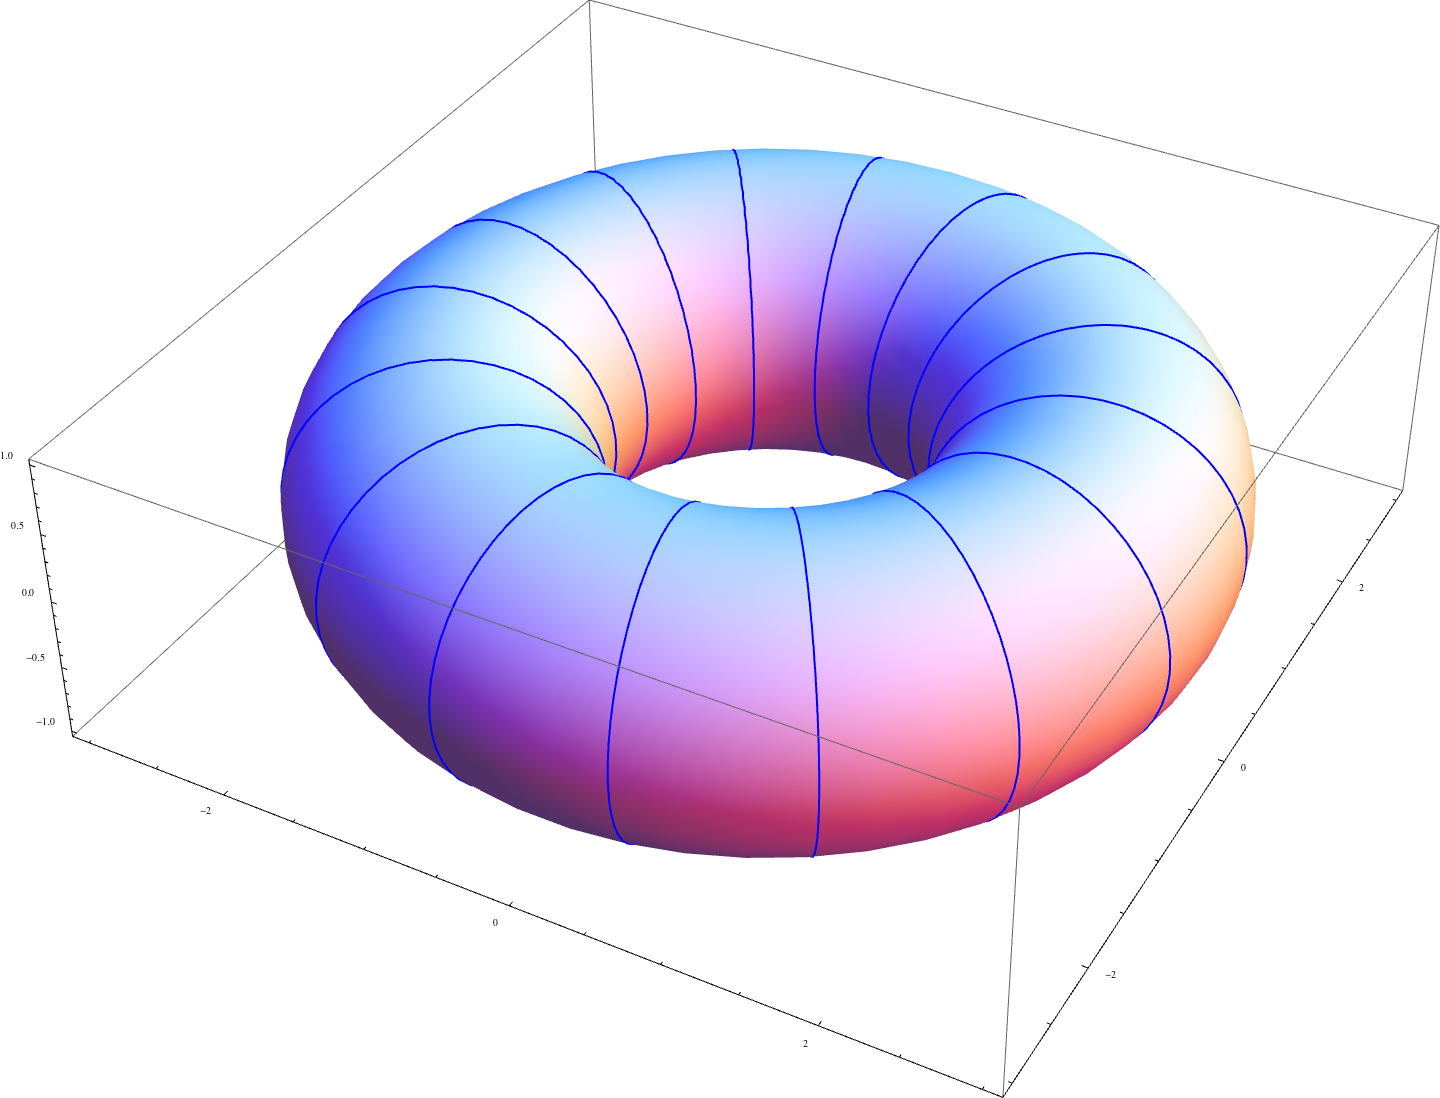
\includegraphics[width=0.4\textwidth, keepaspectratio]{Mathematica/torus.png}
	\text{Torus} \qquad \begin{tikzpicture}[scale=0.7]
		\draw[very thick] (0,0) rectangle (4,4);
		\foreach \x in {0,0.5,...,4}{
			\draw[thick, arrows={-angle 90}] (\x,1.8) -- (\x,4);
			\draw[thick, arrows={-angle 90}] (\x,0) -- (\x,2);
		}
	\end{tikzpicture}
\]
$a= \sqrt{11}$ \missingfigure{Torus + Fundamentalgebiet zum zweiten}
Betrachte nun $S^2 \subset \mathds{C} \times \mathds{R}$ 2-Sphäre
% subsubsection 252 (end)

\subsubsection{Einparameterfamilie von Diffeomorphismen} % (fold)
\label{ssub:253}
Betrachte die Abbildung $\Phi_t : M \to M$, $p \mapsto \Phi (t,p)$ mit 
\begin{itemize}
	\item $\Phi_0 = \id_M$
	\item $\Phi_s \circ  \Phi_t = \Phi_{s+t}$
\end{itemize}
Daraus folgt $\enbrace*{\Phi_t} ^{-1} = \Phi_{-t}$. Eine differenzierbare Abbildung $\Phi : \mathds{R} \times M \to M$ ist ein dynamisches System, falls
\[
	(\mathds{R},+) \to \enbrace*{ \set{\text{Diffeomorphismen auf }M}, \circ  } \quad , t \mapsto \Phi(t, .) 
\]
ein Gruppenhomomorphismus ist.
% subsubsection 253 (end)

\subsubsection{Nach $M$ parametrisierte Kurvenscharen} % (fold)
\label{ssub:254}
\[
	\gamma_p : \mathds{R} \to M \quad , \quad t \mapsto \Phi (t,p)
\]
$\gamma_p$ heißt \Index{Flusslinie}, \Index{Integralkurve}, \Index{Lösungskurve}. $\gamma(\mathds{R})$ heißt \Index{Orbit} oder \Index{Bahn} durch $p$.  
% subsubsection 254 (end)

\subsubsection[Bemerkung: Zerlegung von $M$ in ihre Bahnen]{Bemerkung} % (fold)
\label{ssub:255}
Ein dynamisches System zerlegt eine Mannigfaltigkeit disjunkt in ihre Bahnen:
\[
	q \sim p :\Leftrightarrow q= \gamma_p(t) \text{ für ein } t
\]
Die Bahnen entsprechen genau den Äquivalenzklassen.
% subsubsection 255 (end)

\subsubsection[Notation: Derivation definiert durch eine Kurve]{Notation} % (fold)
\label{ssub:256}
\[
	\vcenter{\hbox{\begin{tikzpicture}
		\draw[->] (0,0) -- (4,0) node[below right]{$\mathds{R}$};
		\draw[very thick,DodgerBlue2, ->] (1,0) node[above right]{$\diff{}{t} \in T_s \mathds{R} $}-- (2,0);
		\draw[fill, Tomato3] (1,0) circle[radius=0.03] node[below]{$s$};
		\node[right]  at (0,-0.5) {$t \mapsto t$};
	\end{tikzpicture}}} \quad \xrightarrow{\makebox[1cm]{$\gamma$}} \quad 
	\vcenter{\hbox{\begin{tikzpicture}[scale=1.3]
		%\draw[help lines] (0,0) grid (6,3);
		\coordinate (x) at (2.6,0.7);
		\coordinate (a) at (2.6,1.7);
		\coordinate (b) at (3.6,0.7);
		\draw (0,0) arc (105:70:7) node[above right, xshift=0.2cm]{$M$} arc (150:110:2.5) arc (70:105:7) arc (110:150:2.5) -- cycle;
		\draw[very thick, Tomato2] (1,0.5) to[out=20, in=180] (x) to[out=0, in=155]  (4,0.42) node[right]{$\gamma$};
		\draw[thick, SeaGreen3, shift=(x), fill=SeaGreen2!50, fill opacity=0.4] (1,0,1) -- ++ (0,0,-2)  -- ++ (-2,0,0) -- ++ (0,0,2) -- cycle;
		\node[below right, SeaGreen4] (A) at (3.6,0.7,-1) {$T_p M$} ;
		\draw[->, very thick, DodgerBlue2] (x) -- (3.4,0.7);
		\draw[fill=Firebrick3, Firebrick3] (x) circle[radius=0.025] node[below]{$p=\gamma(s)$};
	\end{tikzpicture}}}
\]
$\dot{\gamma}(s)$ steht für die Derivation, die durch $\dot{\gamma}(s) (\varphi) = \diffd{}{t}( \varphi \circ \gamma) (s) $ , $\varphi \in C^\infty(M)$ gegeben ist.
Es gilt $\dot{\gamma}(s) = T_s \gamma\enbrace*{\diff{}{t} } $. \hfill (mehr auf Blatt 6)
% subsubsection 256 (end)

\subsubsection[Satz 11: Eigenschaften von Flusslinien]{Satz 11} % (fold)
\label{ssub:257}
Eine Flusslinie eines dynamischen Systems $\gamma = \gamma_p : \mathds{R} \to M$ ist 
\begin{itemize}
	\item entweder \Index{konstant}, d.h. $\gamma(t)=p \enspace \forall t$ oder \Index{regulär}, d.h. $\dot{\gamma}(t) \not= 0 \enspace \forall t$
	\item entweder injektiv oder \Index{periodisch}, d.h. $\exists \pi \in \mathds{R}\setminus \set{0} $ mit $\gamma(t)= \gamma(t+ \pi ) \enspace \forall t$  
\end{itemize}
\minisec{Beweis}
($\gamma= \gamma_p$) Es gilt
\[
	\gamma(s+t) = \Phi_{s+t} (p) = \Phi_s \enbrace[\big]{\Phi_t (p)} = \Phi_s \enbrace[\big]{\gamma(t)}  
\]
Also 
\begin{align*}
	\dot{\gamma}(s) = T_0 \gamma(s + .) \enbrace*{\diff{}{t}} = T_0 \enbrace*{\Phi_s \circ \gamma} \enbrace*{\diff{}{t}} &= T_{\gamma(0)} \Phi \circ T_0 \gamma 
	\enbrace*{\diff{}{t} }    \\
	&= T_{\gamma(0)} \Phi_s \enbrace[\big]{\dot{\gamma}(0)} 	
\end{align*}
Da $\Phi_s$ ein Diffeomorphismus ist, gilt entweder $\dot{\gamma}(t) = 0 \enspace \forall t$ oder $\dot{\gamma}(t) \not= 0 \enspace \forall t$. Ist $\gamma$ \emph{nicht} 
injektiv, so gibt es $r < s$ mit $\gamma(r)= \gamma(s)$, d.h. $\Phi_r(p)= \Phi_s(p)$, also 
\[
	\gamma(t)= \Phi_t(p) = \Phi_{t+s-r} (p) = \gamma \enbrace[\big]{t + (s-r)} \quad \forall t \bewende 
\]
Sei $U \subseteq M$ offen. Die Flusslinien brauchen \emph{nicht} ganz in $U$ zu verlaufen! Da $\Phi ^{-1}(U)$ offen in $\mathds{R} \times M$ ist, verlaufen die Flusslinien
$\gamma_p$, $p \in U$ wenigstens für ein kleines Intervall $(a_p,b_p)$ um $0 \in \mathds{R}$.
% subsubsection 257 (end)

\subsubsection[Definition: lokaler Fluss]{Definition} % (fold)
\label{ssub:258}
Ein \Index{lokaler Fluss} auf $M$ ist eine differenzierbare Abbildung $\Phi  : D \to M$, definiert auf einer $\set{0} \times M$ enthaltener offenen Teilmenge von
$D \subset \mathds{R} \times M$, sodass für jeden Punkt $p \in M$ die Menge $D \cap (\mathds{R} \times \set{p})$ ein Intervall ist. Weiter gelte $\Phi(0,p) = p$ und 
$\Phi(s+t, p) = \Phi\enbrace[\big]{s, \Phi(t,p)}$ für alle $s,t,p$, für die beide Seiten erklärt sind.\\
Auf ${\color{Tomato2}\set{t}\times M}$ ist $\Phi_t$ kein Diffeomorphismus auf $M$, da $\Phi_t$ \emph{nicht} überall erklärt ist.
\begin{figure}[H]
	\centering{
	\begin{tikzpicture}[scale=0.7, yscale=0.9]
		\coordinate (A) at (-3,-4);
		\coordinate (B) at (3,-4);
		\coordinate (C) at (0.3,4);
		\coordinate (D) at (-2.7,4);
		%\draw[help lines] (-4,-4) grid (4,4);
		\draw[->] (-4,0) -- (4,0) node[right]{$\mathds{R} \times \set{p}$};
		\draw[->] (0,-4) node[below]{$\set{0} \times M$}-- (0,4);
		\begin{scope}
			\clip (A) -- (B) to[out=145,in=271] (C) -- (D) to[out=-30,in=50] cycle;
			\foreach \y in {-3.75,-3.5,...,3.75}{
				\draw[dashed,Chartreuse3!80] (-4,\y) -- (4,\y);
			}
		\end{scope}
		\draw[Chartreuse3, thick] (B) to[out=145,in=271] (C);
		\draw[Chartreuse3, thick] (D) to[out=-30,in=50] (A);
		\draw[Tomato2, very thick] (2,-4) -- (2,4) node[right]{$\set{t}\times M$};
		\node[Chartreuse3, below] at (-1.8,3) {$D$};
	\end{tikzpicture}
	\caption{Veranschaulichung zu lokalen Flüssen}}
\end{figure}


\minisec{Bemerkung}
\begin{itemize}
	\item Gilt $D=\mathds{R} \times M$, so ist $\Phi $ ein globaler Fluss.
	\item \begin{minipage}[t]{0.7\textwidth}
		Das Vektorfeld $\dot{\Phi}$ gegeben durch $p \mapsto X_{\gamma(p)} \equiv \dot{\gamma}(0)$ ist das \Index{Geschwindigkeitsfeld} des Flusses $\Phi$. Da 
			\[
				q= \gamma_p(t) \Rightarrow  \gamma_q(s)= \gamma_p(s+t) \Rightarrow \dot{\gamma}_q(0) = \dot{\gamma}_p(t)
			\]
			gilt $\dot{\gamma}_p(t)= \dot{\gamma}_q(0) = \dot{\Phi}_{\gamma_q(0)}$ für alle $t \in (a_p, b_p)$. (Und nicht nur für $t=0$ wie in der Definition angegeben.)
	\end{minipage}
	\begin{minipage}[b]{0.3\textwidth}
		\begin{tikzpicture}[scale=0.9, baseline=(Q)]
			\coordinate (P) at (0,0);
			\coordinate (Q) at (1,3);
			\coordinate (A) at (20:3);
			\path (Q) ++ (185:2) coordinate (B);
			%\draw[help lines] (0,0) grid (2,4);
			\draw[very thick, IndianRed3] (P) .. controls (A) and (B) .. (Q) to[out=5, in=140] ++ (-15:1) node[below]{$\gamma$};
			\draw[->, very thick,SpringGreen4] (P) -- ++ (20:1.5) node[below]{$\dot{\Phi}_p$};
			\draw[->, very thick,SpringGreen4] (Q) -- ++ (5:1.1) node[right]{$\dot{\Phi}_q$};
			\draw[fill, DodgerBlue3] (P) circle[radius=0.03] node[below]{$p$};
			\draw[fill, DodgerBlue3] (Q) circle[radius=0.03] node[above]{$q=\gamma_p(t)$};
		\end{tikzpicture}
	\end{minipage}
	\item Der Fluss eines Vektorfeldes ist ein (lokaler) Fluss. Zwei Flusslinien $\gamma_{p}^1 : I_1 \to M$ und $\gamma_p^2 : I_2 \to M$, die durch 
	$\gamma_p^1(0)= p = \gamma_p^2(0)$ verlaufen, stimmen auf $I_1 \cap I_2$ überein. Dies gilt, da aus Stetigkeitsgründen die Menge aller $t$, auf der beide Lösungen 
	übereinstimmen, abgeschlossen ist. Nach dem Satz von Picard-Lindelöf ist sie auch offen. Auf der Vereinigung aller Definitionsbereiche aller Lösungskurven $\gamma_p$
	ist die eindeutig bestimmte \Index{maximale} Lösungskurve gegeben. Wir wollen mit $D$ stets den maximalen Definitionsbereich eines Flusses angeben, d.h. es gelte stets
	\(
		D \cap (\mathds{R} \times \set{p})
	\) ist das maximale Definitionsintervall der maximalen Lösungskurve. \missingfigure{fehlende Grafik: Zusammensetzen von Flusslinien}
\end{itemize}
% subsubsection 258 (end)

\subsubsection[Beispiel: Lokaler Fluss in $\mathds{R}$]{Beispiel} % (fold)
\label{ssub:259}
Betrachte die Mannigfaltigkeit $\mathds{R}$ mit dem Vektorfeld $x^2 \diff{}{x}$. Dann ist $\Phi (t,x) = \frac{x}{1- tx}$ ein lokaler Fluss. Es gilt
\[
	\begin{cases}
		\Phi (0,x) = x \\
		\dot{\Phi}(t,x) = - \frac{(-x) x}{(1-tx)^2} = \enbrace*{\frac{x}{1-tx} }^2 \diff{}{x} = \enbrace[\big]{\Phi(t,x)}^2 \diff{}{x}     
	\end{cases}
\]
$\gamma_1(t)= \Phi(t,1)= \frac{1}{1-t} $
\[
	\begin{tikzpicture}[scale=0.7]
		%\draw[help lines] (-3,-3) grid (3,3);
		\draw[->] (-3,0) -- (3,0) node[right]{$t$};
		\draw[->] (0,-3) node[below]{$M=\mathds{R}$} -- (0,3);
		\draw[variable=\t, domain=-3:0.65, very thick, smooth] plot ({\t}, {1 /(1-\t)});
		\draw[variable=\t, domain=-0.65:3, very thick, smooth] plot ({\t}, {-1 /(1+\t)});
		\node[left] at (-3,0.5) {$\gamma_1(t)= \frac{1}{1-t} $};
		\node[right] at(3,-0.5) {$\gamma_{-1}(t)= -\frac{1}{1+t}$};
		\draw[dashed, Sienna2, thick] (-1,-3) -- (-1,3) node[below left]{$-1$};
		\draw[dashed, Sienna2, thick] (1,-3) -- (1,3) node[below right]{$1$};
	\end{tikzpicture} \qquad \quad 
	\begin{tikzpicture}[scale=0.7]
		\draw[variable=\t, very thin, fill, DarkOliveGreen3!50, smooth] plot[domain=0.333:3] (\t, 1/\t) -- (3,-3) -- plot[domain=-0.333:-3] (\t, 1/\t) -- (-3,3) -- cycle;
		\draw[variable=\t, very thick, smooth] plot[domain=0.333:3] (\t, 1/\t)  plot[domain=-0.333:-3] (\t, 1/\t) ;
		\draw[->] (-3,0) -- (3,0) node[right]{$t$};
		\draw[->] (0,-3) node[below]{$M=\mathds{R}$} -- (0,3);
		\node[DarkOliveGreen4] at (-1,1) {$D$};
	\end{tikzpicture}
\]
Definitionsbereich: $1-tx = 0 \Leftrightarrow x = \frac{1}{t}$ 
\minisec{Bemerkung}
Enthält $D$ eine Teilmenge der Form $(-\varepsilon, \varepsilon) \times M$, dann auch eine Teilmenge der Form $(-2 \varepsilon, 2 \varepsilon) \times M$.
$\Phi $ kann auf $(-2 \varepsilon, 2 \varepsilon) \times M$ durch
\[
	\Phi(t,p) := \Phi \enbrace*{\frac{t}{2}, \Phi \enbrace*{\frac{t}{2}, p }  } 
\]
ausgedehnt werden. Da $D$ maximal ist, enthält $D$ also $\mathds{R} \times M$, d.h. $\Phi $ ist global (vollständig). Dies ist beispielsweise der Fall, wenn der Träger 
$\overline{\set{X \not= 0}}$ des $\Phi$ erzeugenden Vektorfeldes $X$ kompakt ist. (Beispiel: $M$ kompakt) \\
Analog sieht man, dass jedes auf $\mathds{R}^n$ definierte und beschränkte Vektorfeld global integrierbar ist. (Blatt 7)
% subsection 259 (end)

\subsubsection[Satz 12: Jedes Vektorfeld ist Geschwindigkeitsfeld genau eines maximalen Flusses]{Satz 12} % (fold)
\label{ssub:2510}
Jedes Vektorfeld ist Geschwindigkeitsfeld genau eines maximalen Flusses.
\minisec{Beweis}
Sei $X$ ein Vektorfeld auf $M$, $\Phi $ der zugehörige Fluss (lokal). Sei $p \in M$ und $(a_p, b_p)$ maximales Definitionsintervall der Lösungskurve $\gamma_P$.
Dann ist $D = \bigcup_{p \in M} (a_p, b_p) \times \set{p}$. Es reicht zu zeigen: $D$ ist offen und $\Phi : D \to M$ ist differenzierbar.

Sei $I_p \subset [0,\infty)$ ein Intervall bestehend aus allen $t>0$, sodass $D$ eine Umgebung von $[0,t] \times \set{p}$ enthält, auf der $\Phi $ differenzierbar ist.
\begin{figure}[H]
	\centering{
	\begin{tikzpicture}[scale=1]
		% \draw[help lines] (-2,0) grid (2,4);
		\coordinate (0p) at (0,0.7) ;
		\coordinate (tp) at (0.8,0.7) ;
		\draw[very thick] (0,0) -- (0,4) node[below right]{$D$};
		\draw[thick] (-1.6,4) .. controls +(-50:1.3) and +(65:1) .. (-2,0);
		\draw[thick] (0.6,4) .. controls +(-85:1.3) and +(120:1) .. (1.5,0);
		\draw[thick, dashed, gray!70] (0,1.4) .. controls +(185:0.5) and +(80:0.4) .. (-1,0.8) .. controls +(260:0.3) and +(170:0.4) .. (-0.6,0.1)
		.. controls +(-10:0.4) and +(185:0.3) .. (0.45,0.35) .. controls +(5:0.3) and +(-90:0.4) ..(1,0.8) .. controls +(90:0.4) and +(5:0.6) .. cycle;
		\draw[thick, darkgray] (0p) node[below left]{\scriptsize $(0,p)$} -- (tp) node[below]{\scriptsize $(t,p)$};
		\foreach \b in {0p, tp} {
			\draw[fill=Tomato1] (\b) circle[radius=0.04];
		}
		\draw (0.5,1) -- (2,2) node[right]{Hier ist $\Phi$  differenzierbar};
	\end{tikzpicture}
	\caption[Das Intervall $I_p$ aus Satz 12 (\ref{ssub:2510})]{Das Intervall $I_p$, das in einer Umgebung liegt, in der $\Phi$ differenzierbar ist}}
\end{figure}
$\Rightarrow I_p$ ist offen.  
\begin{description}
	\item[$I_p$ ist \emph{nicht} leer:] Für jeden Punkt $p \in M$ gibt es $\varepsilon >0$ und eine Umgebung $U$ von $p$, sodass 
	\[
		\Phi  : (-\varepsilon, \varepsilon)\times U \to M
	\]
	differenzierbar ist. Wegen der Eindeutigkeit enthält $D$ eine Umgebung von $\set{0} \times M $ auf der $\Phi$ differenzierbar ist $\Rightarrow $ $I_p \not= \emptyset$.
	\item[$I_p$ ist abgeschlossen:] Sei $t_0$ Häufungspunkt von $I_p$ in $[0,b_p)$. Sei $q := \gamma_p(t_0)$. Nach Definition von $I_p$ gibt es eine Umgebung $V$ von $p$,
	$\varepsilon >0$ mit $t_0- 2 \varepsilon >0$, sodass $D$ eine Umgebung von $[0,t_0-\varepsilon] \times U$ enthält, auf der $\Phi$ erklärt und differenzierbar ist.
	Dabei ist $U$ eine Umgebung von $q$, sodass (für ein eventuell kleineres $\varepsilon>0$) $\Phi $ auf $(t_0 - 2 \varepsilon, t_0 + 2 \varepsilon) \times U$ definiert
	und differenzierbar ist.
	\todo[noline]{Zeichnung vervollständigen}
	\[
		\begin{tikzpicture}
			\draw[->] (-0.2,0) -- (4,0) node[right]{$t$};
			\draw[->] (0,-0.2) -- (0,2) node[left]{$M$};
		\end{tikzpicture}
	\]
	Setze: $W := \Phi_{-(t_0-\varepsilon)} \enbrace*{\Phi _{-\varepsilon} (U)} $. Also ist $\Phi$ in einer Umgebung von 
	$[0,t_0+\varepsilon] \times W \supset [0,t_0] \times \set{p}$ erklärt und differenzierbar, wenn die Abbildung 
	\[
		(t_0 - 2 \varepsilon, t_0 + 2 \varepsilon) \times  W \to M \qquad (t,r) \mapsto \Phi  \enbrace*{t-t_0, \Phi(t_0,r)} 
	\]
	setzt aufgrund der Eindeutigkeit die auf $[0,t_0 -\varepsilon] \times W$ durch $\Phi $ gegebene Lösungskurven richtig fort. Damit folgt $t_0 \in I_p$ und somit ist
	$I_p$ abgeschlossen. Argumentiert man für $(a_p,0]$ analog, so folgt $I_p = (a_p, b_p)$. \bewende
\end{description}
% subsubsection 2510 (end)
% subsection 25 (end)
% section 2 (end)
\newpage

\section{Teilung der Eins} % (fold)
\label{sec:3}
\minisec{Ziel}
Konstruktion globaler Objekte aus lokalen Daten.

\subsection{Parakompaktheit} % (fold)
\label{sub:31}
Wir setzen für $r \in \mathds{R}_{\ge0}$
\[
	C(r) := \text{ offener Würfel der Kantenlänge }2r = \set[x \in \mathds{R}^m]{\abs*{x_1}, \ldots , \abs*{x_m} < r  } 
\]
\subsubsection[Satz 13: Differenzierbare Mannigfaltigkeiten sind parakompakt]{Satz 13} % (fold)
\label{ssub:311}
Sei $\mathcal{U} = \set[U_\alpha]{\alpha \in A}$ eine offene Überdeckung einer differenzierbaren Mannigfaltigkeit $M$. Dann gibt es einen Atlas 
\[
	\mathcal{A} = \set[h_j : V_j \xrightarrow{\cong} C(3)]{j \in \mathds{N}} 
\]
von $M$, sodass 
\begin{itemize}
	\item $\set{V_j}$ ist \Index{lokal endliche Verkleinerung} von $\set{U_\alpha}$, d.h. jeder Punkt von $M$ hat eine eine Umgebung, die nur endlich viele der $V_j$
	nicht trivial schneidet, und für jedes $j$ existiert ein $\alpha(j)$ mit $V_j \subset U_{\alpha_j}$.
	\item $M = \bigcup_j h_j ^{-1}\enbrace[\big]{C(1)}$
\end{itemize}
Die Existenz einer lokal endlichen Verfeinerung zu jeder gegebenen offenen Überdeckung bezeichnet man als \Index{Parakompaktheit} des Raumes $M$. $\mathcal{A}$ heißt einer
der Überdeckung $\mathcal{U}$ \Index{untergeordneter guter Atlas}.
\minisec{Beweis}
$M$ ist \Index{lokalkompakt}\footnote{d.h. jeder Punkt hat eine kompakte Umgebung}, da $M$ lokal homöomorph zu $\mathds{R}^n$ ist. Weiter hat $M$ eine abzählbare Basis der 
Topologie\footnote{Siehe auch \ref{ssub:121}}. Daraus folgt: Es gibt eine offene Überdeckung \marginnote{Dazu kommt noch eine Übungsaufgabe}
$B_1, B_2,\ldots , B_l, \ldots $ $l\in\mathds{N}$ von $M$ mit $\overline{B}_l$ kompakt für alle $l\in \mathds{N}$.

Sei $A_1 := \overline{B}_1 $. Seien $A_1, \ldots , A_i$ induktiv konstruiert. Sei $k \in \mathds{N}$ die kleinste Zahl mit 
\[
	A_i \subset B_1 \cup \ldots \cup B_k \enspace , \quad k=k(i)
\]
Setze $A_{i+1} := \overline{B_1 \cup \ldots  \cup B_k}$. \\
(Dieser Prozess endet genau dann nach endlich vielen Schritten, wenn $M$ kompakt ist.) \smallskip \\
Nach Konstruktion gilt nun
\begin{itemize}
	\item $A_i \subset \Int(A_{i+1})$\marginnote{$\Int$ für \enquote{interior}}
	\item $A_i$ ist kompakt.
	\item $M = \bigcup_{i=1}^\infty A_i$
\end{itemize}
d.h. $\set{A_i}$ ist eine \Index{kompakte Ausschöpfung} von $M$. 
\begin{figure}[H]
	\centering{
	\begin{tikzpicture}
		%\draw[help lines] (0,-2) grid (10,2);
		\coordinate (A1) at (-1,0);
		\draw[thick] (A1) node{$A_1$} circle[radius=1];
		\foreach \p in {0,30,...,330}{
			\draw (A1) ++ (\p:1) circle[radius=0.3];
		}
		\draw[thick] (A1) circle[radius=2.3];
		\node[above left] at ($(A1)+ (300:2.3)$) {$A_2$};
		\node at (2,0) {$\cdots$};
		
		\begin{scope}
			\clip (7,0) arc (0:15:9) -- ++ (-2,0) arc(15:-15:9) -- ++ (2,0) arc(-15:0:9) -- cycle;
			\foreach \y in {-2.4, -2.2,...,2.4}{
				\draw[SteelBlue1!60, very thick] (4,\y) -- (7,\y);
			}
			%\draw[fill=green!30] (4,-2.5) rectangle (10,2.5);
		\end{scope}
		
		\foreach \r/\n in {3/-1,5/{},7/+1,9/+2}{
			\draw[thick] (\r,0) arc (0:15:9);
			\draw[thick] (\r,0) arc (0:-15:9) node[above left] {$A_{i \n}$};
		}
		
		\begin{scope}
			\clip (4,0.4) .. controls +(-75:0.5) and +(150:1) .. (5.7,-0.4) .. controls +(-30:1) and +(225:1) .. (7.4,-0.6) 
			.. controls +(45:0.5) and +(-90:0.6) .. (8,0.7) .. controls +(90:0.7) and +(-5:1) .. (6.3,1.7) 
			.. controls +(175:0.5) and +(20:0.6) .. (5.4,0.8) .. controls +(200:0.6) and +(105:0.5) .. cycle;
			\foreach \x in {2,2.25,...,7}{
				\draw[Sienna1!70, very thick, opacity=0.6] (\x,-1) -- ++ (3,3);
			}
		\end{scope}
		
		\draw[thick] (4,0.4) .. controls +(-75:0.5) and +(150:1) .. (5.7,-0.4) .. controls +(-30:1) and +(225:1) .. (7.4,-0.6) 
		.. controls +(45:0.5) and +(-90:0.6) .. (8,0.7) node[left]{$U_\alpha$} .. controls +(90:0.7) and +(-5:1) .. (6.3,1.7) 
		.. controls +(175:0.5) and +(20:0.6) .. (5.4,0.8) .. controls +(200:0.6) and +(105:0.5) .. cycle;
	\end{tikzpicture}
	\caption{Konstruktion in Satz 13 (\ref{ssub:311})}}
\end{figure}
$\Int(A_{i+1}) \setminus A_{i-1}$ ist offene Überdeckung der kompakten Menge $A_{i+1} \setminus \Int(A_{i})$. Also gibt es endlich viele Karten $h_j : V_j \xrightarrow{\cong} C(3) $, $j= j(i)$, sodass 
\begin{itemize}
	\item $V_i \subset \Int_{A_{i+2}} \setminus A_{i-1}$
	\item die $h_j ^{-1}\enbrace[\big]{C(1)}$ überdecken $A_{i+1} \setminus \Int(A_i)$
	\item $V_j \subset U_\alpha$ für ein geeignetes $\alpha$.
\end{itemize}
Man erhält also abzählbar viele Mengen $V_j$. Jede kompakte Umgebung eines Punktes ist für hinreichend großes $i$ in einem $A_i$ enthalten. Daher schneiden nur endlich 
viele der $V_j$ diese Umgebung. \bewende
% subsubsection 311 (end)

\subsubsection[Definition: Untergeordnete Teilung der Eins]{Definition} % (fold)
\label{ssub:312}
Eine $\mathcal{U}$ \Index{untergeordnete Teilung der Eins} ist eine Familie $\set[\varphi_i : M \xrightarrow{C^\infty} \mathds{R}]{i \in I} $ differenzierbarer Funktionen
mit:
\begin{itemize}
	\item Das Mengensystem der \Index{Träger} $\set[\supp \varphi_i]{i \in I} $ ist lokal endlich, wobei $\supp \varphi := \overline{\set[p \in M]{\varphi(p) \not= 0}}$.
	\item $\forall i : \exists \alpha : \supp \varphi_i \subset U_\alpha$
	\item $\varphi_i \ge 0$ und $\sum_{i \in I} \varphi_i(p) = 1 \enspace \forall p \in M$. Die Summe ist endlich, da $\set{\supp \varphi_i}$ lokal endlich ist.
\end{itemize}
% subsubsection 312 (end)

\subsubsection{Lemma 13b} % (fold)
\label{ssub:313}
Es gibt eine offene Überdeckung $B_1, B_2, \ldots , B_l , \ldots $ $l \in \mathds{N}$ von $M$ mit $\overline{B}_l$ kompakt für alle $l$.
\minisec{Beweis}
Für jeden Punkt $p \in M$ wählen wir eine Karte $(h_p,U_p)$ mit $p \in U_p$. Für $\varepsilon_p >0$ so klein gewählt, dass 
\(
	\overline{B_{\varepsilon_p}(0)} \subset h_p(U_p)
\)
setzen wir 
\[
	\Omega_p := h_p ^{-1} \enbrace*{B_{\varepsilon_p}(0)}.
\]
$\set{\Omega_p}_{p \in M}$ ist eine offene Überdeckung vom $M$, so dass $\overline{\Omega_p}$ kompakt in $M$ ist. Da $M$ eine abzählbare Basis der Topologie hat, gibt es 
eine offene Überdeckung $\set{B_l}_{l \in \mathds{N}}$ mit:
\begin{itemize}
	\item $\forall l \in \mathds{N} : \exists p=p(l) : B_l \subset \Omega_p$. Damit ist insbesondere $\overline{B}_l$ kompakt.
	\item $\Omega_p = \bigcup_{\substack{l \in \mathds{N} \\ B_l \subset \Omega_p}} B_l$. Damit ist $B_l$ a posteriori eine Überdeckung. \bewende
\end{itemize}
% subsubsection 312b (end)

\subsubsection{Satz 14} % (fold)
\label{ssub:314}
Zu jeder offenen Überdeckung $\mathcal{U}$ von $M$ gibt es eine abzählbare untergeordnete Teilung der Eins.
\minisec{Beweis}
Es gibt eine differenzierbare Funktion $\psi$ auf $\mathds{R}^m$, sodass 
\begin{itemize}
	\item $\psi \ge 0$, $\psi \le 1$,
	\item $\psi =1$ auf $\overline{C(1)}$,
	\item $\psi =0$ auf $\mathds{R}^m \setminus C(2)$
\end{itemize}
Betrachte:\\
\begin{minipage}{0.5\textwidth}
	\[
		f(t) := \begin{cases}
			e^{-\frac{1}{t} }, &\text{ falls }t >0\\
			0 , &\text{ falls } t \le 0
		\end{cases}
	\]	
\end{minipage}
\begin{minipage}{0.5\textwidth}
	\captionsetup{type=figure, skip=4pt}
	\centering{\begin{tikzpicture}[xscale=0.3, yscale=1.4]
		\draw[<->] (0,1.2) -- (0,1) node[left]{$1$} -- (0,0) -- (10,0);
		\draw[variable=\t, domain=0.0001:10, smooth, samples=50, Sienna2, very thick] plot({\t}, {exp(-1/\t)}) node[right]{$f$}; 
		\draw[dashed] (0,1) -- (10,1);
	\end{tikzpicture}
	\caption{Funktion $f$ aus \ref{ssub:313}}}
\end{minipage} \medskip\\
\begin{minipage}{0.5\textwidth}
	\[
		g(t) := \frac{f(t)}{f(t)+ f(1-t)} \enspace 
	\]
\end{minipage}
\begin{minipage}{0.5\textwidth}
	\captionsetup{type=figure, skip=4pt}
	\centering{
	\begin{tikzpicture}[xscale=1.5, yscale=1.4]
		\draw[<->] (0,1.2) -- (0,1) node[left]{$1$} -- (0,0) -- (2,0);
		\draw[variable=\t, domain=0.0001:1, smooth, samples=50, SeaGreen3, very thick] plot({\t}, {exp(-1/\t)/(exp(-1/\t) + exp(-1/(1-\t)) )}) 
		-- (2,1) node[right]{$g$}; 
		\draw[dashed] (1,0) node[below]{$1$}-- (1,1);
	\end{tikzpicture}
	\caption{Funktion $g$ aus \ref{ssub:313}}
	}
\end{minipage} \medskip\\
\begin{minipage}{0.5\textwidth}
	\[
		h(t) := g(t+2) g(2-t) \enspace
	\]
\end{minipage}
\begin{minipage}{0.5\textwidth}
	\captionsetup{type=figure, skip=4pt}
	\centering{
	\begin{tikzpicture}[xscale=1.4, yscale=1.4, domain=-2:2]
		% \draw[<->] (0,1.2) -- (0,1) node[left]{$1$} -- (0,0) -- (2,0);
		% \draw plot[id=blub] function{exp(-4/(-4+ x*x)) /((exp(1/(t+2)) + exp(-1/(t+1)))*(exp(1/(2-t)) + exp(1/(t-1)) ))} 
% 		node[right]{$h$}; 
		% \draw[variable=\t, domain=-1.9:-1.01, smooth, SeaGreen3, very thick] plot({\t}, 
		% {exp(-1/(\t+2))/(exp(-1/(\t+2)) + exp(-1/(1-(\t+2)))) * exp(-1/(2-\t))/(exp(-1/(2-\t)) + exp(-1/(1-(2-\t))))}) 
		% node[right]{$h$};
		% \draw[variable=\t, domain=-0.99:-0.01, smooth, SeaGreen3, very thick] plot({\t}, 
		% {exp(-1/(\t+2))/(exp(-1/(\t+2)) + exp(-1/(1-(\t+2)))) * exp(-1/(2-\t))/(exp(-1/(2-\t)) + exp(-1/(1-(2-\t))))}) 
		% node[right]{$h$}; 
		
		% \draw[dashed] (1,0) node[below]{$1$}-- (1,1);
		\begin{axis}[hide x axis, hide y axis, x=1cm, y=1cm, ymin=-0.5, ymax=1.5]
			\draw[<-] (axis cs: 0,1.2) -- (axis cs: 0,1) node[above left]{\footnotesize$1$} -- (axis cs: 0,0);
			\draw[->] (axis cs: -2.2,0) -- (axis cs: -2,0) -- (axis cs: 2,0) -- (axis cs: 2.2,0);
			\addplot[smooth, very thick,CadetBlue2] table {Mathematica/data_314.txt};
			\draw[fill] (axis cs: -2,0.1) -- (axis cs: -2,-0.1) node[below]{\footnotesize$-2$};
			\draw[fill](axis cs: 2,0.1) -- (axis cs: 2,-0.1) node[below]{\footnotesize $2$};
		\end{axis}
	\end{tikzpicture}
	\caption{Funktion $h$ aus \ref{ssub:313}}
	}
\end{minipage} \bigskip\\
Für den mehrdimensionalen Fall setze: $\psi(x) := h(\abs*{x_1}) \cdot h(\abs*{x_2} ) \cdots h(\abs*{x_m})$. Sei 
\[
	\set[h_j : V_j \xrightarrow{\cong} C(3)]{j \in \mathds{N}} 
\]
ein $\mathcal{U}$ untergeordneter guter Atlas (\hyperref[ssub:311]{Satz 13}).
\missingfigure{Zeichnung mit Umgebung auf Torusoberfläche}
Setze $\psi_j := \begin{cases}
	\psi \circ h_j, &\text{ auf }V_j\\
	0 , \text{ sonst}
\end{cases}$. Dann gilt
\[
	\varphi_j := \frac{\psi_j}{\sum_k \psi_k} \bewende
\]
% subsubsection 314 (end)
% subsection 31 (end)

\subsection{Riemannsche Metriken} % (fold)
\label{sub:32}
\subsubsection{Definition} % (fold)
\label{ssub:321}
Eine \Index{Riemannsche Metrik} auf einer differenzierbaren Mannigfaltigkeit $M$ ist eine Zuordnung eines Skalarproduktes $\sprod{.}{.}$ auf $T_pM$ zu jedem Punkt 
$p\in M$, das differenzierbar von $p$ abhängt. D.h. in jeder lokalen Karte sind die \Index{metrischen Koeffizienten} 
\[
	g_{ij}(p)= \sprod*{\diff{}{x^i} }{\diff{}{x^j} }_p 
\]
differenzierbare Funktionen in $p$.
% subsubsection 321 (end)

\subsubsection{Satz 15} % (fold)
\label{ssub:322}
Jede differenzierbare Mannigfaltigkeit besitzt eine Riemannsche Metrik.
\minisec{Beweis}
Sei $\set{(U_\alpha, h_\alpha)}$ ein Atlas von $M$ und $\set{\varphi_j}_{j \in \mathds{N}}$ eine untergeordnete Teilung der Eins. Das Standardskalarprodukt des 
$\mathds{R}^m$ induziert eine Riemannsche Metrik $\sprod*{.}{.}_\alpha$ auf allen Kartengebieten $U_\alpha$. Für jedes $j \in \mathds{N}$ wähle ein $\alpha(j)$ mit 
$\supp \varphi_j \subset U_{\alpha(j)}$. Dann ist 
\[
	\sprod*{.}{.}_p := \sum_{j} \varphi_j(p) \sprod*{.}{.}_{\alpha(j)} 
\]
eine Riemannsche Metrik auf $M$, da Symmetrie und positive Definitheit konvexe Eigenschaften sind. \bewende
% subsubsection 322 (end)
% subsection 32 (end)

\subsection{Sternförmige Gebiete} % (fold)
\label{sub:33}
\subsubsection[Definition: Sternförmiges Gebiet]{Definition} % (fold)
\label{ssub:331}
Eine Teilmenge $M$ des $\mathds{R}^n$ heißt \Index{sternförmig} (mit Zentrum $0$), falls mit jedem Punkt $x \in M$ auch die Strecke $\set[t \cdot x]{t \in [0,1]}$ in $M$
enthalten ist.  
% subsubsection 331 (end)

\subsubsection[Beispiel: Der Einheitsball ist diffeomorph zum $\mathds{R}^n$]{Beispiel} % (fold)
\label{ssub:332}
$\varphi : B_1(0) \xrightarrow{\cong} \mathds{R}^n $, 
\[
	x \longmapsto   \begin{cases}
		\tan \enbrace*{\frac{\pi }{2} \cdot \abs*{x}} \cdot \frac{x}{\abs*{x}}, &\text{ falls }x \not=0\\
		0 , &\text{ falls } x=0
	\end{cases}
\]
$\tan \enbrace*{\frac{\pi }{2} \cdot \abs*{x}} \cdot \frac{1}{\abs*{x}}$ ist Potenzreihe mit geraden Potenzen in $\abs*{x}$. Die Umkehrfunktion ist
\[
	\frac{2}{\pi } \arctan (\abs*{y}) \frac{y}{\abs*{y} } \longmapsfrom y  
\]
Es gilt
\[
	\mathds{R}^n \cong B_1^{n_1}(0) \times \ldots \times B_1^{n_k}(0)\quad , \quad \sum_{i} n_i = n
\]
% subsubsection 332 (end)

\subsubsection[Satz 16: Jede offene sternförmige Teilmenge des $\mathds{R}^n$ ist diffeomorph zu $\mathds{R}^n$.]{Satz 16} % (fold)
\label{ssub:333}
Jede offene sternförmige Teilmenge des $\mathds{R}^n$ ist diffeomorph zu $\mathds{R}^n$.
\minisec{Beweis}
$M$ offen, sternförmig, Zentrum $0$. \uline{Ziel}: Konstruiere einen Diffeomorphismus $\mathds{R}^n \to M$, der die Strahlen $\set[t \cdot x]{t \in [0,\infty)}$ auf ihren 
Durchschnitt mit $M$ abbildet. Diese Strahlen sind die Orbits des Vektorfeldes $X(x)=x$ auf $\mathds{R}^n$. \\
\uline{Idee}: Finde eine positive Funktion $f : M \to \mathds{R}$, sodass das Vektorfeld $Y = f \cdot X$ auf $M$ einen globalen Fluss definiert. Wir bilden dann die 
Orbits von $X$ auf die von $Y$ ab.
\minisec{Umparametrisierung}
Sei $\gamma$ eine Integralkurve von $X$, also $\dot{\gamma} = X(\gamma)$. $s : (a,b) \to \mathds{R}$ ist so zu bestimmen, dass gilt 
\[
	(\gamma \circ s)^\cdot (t) = \dot{\gamma} \enbrace*{s(t)} \dot{s}(t) \stackrel{!}{=} X_{(\gamma \circ s)(t)} \cdot f \enbrace*{(\gamma \circ  s)(t)}  = Y_{(\gamma \circ s)(t)}
\]
also $\gamma\circ s$ Lösung von $Y = f\cdot X$ ist. Nach dem Satz von Picard-Lindelöf existiert solch eine Lösung von $\dot{s}(t)= f\enbrace*{(\gamma\circ s)(t)}$ zumindest
lokal. Es werden dieselben Orbits mit Geschwindigkeit $\abs*{f X} $ statt $\abs*{X}$ in gleicher Richtung durchlaufen.

\uline{Genauer}: \oE: $M \supset K := \overline{B_1(0)}$. Wir suchen $g : M \to \mathds{R}$ positiv und \Index{eigentlich}, d.h. für jedes $j \in \mathds{N}$ ist 
$g ^{-1}([0,j])$ kompakt. Sei $\set{\varphi_j}_{j \in \mathds{N}}$ eine Teilung der Eins auf $M$ mit kompaktem Träger, $\supp \varphi_j$. Setze
\[
	g := \sum_{j=1}^{\infty} j \cdot \varphi_j
\]
Sei $K_{1+\delta }$ kompakte $\delta $-Umgebung von $K$, die noch in $M$ enthalten ist.
\[
	f := \begin{cases}
		1, &\text{ auf }K\\
		e^{-\sprod*{\grad g}{x}^2} , &\text{ sonst}
	\end{cases}
\]
Definiere $Y(x) := f(x) \cdot x$ für alle $x \in M \subseteq \mathds{R}^n$. Sei $\Phi $ der zugehörige (lokale) Fluss auf $M$.
\[
	\varphi : \mathds{R}^n \xrightarrow{\cong} M \quad ,\quad  x \mapsto \begin{cases}
		\Phi_{\log \abs*{x}} \enbrace*{ \frac{x}{\abs*{x}}}  , &\text{ falls }x \not= 0\\
		0 , &\text{ falls } x=0
	\end{cases}
\]
\begin{itemize}
	\item $\varphi$ ist wohldefiniert:
	\begin{itemize}
		\item auf $K$: $Y(x)=x$ mit Fluss $(t,x) \mapsto e^t \cdot x$, also $\varphi(x) = e^{\log \abs*{x}} \cdot \frac{x}{\abs*{x} } = x $
		\item $\Phi_t$ ist für alle Zeiten $t$ definiert (\oE $t>0$). Auf einer Flusslinie $\gamma$ von $Y = f \cdot X$ gilt:
		\[
			\abs*{\dot{(g \circ  \gamma)}} = \abs[\big]{ \sprod*{\grad g}{\dot{\gamma}} }  = f(x) \cdot \abs[\big]{ \sprod*{\grad g}{x} } = e^{- \sprod*{\grad g}{x}^2 }
			\cdot \abs[\big]{ \sprod*{\grad g}{x} } \le 1
		\]
		Benutzt: $\dot{\gamma} = f(\gamma) X(\gamma)= f(x)\cdot x \Big|_{\gamma}$. Daraus folgt (für alle $t$, für die $\gamma(t)$ existiert)
		\[
			\int_{0} ^{t} \abs*{\dot{(g \circ \gamma)}}(s)  \, \mathd s \le t , 
		\]
		also 
		\[
			\abs[\big]{ g \enbrace*{\gamma(t)} - g \enbrace*{\gamma(0)}  } = \abs*{ \int_{0} ^{t} \! \dot{(g \circ  \gamma)} (s)  \, \mathd s } \le t  
		\]
		Wäre $(-\infty, b)$ das maximale Lösungsintervall von $\gamma$ für ein $b \in (0,\infty)$, so 
		\[
			\abs[\big]{ g \enbrace*{\gamma(t)} - g \enbrace*{\gamma(0)} } \le b \text{ für alle } t \in (-\infty,b)
		\]
		Da $g$ eigentlich ist, verliefe $\gamma$ in einem Kompaktum $K'$. Dann gäbe es ein $\varepsilon>0$, so dass sich die Lösung $\gamma= \gamma(t)$ an jedem Punkt des 
		Orbits $\gamma \enbrace*{(-\infty, b)}$ um $\varepsilon >0$ fortsetzen ließe. Damit wäre also $b= + \infty$. \hfill (vgl. mit Bemerkung \ref{ssub:259}) \\
		Also ist $\Phi_t$ für alle Zeiten $t$ definiert, d.h. $\Phi$ ist global.
	\end{itemize}
	\item $\varphi$ ist ein Diffeomorphismus: $\varphi$ ist Komposition von 
	\[
		\mathds{R}^n \setminus \set{0} \to \mathds{R} \times S^{n-1} \quad ,\quad x \mapsto \enbrace*{ \log \abs*{x}, \frac{x}{\abs*{x} }  } \quad  e^t \cdot x \mapsfrom 
		(t,x)
	\]
	und $\psi : \mathds{R} \times S^{n-1} \to M \setminus \set{0}$, $(t,x) \mapsto \Phi_t(x)$, $\enbrace*{t(y), \frac{y}{\abs*{y} }}  \mapsfrom y$. Wegen 
	$\diff{}{t} \Phi_t(x) = Y(x) = f(x) \cdot x$ und $f>0$ ist die Funktion: $t \mapsto \abs*{\Phi_t(x)}$ streng monoton wachsend für alle $x \not= 0$. Die Umkehrfunktion
	bezeichnen wir mit $y \mapsto t(y)$. Also ist $\psi$ surjektiv. Mit einem analogen Argument sieht man, dass $\psi$ auch injektiv ist, da $M \setminus \set{0}$ disjunkt
	in die Bahnen von $\Phi$ ($\widehat{=}$ offene Strahlen) zerlegt ist, welche monoton wachsend durchlaufen werden. Dies und die Flusseigenschaft sichern, dass $\psi$
	ein Diffeomorphismus ist (Implizite-Funktionen-Theorem). \bewende
\end{itemize}
% subsection 333 (end)
% subsection 33 (end)
\subsection{Existenz globaler Flüsse} % (fold)
\label{sub:34}
Im Abschnitt \ref{sub:33} haben wir gesehen: Existiert eine Flusslinie nur für endliche Zeit, so verlässt sie jedes Kompaktum. Damit erhalten wir analog zu Satz 16 (\ref{ssub:333}) den folgenden Satz 17

\subsubsection{Satz 17} % (fold)
\label{ssub:341}
Zu jedem Vektorfeld $X$ auf einer differenzierbaren Mannigfaltigkeit $M$ gibt es ein \Index{vollständig integrables Vektorfeld} (d.h. der erzeugte Fluss ist global), dessen
Orbits mit den Orbits von $X$ übereinstimmen.
\minisec{Beweis (wie bei Satz 16)}
$g := \sum_{j=1}^{\infty} g \cdot \varphi_j$, $\set{\varphi_j}$ Teilung der Eins auf $M$. $\Rightarrow g$ ist eigentlich. Setze $f := e^{- (X g)^2} \in (0,1]$, 
$Y := f \cdot X$. Behauptung $Y$ ist vollständig integrabel. Entlang einer Flusslinie $\gamma$ von $Y$ gilt: 
\[
	\dot{(g \circ \gamma)} = T_{\gamma} g (\dot{\gamma}) = f(\gamma) \cdot (X g)_\gamma
\]
$\Rightarrow \dot{\abs*{(g \circ \gamma)} } \le 1$ 
\[
	\Rightarrow \abs*{ g \enbrace[\big]{\gamma(t)} - g \enbrace[\big]{\gamma(0)}  } \le \int_{0} ^{\abs*{t} } \abs*{\dot{(g \circ \gamma)}} \le \abs*{t}    
\]
Da $g$ eine eigentlich Abbildung ist, bliebe die Lösungskurve $\gamma$ in einem Kompaktum, falls $\gamma$ nur für endliche Zeiten existiert. Da dies \emph{nicht} möglich 
ist, ist der Fluss von $Y$ global. \bewende 
% subsubsection 341 (end)
Auf einer vollständigen Riemannschen Mannigfaltigkeit $(M,g)$ kann man die Vollständigkeit von Flüssen durch die Beschränktheit der integrierenden Vektorfelder erzwingen:
Sei
\begin{itemize}
	\item $M$ eine zusammenhängende differenzierbare Mannigfaltigkeit
	\item $g$ eine Riemannsche Metrik auf $M$
\end{itemize}
\[
	d(p,q) := \inf_{\gamma} \int_{a} ^{b} \! \abs*{\dot{\gamma}(t)}  \, \mathd t 
\]
definiert eine Metrik $d$ auf $M$, wobei das Infimum über alle stückweisen $C^1$-Kurven $\gamma$, die $p=\gamma(a)$ mit $q = \gamma(b)$ verbinden, erstreckt wird.

Nach dem Satz von Hopf-Rinow\footnote{Sollen wir anscheinend kennen: \url{https://de.wikipedia.org/wiki/Satz_von_Hopf-Rinow}} ist eien Riemannsche Mannigfaltigkeit $(M,g)$
\Index{vollständig} genau dann, wenn im metrischen Raum $(M,d)$ die abgeschlossenen und beschränkten Mengen kompakt sind. ($\Leftrightarrow (M,d)$ ist vollständig.)

\subsubsection{Satz 18} % (fold)
\label{ssub:342}
Jedes beschränkte Vektorfeld auf einer vollständigen Riemannschen Mannigfaltigkeit ist vollständig integrabel.
\minisec{Beweis}
Sei $(M,g)$ eine vollständige Riemannsche Mannigfaltigkeit, $X$ ein beschränktes Vektorfeld auf $M$, d.h. 
\[
	\exists K > 0 : \abs*{X} := \sqrt{g(X,X)} < K.   
\]
Wegen
\begin{align*}
	d \enbrace[\big]{\gamma(t), \gamma(0)} \le \int_{0} ^{\abs*{t}} \!  \abs*{\dot{\gamma}(s)}  \, \mathd s \le K \cdot \abs*{t} \tag*{da $\dot{\gamma} = X_\gamma$}
\end{align*}
und der Kompaktheit von $\overline{B_{K \cdot \abs*{t}} \enbrace[\big]{\gamma(0)} } $ kann man wie in Satz 17 (\ref{ssub:341}) argumentieren. \bewende
% subsubsection 342 (end) 
% subsection 34 (end)
% section 3 (end)
\newpage

\section{Vektorraumbündel} % (fold)
\label{sec:4}

\subsection{Das Tangentialbündel} % (fold)
\label{sub:41}
Die Gesamtheit der Tangentialräume einer $m$-dimensionalen differenzierbaren Mannigfaltigkeit hat die Struktur einer $2m$-dimensionalen Mannigfaltigkeit und die eines
sogenannten Vektorraumbündels.
\[
	TM := \bigsqcup_{p \in M} T_pM
\]
Es existiert eine Projektion $\pi : T M  \to M $, $X \mapsto p$, falls $X \in T_pM$. Betrachte den Atlas $\mathcal{A} = \set{(U_\alpha, h_\alpha)}_{\alpha \in A} $ für $M$ mit 
$h_\alpha = \enbrace*{x^1_\alpha, \ldots , x^m_\alpha}$. Wir wollen die Karten definieren, die $T M$ zu einer Mannigfaltigkeit machen:

\subsubsection[Definition: Tangentialbündel]{Definition} % (fold)
\label{ssub:411}
Setze für $\tilde{h}_\alpha : \pi ^{-1}(U_\alpha) \to \mathds{R}^{2m}= \mathds{R}^m \times \mathds{R}^m$ 
\[
	X \mapsto \enbrace[\Big]{h_\alpha \enbrace[\big]{\pi(X)}; X(x_\alpha^1), \ldots , X(x_\alpha^m)}
\]
D.h. mit $p \in U_\alpha$ und $X \in T_pM$, $h_\alpha(p)= (x^1, \ldots , x^m)$ und $X= X^i \diff{}{x^i} $ gilt:
\[
	\tilde{h}_\alpha(X) = \enbrace[\Big]{(x^1, \ldots , x^m), X^1, \ldots , X^m} 
\]
\begin{description}
	\item[Topologie auf $TM$:] Wird erzeugt von \marginnote{dadurch sind $\tilde{h}_\alpha$ und $\pi$ stetig}
	$\set[\tilde{h}_\alpha ^{-1}(U)]{U \subseteq \mathds{R}^{2m} \text{ offen}, (U_\alpha, h_\alpha) \in \mathcal{A}}$,
	d.h. die offenen Mengen von $TM$ sind genau Vereinigungen von endlichen Durchschnitten solcher Mengen. 
	\item[Atlas für $TM$:] $\tilde{\mathcal{A}} = \set[\enbrace*{\pi ^{-1}(U_\alpha), \tilde{h}_\alpha} ]{\alpha \in \mathcal{A}}$
	\item[Kartenwechsel:] Sei $y \in \mathds{R}^m$, $X= X^i \diff{}{x^i}$. Die Kartenwechsel
	\[
		\tilde{h}_\beta \circ \tilde{h}_\alpha ^{-1} \enbrace*{y; \begin{pmatrix}
			X^1 \\
			\vdots \\
			X^m
		\end{pmatrix}} = \enbrace*{h_\beta \circ h_\alpha ^{-1}; J_y \enbrace*{h_\beta \circ  h_\alpha ^{-1}} \begin{pmatrix}
			X^1 \\
			\vdots \\
			X^m
		\end{pmatrix} } 
	\]
	sind differenzierbar.
\end{description}
Die $2m$-dimensionale Mannigfaltigkeit $TM$ heißt das \Index{Tangentialbündel} von $M$. Die Abbildung $\pi : TM  \to M$ ist eine surjektive \Index{Submersion}, d.h. eine
differenzierbare Abbildung mit surjektivem Differential in jedem Punkt. Für jedes $p \in M$ ist $\pi ^{-1}(p)= T_p M$ ein $m$-dimensionaler Vektorraum. Daher ist $TM$
ein Beispiel eines sogenannten \bet{Vektorraumbündels}\index{Vektorraumbündel}.\\
Ein Vektorfeld $X$ auf einer differenzierbaren Mannigfaltigkeit ist ein \Index{Schnitt} des Tangentialbündels, d.h. eine differenzierbare Abbildung $X: M \to TM$ mit 
$\pi \circ X = \id_M$. Wir üblich schreiben wir $X_p := X(p) \in T_pM$,
\[
	X(\varphi)(p) := X_p(\varphi) \quad ,  \enspace\varphi \in C^\infty(M)
\]
$\Gamma(TM) := \set{\text{Vektorfelder auf }M}$ ist ein reeller Vektorraum und ein Modul über dem Ring $C^\infty(M)$.
% subsubsection 411 (end)
% subsection 41 (end)
\subsection{Das Kotangentialbündel} % (fold)
\label{sub:42}
Wir erinnern uns an die Definition des Dualraumes aus LA \RM{2}:
\begin{align*}
	T_p^* M := \enbrace*{T_pM}^* = \Hom\enbrace[\big]{T_pM, \mathds{R}} &= \text{ Vektorraum dual zu } T_p M  \\
	&= \text{ Vektorraum aller Linearformen (oder 1-Formen) auf } T_pM
\end{align*}
Wir setzen $T^*M := \bigsqcup_{p \in M} T_p^* M$. Sei weiter $\pi^{(*)} : T^*M \to M$ mit $\omega \mapsto p$, falls $\omega \in T_p^* M$. Ein Atlas 
$\mathcal{A} = \set[(U_\alpha, h_\alpha)]{\alpha \in A}$ definiert eine differenzierbare Struktur auf $T^*M$ analog zum Tangentialbündel:
\begin{description}
	\item[Karten:] $\tilde{h}^{(*)}_\alpha : \enbrace*{\pi^{(*)}} ^{-1} (U_\alpha) \to \mathds{R}^{2m}$, 
	\[
		\omega \mapsto \enbrace*{h_\alpha \enbrace*{\pi^{(*)}(\omega)}; \omega \enbrace*{\diff{}{x^1}}, \ldots , \omega \enbrace*{\diff{}{x^m} }   } 
	\]
	Sei $\mathd x^1, \ldots , \mathd x^m$ die zu $\diff{}{x^1}, \ldots , \diff{}{x^m}$ duale Basis definiert durch 
	$\mathd x^i \enbrace*{\diff{}{x^j} } = \delta_{ij} $ und $\omega= \omega_i \mathd x^i$. Dann ist
	\[
		\tilde{h}_\alpha^{(*)} (\omega) = \enbrace*{x^1, \ldots, x^m, \omega_1, \ldots , \omega_m} 
	\]
	\item[Kartenwechsel:] Eine differenzierbare Abbildung $f : M \to N$ induziert eine lineare Abbildung $f^* : T^*_{f(p)}N \to T^*_pM$ definiert durch 
	\[
		(f^* \omega)(X) := \omega \enbrace[\big]{T_p f(X)} \qquad  \quad \omega \in T_{f(p)}^*N, \quad X \in T_pM
	\]
	In lokalen Koordinaten ist diese Abbildung durch die Transponierte $J(f)^T$ der Jacobischen gegeben:\marginnote{siehe auch \ref{ssub:157}}
	\begin{align*}
		\enbrace*{f^*(\mathd y^j)} \enbrace*{\diff{}{x^i} } = \mathd y^j \enbrace[\bigg]{\underbrace{T f \enbrace*{\diff{}{x^i} }}_{= \diff{f^k}{x^i} \diff{}{y^k}} } 
		= \mathd y^j \enbrace*{\diff{f^k}{x^i} \diff{}{y^k}} = \diff{f^k}{x^i} \mathd y^j \enbrace*{\diff{}{y^k} } = \diff{f^j}{x^i}    
	\end{align*}
	Damit folgt $f^* \mathd y^j = \diff{f^j}{x^i} \mathd  x^i $, wobei $j$ der Zeilenindex und $i$ der Spaltenindex ist. Wie für die Kartenwechsel für $TM$ sehen wir,
	dass die Kartenwechsel von $T^*M$ in den ersten $m$-Komponenten durch die Kartenwechsel auf $M$ gegeben sind. In den zweiten $m$ Komponenten durch die Transponierte 
	der Jacobischen dieser Kartenwechsel. 
\end{description}

\subsubsection[Definition: $1$-Form]{Definition} % (fold)
\label{ssub:421}
Eine \bet{$1$-Form}\index{1-Form@$1$-Form} $\omega$ auf einer differenzierbaren Mannigfaltigkeit $M$ ist ein differenzierbarer Schnitt des Kotangentialbündels, d.h. 
$\omega \in C^\infty(M, T^*M)$ mit $\pi^{(*)} \circ \omega = \id_M$. Wir definieren wieder $\Gamma(T^*M) := \set{1 \text{-Formen auf }M}$. \smallskip \\
Sei $f \in C^\infty(M)$. Betrachte Testfunktion auf $\mathds{R}$: $\mathds{R} \ni t \xmapsto{\id} t \in \mathds{R}$. Dann gilt
\[
	T_p f (X) (\id) = X( \id \circ f) = X(f)
\]
d.h. lokal gilt $T_p f(X) = X(f) \diff{}{t}$.
% subsubsection 421 (end)

\subsubsection[Definition: Totales Differential]{Definition} % (fold)
\label{ssub:422}
Für $f \in C^\infty(M)$ sei $\mathd  f(X) := X(f)$. Also $(\mathd f)_p (X_p) = X_p f$. Dies ist das \bet{totale} oder 
\bet{äußere Differential}\index{Differential!totales/äußeres}. $\mathd f$ ist eine $1$-Form auf $M$. Seien $(x^1, \ldots , x^m)$ lokale Koordinaten, dann gilt
\[
	\mathd x^i \enbrace*{\diff{}{x^j} } = \diff{}{x^i} x^i = \delta_{ij}  \tag{nach Def. des Differentials}
\]
Ist also verträglich mit der Eigenschaft duale Basis zu sein. Insbesondere für $f \in C^\infty(M)$ lokal:
\[
	\mathd  f_p \enbrace*{\diff{}{x^i} } = \enbrace*{\diff{}{x^i} }_p (f) = \diff{f}{x^i} (p)   
\]
d.h. $\mathd  f = \diff{f}{x^i} \mathd x^i $ ist das \Index{totale Differential}. 
% subsubsection 422 (end)
% subsection 42 (end)

\subsection{Vektorraumbündel} % (fold)
\label{sub:43}
\subsubsection[Definition: Vektorraumbündel]{Definition} % (fold)
\label{ssub:431}
Ein ($n$-dimensionales reelles topologisches) \Index{Vektorraumbündel} über $B$ ist ein Tripel $(E,\pi, B)$ mit
\begin{itemize}
	\item $E,B$ sind Hausdorff-Räume. \marginnote{$B$ als Mannigfaltigkeit, $E$ als Menge der Tangentialräume vorstellen $\Rightarrow$ Tangentialbündel}
	\item $\pi : E \to B$ ist stetige Surjektion, sodass jede \Index{Faser} $E_b := \pi ^{-1}(b)$ für $b \in B$ die Struktur eines $n$-dimensionalen Vektorraumes 
	hat, und sodass
	\item \Index{lokale Trivialität} gilt: Für jedes $b \in B$ gibt es eine Umgebung $U$ von $b$ und einen Homöomorphismus $\varphi : \pi^{-1}(U) \to U\times \mathds{R}^n$,
	sodass  
	\[
		\varphi_{b'} := \varphi\big|_{E_{b'}} : E_{b'} \to \set{b'} \times \mathds{R}^n 
	\]
	ein Vektorraumisomorphismus für jedes $b' \in U$ ist.
\end{itemize}
$E$ heißt der \Index{Totalraum}, $\pi $ die \Index{Bündelprojektion}, $B$ die \Index{Basis}, $n$ der \Index{Rang} des Bündels und $(U,\varphi)$ \Index{Bündelkarte}.
\todo[noline]{Mischwesen aus Diagramm und Zeichnung vervollständigen}
\[
	\begin{tikzcd}
		\pi ^{-1}(U) \rar{\varphi} \dar{\pi}& U \times \mathds{R}^n \dlar{\mathrm{pr}_1} \\
		U &
	\end{tikzcd}
\]
Ein Bündel heißt \bet{trivial}\index{triviales Bündel}, falls es eine (globale) Bündelkarte $(B,\varphi)$ gibt, d.h. 
\[
	\varphi : E \xrightarrow{\cong} B \times \mathds{R}^n 
\]
\minisec{Beispiele}
\begin{itemize}
	\item $B \times \mathds{R}^n$ triviales Bündel
	\item $(TM, \pi, M)$, $(T^*M, \pi^{(*)}, M)$
	\item Möbiusband: \todo{Bündelstruktur im Möbiusband hervorheben}
	\(
		\vcenter{\hbox{\begin{tikzpicture}[yscale=0.4, xscale=0.8]
					\begin{axis}[
					    hide axis,
					    view={40}{40}
					]
					\addplot3 [
					    surf, shader=faceted interp,
					    point meta=x,
					    colormap/greenyellow,
					    samples=50,
					    samples y=5,
					    z buffer=sort,
					    domain=0:360,
					    y domain=-0.5:0.5
					] (
					    {(1+0.5*y*cos(x/2)))*cos(x)},
					    {(1+0.5*y*cos(x/2)))*sin(x)},
					    {0.5*y*sin(x/2)});

					\addplot3 [
					    samples=70,
					    domain=-145:180, % The domain needs to be adjusted manually, depending on the camera angle, unfortunately
					    samples y=0,
					    thick
					] (
					    {cos(x)},
					    {sin(x)},
					    {0});
					\end{axis}
		\end{tikzpicture}}} \not\cong \quad S^1 \times \mathds{R}
	\)
	\item $B= \mathds{R}P^1 = \nicefrac{S^1}{x \sim -x}$, $E = \set[{([x], \lambda x) \in \mathds{R}P^1 \times \mathds{R}^2}]{x \in S^1, \lambda \in \mathds{R}} $ 
	\Index{Kanonisches Bündel}, $\pi : E \to B$ mit $([x], \lambda x) \mapsto [x]$. Dann ist $E_{[x]}$ eine Gerade durch $x$ aufgefasst als Vektorraum.
	\begin{figure}[H]
		\centering{
		\begin{tikzpicture}
			\coordinate (x) at (35:1);
			\coordinate (-x) at (215:1);
			\coordinate (zero) at (0,0);
			\draw[thick] (0,0) node[below]{$0$} circle[radius=1] ;
			\draw[thick] (215:1.5) -- (-x) node[left]{$-x$} -- (x) node[right]{$x$}-- ++ (35:0.5);
			\foreach \b in {x,-x,zero}{
				\draw[fill=Tomato1] (\b) circle[radius=0.035];
			}
		\end{tikzpicture}
		\caption{Kanonisches Geradenbündel}}
	\end{figure}
\end{itemize}
% subsubsection 431 (end)

\subsubsection[Definition: Bündelmorphismus]{Definition} % (fold)
\label{ssub:432}
Ein \Index{Bündelmorphismus} $(E,\pi , B) \to (E', \pi', B')$  ist ein Paar $(f, \overline{f})$ stetiger Abbildungen $f : E \to E'$ und $\overline{f} : B \to B'$ mit
\(
	\overline{f} \circ \pi  = \pi' \circ f, 
\)
d.h. 
\[
	\begin{tikzcd}
		E \rar{f} \dar{\pi }& E' \dar{\pi'}\\
		B \rar{\overline{f}}& B'
	\end{tikzcd}
\]
und mit  $f_b := f\big|_{E_b} : E_{b} \to E_{\overline{f}(b) }'$ linear für alle $b \in B$.
\minisec{Bemerkung}
Da $\pi $ surjektiv ist, ist $\overline{f}$ durch $f$ und durch $\overline{f} \circ \pi = \pi' \circ f $ eindeutig festgelegt. Daher schreiben wir auch $f : E \to E'$ für
einen Bündelmorphismus.
\minisec{Beispiele}
\begin{itemize}
	\item Das Differential $T f : TM \to TN$ einer differenzierbaren Abbildung $f : M \to N$ ist ein Bündelmorphismus.
	\item Falls $f : M \xrightarrow{\cong} N$, dann ist die induzierte Abbildung $f^* : T^*N \to T^* M$, $\omega \mapsto \omega \circ Tf$ ein Bündelmorphismus.
\end{itemize}
% subsubsection 432 (end)

\subsubsection[Definition: Bündeläquivalenz]{Definition} % (fold)
\label{ssub:433}
Eine \Index{Bündeläquivalenz} ist ein Bündelmorphismus mit $B = B'$, $\overline{f} = \id_B$ und $f_b$ ein Isomorphismus für jedes $b \in B$.
\minisec{Beispiel}%
\begin{figure}[h]%
	\centering{
	\tikzsetnextfilename{induziertes_Buendel}
	\begin{tikzpicture}[scale=1.1]
		%\draw[help lines] (0,0) grid(13,8);
		\coordinate (a) at (1.5,5);
		\coordinate (b) at (3,5);
		\draw[thick] (0,5) -- (a) -- (b) -- (4,5) node[below]{$\mathds{R}$};
		\draw (a) +(0.3,1) -- +(-0.3,0.5) -- + (-0.3,-1) -- +(0.3,-0.5) -- cycle;
		\draw (b) +(0.3,1) -- +(-0.3,0.5) -- + (-0.3,-1) -- +(0.3,-0.5) -- cycle;
		\draw[->] (4.5,5) -- (5,5) node[below]{$\gamma$} -- (5.5,5);
		\draw (9,3) .. controls +(75:1) and +(190:1) .. (12,5) 
		.. controls +(110:0.5) and +(210:1) .. (13,7) 
		.. controls +(170:4) and + (85:3) .. (6,4.5) node[below right]{$M$}
		.. controls +(-5:2) and +(120:1) .. (9,3);
		\coordinate (c) at (7,5);
		\coordinate (d) at (8,5.2);
		\coordinate (e) at (10.5,6.5);
		\coordinate (f) at (8.3,6.5);
		\coordinate (g) at (11,5.5);
		\draw[thick] (6.5,5) .. controls +(0:0.1) and +(185:0.1) .. (c)
		.. controls +(5:0.3) and +(190:0.3) .. (d)
		.. controls +(10:1) and +(-40:1) .. (e)
		.. controls +(140:0.7) and +(30:0.7) .. (f)
		.. controls +(210:0.7) and +(160:0.7) .. (d)
		.. controls +(-20:1) and +(200:1) .. (g) -- +(20:0.7) node[below]{$\gamma$};
		\foreach \b in {a,...,g}{
			\draw[fill=Tomato1] (\b) circle[radius=0.045];
		}
		\draw (c) +(50:0.4) --+(140:0.4) --+(230:0.4) --+(320:0.4) -- cycle;
		\draw (d) +(25:0.4) --+(115:0.4) --+(205:0.4) --+(295:0.4) -- cycle;
		\draw (e) +(185:0.4) --+(275:0.4) --+(5:0.4) --+(95:0.4) -- cycle;
		\draw (f) +(255:0.4) --+(345:0.4) --+(75:0.4) --+(165:0.4) -- cycle;
		\draw (g) +(65:0.4) --+(155:0.4) --+(245:0.4) --+(335:0.4) -- cycle;
	\end{tikzpicture}
	\caption{Beispiel für das induzierte Bündel}}
\end{figure}%
$(E, \pi , B)$ gegebenes Bündel. $f : B_0 \to B$ stetige Abbildung. Dann gibt es ein Bündel $(f^*E, f^*\pi, B_0)$ und einen faserweisen isomorphen Bündelmorphismus
$(\tilde{f},f) : (f^*E, f^*\pi, B_0) \to (E,\pi , B)$
\[
	\begin{tikzcd}
		 f^*E \dar{f^*\pi } \rar{\tilde{f}} & E \dar{\pi} \\
		 B_0 \rar{f}& B
	\end{tikzcd}
\]
Dieses Bündel ist eindeutig bis auf Bündeläquivalenz.
\minisec{Konstruktion}
Setze
\[
	f^*E := \set[(b_0,e) \in B_0 \times E]{f(b_0) = \pi(e)} 
\]
$f^* \pi : f^*E \to B_0$, $(b_0,e) \mapsto b_0$ und $\tilde{f} : f^*E \to E$, $(b_0,e) \mapsto e$. Es gilt
\begin{align*}
	f \circ f^* \pi (b_0,e) = f(b_0) = \pi(e) = \pi \circ \tilde{f}(b_0,e),
\end{align*}
d.h. $\tilde{f}$ ist ein Bündelmorphismus, falls $f^*E$ ein Bündel ist, der faserweise isomorph ist: 
\[
	\set[(b_0,e)]{\pi(e)= f(b_0)} = (f^*E)_{b_0} \xrightarrow{\cong} E_{f(b_0)}, (b_0,e) \mapsto e 
\]
\uline{$f^*E$ ist lokal trivial:} Für einen Punkt in $B_0$ wählen wir eine Umgebung $U_0 \subset B$, sodass $f(U_0) \subset U$ für eine Bündelkarte $(U,\varphi)$ für $E$.
Das heißt $\varphi : \pi  ^{-1}(u) \xrightarrow{\cong} U \times \mathds{R}^n $ und
\[
	\varphi_b = \varphi\big|_{\pi ^{-1}(b)} : \pi  ^{-1}(b) \xrightarrow[\text{linear}]{\cong} \set{b} \times \mathds{R}^n 
\]
Wir setzen: $\varphi_0 : \pi  ^{-1} (U_0) \to U_0 \times \mathds{R}^n$, $(b_0,e) \mapsto \enbrace[\big]{b_0, \mathrm{pr}_2 \circ \varphi_{f(b_0)}(e)}$, wobei $\mathrm{pr}_2$ die Projektion auf die zweite Komponente ist. $\varphi_0$ ist faserweise isomorph. Die Inverse ist
\[
	\enbrace*{b_0, \varphi ^{-1} \enbrace[\big]{f(b_0), v} } \mapsfrom (b_0, v)
\]
\uline{Eindeutigkeit:} Sei mit $\tilde{f}_1$ faserweise isomorph
\[
	\begin{tikzcd}
		E_1 \drar{g} \arrow[ddr, swap, "\pi_1", bend right] \arrow[drr, "\tilde{f}_1", bend left]& & \\
		 & f^*E \rar{\tilde{f}} \dar{f^*\pi} & E \dar{\pi } \\
		& B_0 \rar{f} & B
	\end{tikzcd}
\]
wobei $g(e_1) = \enbrace*{\pi_1(e_1), \tilde{f}_1(e_1)} $. Das Diagramm ist kommutativ.
% subsubsection 433 (end)

\subsubsection{Produktbündel: $\xi \times \eta$} % (fold)
\label{ssub:434}
\index{Produktbündel}
\begin{align*}
	\xi & := \enbrace[\big]{E(\xi), \pi(\xi), B(\xi)} \\
	\eta & := \enbrace[\big]{E(\eta), \pi (\eta), B(\eta)}
\end{align*}
Wir setzen:
\begin{align*}
	E(\xi \times \eta) & := E(\xi) \times E(\eta) \\
	B(\xi \times \eta) & := B(\xi) \times B(\eta) \\
	\pi_{\xi \times \eta} (e,f) & := \enbrace[\big]{\pi_\xi(e), \pi_\eta(f)} 
\end{align*}
% subsubsection 434 (end)

\subsubsection{Whitney-Summe:  $\xi \oplus \eta$} % (fold)
\label{ssub:435}
Seien $\xi, \eta$ Bündel über $B$. Definiere nun die \Index{Diagonalabbildung}\index{Whitney-Summe}
\[
	\Delta : B \to B \times B \qquad b \mapsto (b,b)
\]
Setze nun $\xi \oplus \eta := \Delta^*(\xi \times \eta)$. Dann gilt $E_b(\xi \oplus \eta) = E_b(\xi) \oplus E_b(\eta)$. Weiter gilt auch
\[
	\xi \oplus \eta \cong \eta \oplus \xi \qquad , \qquad (\xi \oplus \eta) \oplus \zeta \cong \xi \oplus (\eta \oplus \zeta)
\]
% subsubsection 435 (end)

\subsubsection{Einschränkung eines Bündels} % (fold)
\label{ssub:436}
Sei $B_0 \subset B(\xi)$. Dann betrachte 
\[
	\xi\big|_{B_0} = \enbrace[\Big]{\pi ^{-1}(B_0), \pi\big|_{\pi ^{-1} (B_0)}, B_0} 
\]
Für die Inklusionsabbildung $i : B_0 \hookrightarrow B$ gilt: $i^* \xi = \xi\big|_{B_0}$ ist ein Bündel.
\minisec{Beispiel: $S^2 \subseteq \mathds{R}^3$}
\[
	\begin{tikzpicture}[scale=1.5]
		\draw (-1,0) arc (180:360:1cm and 0.5cm);
	    \draw[dashed] (-1,0) arc (180:0:1cm and 0.5cm);
	    \draw (0,1) arc (90:270:0.5cm and 1cm);
	    \draw[dashed] (0,1) arc (90:-90:0.5cm and 1cm);
	    \draw (0,0) circle (1cm);
	    \shade[ball color=blue!10!white,opacity=0.20] (0,0) circle (1cm);
	\end{tikzpicture}
\]\todo[inline]{Zeichnung vervollständigen!}
Es gibt drei Bündel: $\mathds{R}^3\big|_{S^2}$, $\mathds{R} \underline{n}$, $T S^2$. Sei $\varepsilon^k$ das triviale, $k$-dimensionale Bündel (hier über $S^2$). Es gilt
\begin{align*}
	\mathds{R}^3\big|_{S^2} &= \varepsilon^3 = S^2 \times \mathds{R}^3 \\
	\mathds{R} \underline{n} &= \varepsilon^1 = S^2 \times \mathds{R} \\
	T S^2 & \not= \varepsilon^2
\end{align*}
Nun gilt 
\[
	T S^2 \oplus \varepsilon^1 \cong T \mathds{R}^3 \big|_{S^2} \cong \varepsilon^3 \cong \varepsilon^2 \oplus \varepsilon^1
\]
% subsubsection 436 (end)

\subsubsection[Definition: Schnitt von Bündeln]{Definition} % (fold)
\label{ssub:437}
Eine stetige Abbildung $\sigma : B  \to E$ mit $\pi \circ \sigma = \id_B$ heißt \bet{Schnitt}\index{Schnitt eines Bündels} des Bündels $(E,\pi ,B)$.
\todo{Zeichnung vervollständigen!}
\[
	\begin{tikzpicture}
		%\draw[help lines] (0,0) grid(8,4);
		\coordinate (a) at (1,1.7);
		\coordinate (b) at (2,2);
		\coordinate (c) at (3,2.15);
		\coordinate (d) at (4,2.2);
		\coordinate (e) at (5,2.15);
		\coordinate (f) at (6,2);
		\coordinate (g) at (7,1.7);

		\draw[thick,DarkGoldenrod2] (0,0.5) .. controls +(20:1) and +(180:1) .. (2,2.5)
		.. controls +(0:1) and +(180:0.5) .. (4,1.5)
		.. controls +(0:1) and +(180:0.5) .. (6,2.5)
		.. controls +(0:0.5) and +(190:0.5) .. (7,1.5)
		.. controls +(10:0.5) and +(195:0.5) .. (8,1.7) node[right]{$\sigma(B)$};
				
		\draw[thick] (0,1) .. controls +(50:0.3) and +(205:0.3) .. (a)
		.. controls +(25:0.4) and +(190:0.4) .. (b)
		.. controls +(10:0.4) and +(185:0.4) .. (c)
		.. controls +(5:0.4) and +(180:0.4) .. (d)
		.. controls +(0:0.4) and +(175:0.4) .. (e)
		.. controls +(-5:0.4) and +(170:0.4) .. (f)
		.. controls +(-10:0.4) and +(155:0.4) .. (g)
		.. controls +(-25:0.3) and +(130:0.3) .. (8,1) node[right]{$E$};
		
		\draw (a) +(110:0.9) -- +(-70:0.9);
		\draw (b) +(100:0.9) -- +(-80:0.9);		
		\draw (c) +(95:0.9) -- +(-85:0.9);
		\draw (d) +(90:0.9) -- +(-90:0.9);
		\draw (e) +(85:0.9) -- +(-95:0.9);
		\draw (f) +(80:0.9) -- +(-100:0.9);
		\draw (g) +(70:0.9) -- +(-110:0.9);				
		
		\draw[->] (3.5,1) -- (3.5,0.6) node[right]{$\pi$} -- (3.5,0.2);
		\draw[->,DarkGoldenrod2] (4.5,0.2) -- (4.5,0.6) node[right]{$\sigma$} -- (4.5,1);
		
		\draw[thick] (0,0) -- (8,0) node[right]{$B$};
	\end{tikzpicture}
\] 
% subsubsection 437 (end)

\subsubsection[Definition: Bündelatlas]{Definition} % (fold)
\label{ssub:438}
Eine Menge $\set[(U_\alpha, \varphi_\alpha)]{\alpha \in A}$ von Bündelkarten für $(E,\pi ,B)$ heißt \Index{Bündelatlas}, falls $\bigcup_{\alpha \in A} U_\alpha = B$.
Die stetigen Abbildungen
\begin{gather}
	\varphi_{\alpha \beta} : U_\alpha \cap U_\beta \longrightarrow Gl(k,\mathds{R}) \quad, \qquad b \longmapsto \varphi_{\beta,b} \circ \varphi_{\alpha,b} ^{-1} \\
	 \enbrace*{ \varphi_{\alpha, b} := (\mathrm{pr}_2 \circ \varphi_\alpha)\big|_{E_b} : E_b \xrightarrow{\cong} \mathds{R}^k } 
\end{gather}
heißen \Index{Übergangsfunktionen}.
\minisec{Beispiel}
$h_\beta \circ  h_\alpha ^{-1}$ Kartenwechsel einer differenzierbaren Mannigfaltigkeit $M$. Dann ist $J_{h_\beta \circ h_\alpha ^{-1}}$ sind die Übergangsfunktionen von
$T_p M$. \medskip\\
Ein Bündelatlas eines Bündels über einer differenzierbaren Mannigfaltigkeit heißt \bet{differenzierbar}\index{Bündelatlas!differenzierbar}, falls also Übergangsfunktionen 
differenzierbar sind. Ein \bet{differenzierbares Vektorbündel}\index{Vektorbündel!differenzierbar} ist ein Vektorbündel mit einem maximalen differenzierbaren Bündelatlas.
$\Rightarrow$ Der Totalraum eines differenzierbaren $\mathds{R}^k$-Bündels über $M^m$ ist in kanonischer Weise eine $m+k$-dimensionale differenzierbare Mannigfaltigkeit.

Mittels der Übergangsfunktionen lässt sich der Totalraum $E$ auch wie folgt darstellen:
\[
	E := \frac{\bigsqcup_{\alpha \in A} U_\alpha \times \mathds{R}^k}{(x,v) \sim \enbrace*{x, \varphi_{\alpha \beta}(x) \cdot v}} 
\]
wobei $(x,v) \in U_\alpha \times \mathds{R}^k$, $x\in U_\alpha \cap U_\beta$ und $\enbrace*{x, \varphi_{\alpha \beta}(x) \cdot v} \in U_\beta \times \mathds{R}^k$
\minisec{Beispiel}
Bis auf Äquivalenz gibt es genau zwei $\mathds{R}^k$-Bündel über $S^1$, da $Gl(k,\mathds{R})$ zwei Zusammenhangskomponenten hat.\todo{Zeichnung vervollständigen}
\[
	\begin{tikzpicture}
		\draw (0,0) circle[radius=2];
	\end{tikzpicture}
\]
\minisec{Anwendung}
Whitney-Summe: Betrachte
\[
	\set{\enbrace[\big]{U_\alpha \cap V_\beta, \varphi_\alpha \oplus \psi_\beta}} 
\]
Dann gilt
\[
	E(\xi \oplus  \eta) = \frac{\bigsqcup_{\alpha,\beta} (U_\alpha \cap V_\beta) \times (\mathds{R}^k  \oplus  \mathds{R}^l)}{(x,(v,w)) \sim \enbrace*{x,
	\enbrace*{\varphi_{\alpha \alpha'}(x) \cdot v, \psi_{\beta \beta'}(x) \cdot w} } } 
\]
wobei $(x,(v,w)) \in (U_\alpha \cap V_\beta) \times (\mathds{R}^k \oplus \mathds{R}^l) $ und $\enbrace[\big]{x,\enbrace*{\varphi_{\alpha \alpha'}(x) \cdot v, 
\psi_{\beta \beta'}(x) \cdot w} } \in (U_{\alpha'} \cap V_{\beta'}) \times (\mathds{R}^k \oplus \mathds{R}^l)$. \medskip \\
Analog: $\xi \otimes  \eta$, $\xi^*$, $\Hom(\xi, \eta)$, $\eta \subseteq \xi$: $\nicefrac{\xi}{\eta}$, \ldots 
% subsubsection 438 (end)
% subsection 43 (end)
% section 4 (end)
\newpage

\section{Formen} % (fold)
\label{sec:5}

\subsection{Alternierende Formen} % (fold)
\label{sub:51}

\subsubsection[Definition: Alternierende $k$-Form]{Definition} % (fold)
\label{ssub:511}
Eine (alternierende) $k$-Form auf einem $n$-dimensionalen Vektorraum $V$ ist eine multilineare Abbildung 
\[
	\omega : \underbrace{V \times \ldots \times V}_{\text{$k$-mal}} \to \mathds{R},
\]
die in folgendem Sinne \Index{alternierend} ist: 
\[
	\forall v_1, \ldots , v_k \in V : \forall \pi \in S_k : \omega \enbrace*{v_{\pi(1)}, \ldots , v_{\pi(k)}} = \sgn(\pi )\cdot  \omega(v_1, \ldots , v_k) 
\]
Beispiel: Die Determinante als multilineare Abbildung in ihren Spalten (Zeilen) ist eine $n$-Form. $\Lambda^k V^*$ ist der reelle Vektorraum der $k$-Formen auf $V$.
Es ist $\Lambda^1 V^* = V^*$, $\Lambda^0 V^* := \mathds{R}$.
% subsubsection 511 (end)

\subsubsection[Definition: Äußeres Produkt, Dachprodukt]{Definition} % (fold)
\label{ssub:512}
Das \Index{äußere Produkt} (oder auch \Index{Dachprodukt}) zweier Formen ist eine bilineare Abbildung 
\[
	\Lambda^k V^* \times \Lambda^l V^* \to \Lambda^{k+l} V^*, \qquad (\omega, \sigma ) \mapsto \omega \wedge \sigma 
\]
das wie folgt erklärt ist: $\forall v_1, \ldots , v_{k+l} \in V :$
\[
	 (\omega \wedge \sigma)(v_1, \ldots , v_{k+l}) = \frac{1}{k! \cdot l!} \sum_{\pi \in S_{k+l}} \sgn(\pi ) \cdot \omega\enbrace*{v_{\pi(1)}, \ldots , v_{\pi(k)}} \cdot 
	 \sigma \enbrace*{v_{\pi(k+1)}, \ldots , v_{\pi(k+l)} }
\]
\minisec{Bemerkung}
Die rechte Seite ist gleich
\[
	\sum_{\pi \in S_{k+l}}' \sgn(\pi) \cdot \omega\enbrace*{v_{\pi(1)}, \ldots , v_{\pi(k)}} \cdot \sigma\enbrace*{v_{\pi(k+1)}, \ldots , v_{\pi(k+l)}}
\]
wobei die Summe über alle Permutationen mit $\pi(1) < \ldots < \pi(k)$, $\pi(k+1) < \ldots < \pi(k+l)$ erstreckt wird. In der alternierenden Summe der Definition kommen
genau diejenigen Summanden mehrfach vor, deren Permutationen gewisse Zerlegungen 
\[
	\set{1, \ldots , k+l} = \set{\pi(1), \ldots , \pi(k)} \sqcup \set{\pi(k+1), \ldots , \pi(k+l)}  
\]
erhalten. Fasst man diese in Äquivalenzklassen zusammen, in sogenannte \Index{Zerlegungen} $[\pi ] \in \mathcal{Z}_{k+l}$, so hat jede solche Klasse $k!\cdot l!$ Vertreter.
In der Summe der Bemerkung haben wir einen solchen Vertreter ausgezeichnet.

Das äußere Produkt ist assoziativ:
\[
	(\omega \wedge \sigma) \wedge \tau = \omega \wedge (\sigma \wedge \tau)
\]
Dazu betrachte man Zerlegungen aus $\mathcal{Z}_{k,l,m}$ und stellt fest, dass beide Seiten angewandt auf $(v_1, \ldots , v_{k+l+m})$ geben:
\[
	\sum_{\pi \in S_{k+l+m}}' \sgn(\pi) \cdot \omega(v_{\pi(1)}, \ldots , v_{\pi(k)}) \cdot \sigma(v_{\pi(k+1)}, \ldots , v_{\pi(k+l)}) \cdot \tau(v_{\pi(k+l+1)}, \ldots , 
	v_{\pi(k+l+m)})
\]
% subsubsection 512 (end)

\subsubsection[Lemma 20: Basis des Vektorraumes $\Lambda^k V^*$]{Lemma 20} % (fold)
\label{ssub:513}
Sei $e_1^*, \ldots , e_n^*$ eine Basis von $V^*$, dann ist 
\[
	\set[e_{i_1}^* \wedge \ldots \wedge e_{i_k}^*]{i_1 < \ldots i_k} = \set[e_I^*]{I=(i_1 < \ldots < i_k)}  
\]
eine Basis von $\Lambda^k V^*$.
\minisec{Beweis}
Sei $e_1, \ldots , e_n$ die duale Basis von $V$ ($e_i^*(e_j)= \delta_{ij}$). Sei $\omega$ eine $k$-Form. Setze 
\[
	\omega_{i_1, \ldots , i_k} := \omega \enbrace*{e_{i_1}, \ldots , e_{i_k}} 
\]
Dann gilt
\[
	\omega = \sum_{i_1 < \ldots  < i_k} \omega_{i_1, \ldots , i_k} e_{i_1}^* \wedge \ldots \wedge e_{i_k}^*
\]
$\Rightarrow $ die $e_I^*$ erzeugen $\Lambda^k V^*$. Aus $0= \sum_I' \omega_I e_I^*$ folgt durch Auswerten auf $e_{i_1}, \ldots , e_{i_k} : \omega_I = 0 \forall I$.
Also sind die $e_I^*$ linear unabhängig. \bewende \medskip \\
Also ist $\dim \Lambda^k V^* = \binom{n}{k}$.
% subsubsection 513 (end)

\subsubsection{Lemma 21 (Antikommmutativität)} % (fold)
\label{ssub:514}
Sei $\omega \in \Lambda^k V^*$, $\sigma \in \Lambda^l V^*$. Dann gilt
\[
	\omega \wedge \sigma = (-1)^{kl} \sigma \wedge \omega
\]
\minisec{Beweis}
Beide Seiten sind linear in $\omega$ und $\sigma$. Damit reicht es die Behauptung für alle Basiselemente zu zeigen. Dies folgt aus der entsprechenden Behauptung für 
$1$-Formen: $\omega \wedge \sigma = - \sigma \wedge \omega$. Dies folgt nun mit:
\begin{align*}
	\omega \wedge \sigma(v,w) = \omega(v) \cdot \sigma(w) - \omega(w) \cdot \sigma(v)
\end{align*}
ist antisymmetrisch in $\omega$ und $\sigma$. \bewende \medskip \\
Sei nun $\omega \in \Lambda^k V^*$, wobei $k$ ungerade ist. Dann ist $\omega \wedge \omega = 0$. Dies führt zu:
% subsubsection 514 (end)

\subsubsection{Lemma 22} % (fold)
\label{ssub:515}
Sind $\omega_1, \ldots , \omega_k$ $1$-Formen, so gilt $\forall v_j \in V$:
\[
	(\omega_1 \wedge \ldots \wedge \omega_k)(v_1, \ldots , v_k) = \det \enbrace[\big]{\omega_i(v_j)}
\]
\minisec{Beweis}
Beide Seiten sind multilinear und in gleicher Weise alternierend. OE: $\omega_j = e_j^*$, $v_j = e_j$. Dann gilt
\begin{align*}
	e_1^* \wedge \ldots \wedge e_k^* (e_1, \ldots , e_k) = 1 = \det (\delta_{ij}) = \det \enbrace[\big]{e_i^*(e_j)}. \bewende 
\end{align*}
$\Lambda V^* = \bigoplus_{k=0}^\infty \Lambda^k V^*$ ist, versehen mit dem äußeren Produkt, eine reelle, graduierte, assoziative, antikommutative, $2^n$-dimensionale, 
unitale Algebra, die \Index{äußere Algebra} (oder auch die \Index{Graßmann-Algebra}). \\
Betrachte nun $f : V \to W$ linear. Die \Index{induzierte Abbildung} ist eine Abbildung
\[
	f^* : \Lambda W^* \to \Lambda V^* , \qquad \omega \mapsto f^* \omega
\] 
wobei $\omega$ eine $k$-Form ist, gegeben durch
\[
	(f^* \omega)(v_1, \ldots , v_k) := \omega\enbrace[\big]{f(v_1), \ldots , f(v_k)}
\]
$f^*$ ist ein Algebrenhomomorphismus:
\[
	f^*( \omega \wedge \sigma) = (f^* \omega) \wedge (f^* \sigma)
\]
Betrachtet man nun $f : V \to V$, wobei $\dim V = n$ und eine nichttriviale $n$-Form $\omega$, d.h.
\(
	\omega \in \Lambda^n V^* \setminus \set{0} 
\)
($\dim \Lambda^n V^* = 1$), eine sogenannte \Index{Volumenform}. $\det f$ ist die eindeutig bestimmte reelle Zahl, für die gilt: $(f^* \omega) = \det(f) \cdot \omega$.
Dies hängt nicht von der Wahl der Volumenform ab! Sei $e_1, \ldots, e_n$ eine Basis von $V$, $e_1^*, \ldots , e_n^*$ die duale Basis und 
$\omega = e_1^* \wedge \ldots \wedge e_n^*$. Dann ist $f$ durch die Matrix 
\[
	A= (a_{ij}) = \benbrace*{f(e_1), \ldots , f(e_n)}
\]
gegeben. Damit:
\begin{align*}
	(f* \omega)(e_1, \ldots, e_n) = \omega \enbrace[\big]{f(e_1), \ldots , f(e_n)}  
	&= e_1^* \wedge \ldots \wedge e_n^* \enbrace*{ \sum_k a_{k1} e_k , \ldots , \sum_k a_{kn} e_k} \\
	&= \det \enbrace*{ e_i^* \enbrace*{\sum_k a_{kj} e_k}} \\
	&= \det (a_{ij}) = \det A 
\end{align*}
$\Rightarrow $ $\det f$ stimmt mit der Determinante der Matrix $A$ überein. Diese koordinatenfreie Definition wird es uns erlauben, einen Integralbegriff auf 
differenzierbaren Mannigfaltigkeiten einzuführen.
% subsubsection 515 (end)
% subsection 51 (end)

\subsection{Differentialformen} % (fold)
\label{sub:52}
\subsubsection[Definition: Differentialform]{Definition} % (fold)
\label{ssub:521}
Eine \Index{Differentialform} vom Grad $k$ (oder $k$-Form) auf einer differenzierbaren Mannigfaltigkeit $M$ ist eine Zuordnung einer $k$-Form $\omega_p$ auf $T_p M$ zu 
jedem Punkt der Mannigfaltigkeit, die differenzierbar von $p$ abhängt, d.h. in jeder lokalen Karte $(U, x^1, \ldots , x^m)$ hängen die Komponentenfunktionen
\[
	\omega_{i_1, \ldots , i_k} := \omega \enbrace*{\diff{}{x^{i_1}}, \ldots , \diff{}{x^{i_k}}} : U \longrightarrow \mathds{R} 
\]
differenzierbar von $p$ ab. Wir setzen:
\begin{align*}
	\Omega^k M &:= \text{ $\mathds{R}$-Vektorraum aller $k$-Formen auf $M$; $C^\infty(M)$-Modul} \\
	\Omega^0 M &:= C^\infty(M)
\end{align*}
% subsubsection 521 (end)

\subsubsection{Bemerkung} % (fold)
\label{ssub:522}
Das \Index{äußere Bündel} $\Lambda^k(T^* M)$ habe die Fasern $\Lambda^k(T^*_p M)$ für alle $p \in M$. Die Übergangsfunktionen entsprechen dem komponentenweisen Anwenden von 
$J^T_{h_\beta \circ h_\alpha ^{-1}}$ auf das $k$-fache äußere Produkt von $1$-Formen. Ein Element $\omega \in \Lambda^k(T^* M)$ lässt sich in lokalen Koordinaten durch
\[
	\omega = \sum_{i_1 < \ldots < i_k} \omega_{i_1, \ldots , i_k} \mathd x^{i_1} \wedge \ldots \wedge \mathd x^{i_k} \marginnote{vgl. Riemannsche Metrik}
\]
eindeutig darstellen. Eine $k$-Form auf $M$ ist ein differenzierbarer Schnitt in $\Lambda^k(T^* M)$
\begin{align*}
	\Omega^k M &= \Gamma \enbrace*{\Lambda^k(T^* M)} \tag*{Schnitte in $\Lambda^k T^* M$} \\
	\Omega^1 M &= \Gamma (T^* M) \\
	\Omega^0 M &= C^\infty(M) = \Gamma (\varepsilon^1 = M \times \mathds{R})
\end{align*}
Das äußere Produkt $\omega \wedge \sigma$ zweier Differentialformen ist punktweise durch
\[
	(\omega \wedge \sigma)_p := \omega_p \wedge \sigma_p \qquad \forall p \in M
\]
gegeben. $\Omega M := \bigoplus_{k=0}^\infty \Omega^k M$ ist die \Index{Graßmann-Algebra}. 
% subsubsection 522 (end)

\subsubsection{Lemma 23 (Tensorialitätseigenschaft)} % (fold)
\label{ssub:523}
$k$-Formen auf $M$ entsprechen genau den $C^\infty(M)$-multilinearen alternierenden Abbildungen
\[
	\underbrace{\Gamma(T M) \times \ldots \times \Gamma(T M)}_{\text{$k$-mal}} \longrightarrow
\]
\minisec{Beweis}
\begin{description}
	\item["$\Rightarrow$":] Sei $\omega$ eine $k$-Form, $X_1, \ldots , X_k$ Vektorfelder. Betrachte
	\[
		\enbrace*{\omega \enbrace*{X_1, \ldots , X_k} } (p) := \omega_p \enbrace*{{X_1}_p, \ldots, {X_k}_p}  
	\] 
	Dies definiert eine alternierende $C^\infty(M)$-multilineare Abbildung.
	\item["$\Leftarrow$":] Sei OE $k=1$. Sei $\omega : \Gamma(T M) \to C^\infty(M)$, $x \mapsto \omega(x)$ eine $C^\infty(M)$-lineare Abbildung. Wir wollen eine $1$-Form auf
	$M$ erklären durch
	\[
		p \longmapsto \enbrace*{\omega_p : T_pM \to \mathds{R}} \qquad \omega_p(v) := \enbrace[\big]{\omega(X)}(p) 
	\]
	Dabei ist $X$ ein Vektorfeld auf $M$ mit $X_p= v$. Gilt für ein weiteres $X'$ $X'_p =v$, so folgt
	\[
		\omega(X - X')(p) = \omega(X)(p) - \omega(X')(p)
	\]
	\textbf{Behauptung:} Sei $Y$ ein Vektorfeld auf $M$ mit $Y_p =0$, dann gilt $\omega(Y)(p)=0$
	
	Mit $Y := X -X'$ folgt dann die Unabhängigkeit der Definition von der Wahl des Vektorfeldes $X$.
	
	Betrachte dazu die Abschneidefunktion $\varphi \in C^\infty(M)$ mit $\supp \varphi \subset U$
	\missingfigure{Abschneidefunktion $\varphi$ (Zeichnung ähnelt einem Hut)}
	Sei $(U, x^1, \ldots , x^m)$ eine Karte mit $p \equiv 0$. Schreibe $Y = Y^i \diff{}{x^i}$, $Y^i(0)=0$ und setze
	\[
		Y_i := \varphi \diff{}{x^i}  \in \Gamma(T M) \qquad a_i := \varphi Y^i \in C^\infty(M) 
	\]
	Dann gilt $\sum_i a_i Y_i = \varphi^2 Y$ und es folgt $Y = \sum_i a_i Y_i + (1- \varphi^2) Y$. Wir erhalten
	\[
		\omega(Y)(p) = \enbrace*{\sum_i a_i \omega(Y_i) + (1-\varphi^2) \omega(Y)}(p) = 0 
	\]
	da $a_i(p)=0$ und $\varphi(p)=1$. Durch Einsetzen von Vektorfeldern $Y_i$ in $\omega$ folgt die Differenzierbarkeit der Zuordnung $p\mapsto\omega_p$. \bewende
\end{description}
Damit lassen sich alle natürlichen Konzepte für alternierende $k$-Formen auf differenzierbare $k$-Formen übertragen:
% subsubsection 523 (end)

\subsubsection[Definition: Induzierte Abbildung]{Definition} % (fold)
\label{ssub:524}
\begin{itemize}
	\item Sei $f : M \to N$ differenzierbar. Die \Index{induzierte Abbildung}  $f^* : \Omega^k N \to \Omega^k M$ ist durch
	\[
		\enbrace*{f^* \omega} \enbrace*{X_1, \ldots , X_k} := \omega \enbrace*{T f(X_1), \ldots , T f (X_k)}   
	\]
	für Vektorfelder $X_1, \ldots , X_k$ erklärt.
	Mit Lemma 23 \ref{ssub:523} erhält man:
	\[
		(f^* \omega)_p (v_1, \ldots , v_k) = \omega_{f(p)} \enbrace*{T_p f(v_1), \ldots , T_p f (v_k)} 
	\]
	für alle $v_1, \ldots , v_k \in T_p M$ und $p \in M$. Die Zuordnung $p \mapsto (f^* \omega)_p$ ist in der Tat differenzierbar.
	\item $f^*(\omega \wedge \sigma) = (f^* \omega) \wedge (f^* \sigma)$
	\item Aus der Kettenregel: $(f \circ g)^* = g^* \circ  f^*$ für $g : L \to M$ differenzierbar. \hfill(siehe Blatt 10, Aufgabe 1)
\end{itemize}
% subsubsection 524 (end)
% subsection 52 (end)

\subsection{Das äußere Differential} % (fold)
\label{sub:53}
Sei $f \in C^\infty(M)$, $X$ ein Vektorfeld auf $M$. Das äußere Differential von $f$ war $\mathd f(X) = X(f)$. Lokal:
\[
	\mathd f = \diff{f}{x^i} \mathd x^i 
\]
Die äußere Ableitung ist eine $\mathds{R}$-lineare Abbildung $\mathd  : C^\infty(M) \to \Omega^1(M)$, $f \mapsto \mathd f$, die wegen 
\begin{align*}
	X(f \cdot g) &= X(f) \cdot g + f \cdot X(g) \\
	\mathd (f \cdot g) &= \mathd f \cdot g + f \cdot \mathd  g
\end{align*}
der Leibnizregel genügt. Ziel: $\mathd  : \Omega^{k+1} \to \Omega^k$

\subsubsection{Satz 24} % (fold)
\label{ssub:531}
Auf jeder differenzierbaren Mannigfaltigkeit $M$ gibt es genau eine $\mathds{R}$-lineare Abbildung
\[
	\mathd  : \Omega M \to \Omega M
\]
vom Grad 1, so dass gilt
\begin{itemize}
	\item $\mathd \big|_{C^\infty(M)}$ stimmt mit der äußeren Ableitung für Funktionen überein,
	\item $\mathd  \circ \mathd  =0$, \hfill (Komplexeigenschaft)
	\item Für $\omega \in \Omega^k M$, $\sigma \in \Omega^l M$ gilt
	\[
		\mathd (\omega \wedge \sigma) = \mathd  \omega \wedge \sigma + (-1)^k \omega \wedge \mathd  \sigma
	\]
\end{itemize}
$\mathd  \omega$ ist die \Index{äußere Ableitung}
\[
	0 \to \sigma^0 M \xrightarrow{\mathd } \Omega^1 M \xrightarrow{\mathd} \Omega^2 M \to \ldots   
\] 
heißt der \Index{deRham-Komplex}.
\minisec{Beweis}
\begin{description}
	\item[Schritt I:] $U$ Kartengebiet ($x^1, \ldots , x^m$). Sei $\omega$ eine $k$-Form auf $M$, also $\omega \stackrel{\text{auf $U$}}{=} \sum_{i_1 < \ldots < i_k} 
	\omega_{i_1, \ldots , i_k} \mathd x^{i_1} \wedge \ldots \wedge \mathd x^{i_k}$. Falls es einen solchen Operator $\mathd$ gibt, so gilt
	\[
		\mathd \omega = \sum_{i_1 < \ldots <i_k} \mathd \omega_{i_1, \ldots , i_k} \mathd x^{i_1} \wedge \ldots \wedge \mathd x^{i_k}
	\]
	$\Rightarrow$ Eindeutigkeit. Um die Existenz zu zeigen, legen wir obige Darstellung als Definition für $\mathd$ zugrunde. Damit ist $\mathd$ $\mathds{R}$-linear und 	
	stimmt mit dem äußeren Differential für Funktionen überein.
	\item[Produktregel:] \oE 
	\begin{align*}
		\omega &= f \mathd x^{i_1} \wedge \ldots \wedge \mathd x^{i_k} \\
		\sigma &= g \mathd x^{j_1} \wedge \ldots \wedge \mathd x^{j_l} \\
		\intertext{Dann gilt}
		\mathd(\omega \wedge \sigma) &= \mathd (f \cdot g) \wedge \mathd x^{i_1} \wedge \ldots \wedge \mathd x^{i_k} \wedge \mathd x^{j_1} \wedge \ldots 
		\wedge \mathd x^{j_l} \\
		&= \enbrace*{\mathd f \wedge \mathd x^{i_1} \wedge \ldots \wedge \mathd x^{i_k}} \wedge \enbrace*{g \mathd x^{j_1} \wedge \ldots \wedge \mathd x^{j_l}} \\
		&\qquad + (-1)^k \enbrace*{f \mathd x^{j_1} \wedge\ldots\wedge\mathd x^{j_k}} \wedge\enbrace*{\mathd g \wedge \mathd x^{j_1} \wedge \ldots \wedge \mathd x^{j_k}} \\
		&= \mathd \omega \wedge \sigma + (-1)^k \omega \wedge \mathd \sigma
	\end{align*}
	\item[Komplexeigenschaft:] Es reicht zu zeigen; $\mathd \mathd f = 0$ für alle $f \in C^\infty(M)$
	\begin{align*}
		\mathd \mathd \omega = \mathd \sum' \mathd \omega_I \wedge \mathd x^I = \sum' \mathd \enbrace*{\mathd \omega_I \wedge \mathd x^I} 
	\end{align*}
	Es gilt
	\begin{align*}
		\mathd \mathd f = \mathd \enbrace*{\diff{f}{x^i} \mathd x^i} = \frac{\partial^2 f}{\partial x^i \partial x^j} \mathd x^j \wedge \mathd x^i 
	\end{align*}
	Die Hessesche von $f$ ist symmetrisch; das äußere Produkt ist antisymmetrisch. Daher verschwindet die Summe auf der rechten Seite.
	\item[Schritt II:] Allgemeiner Fall: Sei $\omega$ eine $k$-Form auf $M$, $(U,h)$ eine Karte, $i : U \hookrightarrow M$ Inklusion. Setze
	\[
		\omega \big|_{T U} := i^* \omega
	\]
	Für $p \in U$, mit $\mathd_u$ Differential aus Schritt I für $(U,h)$
	\[
		(\mathd \omega)_p := \enbrace*{\mathd_u \omega\big|_{T U}}_p 
	\]
	Dies ist wohldefiniert: Sei also $(V_k)$ eine zweite Karte mit $p \in V$. Dann gilt
	\begin{align*}
		\mathd_u \omega \big|_{T(U \cap V)} &\stackrel{\text{lokale Def.}}{=} \sum' \mathd \omega_I \wedge \mathd h^I \Big|_{T(U \cap V)} \\
		&\stackrel{\text{lokale Def.}}{=} \mathd_{U \cap V} \omega \big|_{T(U \cap V)} \\
		&\stackrel{\text{lokale Def.}}{=} \sum' \mathd \tilde{\omega}_I \wedge \mathd k^I \Big|_{T(U \cap V)}\\
		&\stackrel{\text{lokale Def.}}{=} \mathd_V \omega\big|_{T(U \cap V)}.
	\end{align*}
	$\Rightarrow $ Wir erhalten einen Operator $\mathd : \Omega^k M  \to \Omega^{k+1} M$ wie im Satz. 
	\item[Eindeutigkeit:] Sei $\mathd'$ ein weiterer Operator wie im Satz, $(U,h)$ Karte, $p \in U$. 
	\[
		\Rightarrow \omega \big|_{T U} = \sum' \omega_{i_1, \ldots , i_k} \mathd h^{i_1} \wedge \ldots \wedge \mathd h^{i_k}.
	\]
	Betrachte die Abschneidefunktion $\varphi \in C^\infty(M, [0,1])$
	\missingfigure{Abschneidefunktion $\varphi$}
	Setze $\tilde{\omega}_{i_1, \ldots , i_k} := \varphi \cdot \omega_{i_1, \ldots , i_k}$ und $\tilde{h}^{i_j} := \varphi \cdot h^{i_j}$. Dies sind globale Funktionen 
	durch Null auf ganz $M$ fortgesetzt. Wir erhalten eine globale $k$-Form \hfill ($\mathd' \mathd' \tilde{h}^{i_j}$)
	\[
		\tilde{\omega} := \sum' \tilde{\omega}_{i_1, \ldots ,i_k} \mathd \tilde{h}^{i_1} \wedge \ldots \wedge \mathd \tilde{h}^{i_k}
	\]
	$\Rightarrow \mathd' \tilde{\omega} = \sum' \mathd \omega_{i_1, \ldots , i_k} \wedge \mathd \tilde{h}^{i_1} \wedge \ldots \wedge\mathd \tilde{h}^{i_k}$. Mit Schritt I
	und $\omega= \tilde{\omega}$ auf $V$ folgt
	\[
		\enbrace*{\mathd' \tilde{\omega}}_p \stackrel{\text{(I.)}}{=} \enbrace*{\mathd_u \tilde{\omega}}_p = \enbrace*{\mathd_U \omega}_p   
	\]
	Wir wollen $(\mathd' \omega)_p = (\mathd' \tilde{\omega})_p$ zeigen: (denn dann $(\mathd' \omega)_p = (\mathd_U \omega)_p = (\mathd \omega)_p$)

	Wähle wieder eine Abschneidefunktion $\psi \in C^\infty(M, [0,1])$
	\missingfigure{nächste Abschneidefunktion $\psi$}
	Da $\omega = \tilde{\omega}$ auf $V$: $\psi(\tilde{\omega} - \omega) = \tilde{\omega} - \omega$. Dann folgt
	\begin{align*}
		(\mathd' \tilde{\omega})_p - (\mathd' \omega)_p = \mathd' \enbrace[\big]{\psi(\tilde{\omega}- \omega)}\big|_p = (\mathd' \psi)_p \wedge 
		\underbrace{(\tilde{\omega}- \omega)_p}_{=0} + \underbrace{\psi(p)}_{=0} \mathd' (\tilde{\omega}- \omega) = 0 \bewende
	\end{align*}
\end{description}
% subsubsection 531 (end)

\subsubsection{Folgerung 25 (Natürlichkeit)} % (fold)
\label{ssub:532}
Sei $f : M \to N$ eine differenzierbare Abbildung, $\omega \in \Omega^k(N)$. Dann gilt
\[
	f^*(\mathd \omega) = \mathd(f^* \omega)
\]
\minisec{Beweis}
Ist $\omega= g : N \to \mathds{R}$, dann ist die Behauptung eine Umformulierung der Kettenregel: 
\[
	\mathd g_f \enbrace[\big]{T f(.)} = \mathd (g \circ f)(.)
\]
\[
	\begin{cases}
		\mathd h (Y) = Y(h) \\
		Y(h) \diff{}{t} = T h(Y) 
	\end{cases}
	\quad , \quad h : M \to \mathds{R} \ni t
\]
Sei $\omega$ eine beliebige $k$-Form, $k>0$. $i : U \hookrightarrow N$ Inklusion einer Karte $(U,h)$.
\[
	i^*( \mathd \omega) = (\mathd \omega)\big|_{T U} = \mathd \enbrace*{\omega \big|_{T U}} = \mathd(i^* \omega) 
\]
Wir können daher $N=U$ und $f = f \big|_{f ^{-1}(U)}$ annehmen. \oE: $f : M \to U \subset \mathds{R}^n$.
\[
	\omega = \sum' \omega_{i_1, \ldots , i_k} \mathd y^{i_1} \wedge \ldots \wedge\mathd y^{i_k} 
\]
Dann ist $\mathd \omega = \sum' \mathd \omega_{i_1, \ldots , i_k} \wedge \mathd y^{i_1} \wedge \ldots \wedge \mathd y^{i_k}$. Dann gilt weiter
\begin{align*}
	f^* \omega &= \sum' f^* \omega_{i_1, \ldots , i_k} f^* \mathd y^{i_1} \wedge \ldots \wedge f^* \mathd y^{i_k} \\
	f^* \mathd \omega &= \sum' f^* \mathd \omega_{i_1, \ldots , i_k} f^* \mathd y^{i_1} \wedge \ldots \wedge f^* \mathd y^{i_k} \\
	\intertext{Da $f^* \mathd y^{j} = \mathd f^* y^j \Longrightarrow \mathd f^* \mathd y^j = \mathd \mathd f^* y^j = 0$ folgt}
	\mathd f^* \omega &= \sum' \underbrace{\mathd f^* \omega_{i_1, \ldots ,i_k}}_{f^* \mathd \omega_{i_1, \ldots , i_k}} \wedge f^* \mathd y^{i_1} \wedge \ldots \wedge
	f^* \mathd y^{i_k} \\
	&= f^* \mathd \omega \bewende
\end{align*}
% subsubsection 532 (end)
% subsection 53 (end)

\subsection{Orientierung} % (fold)
\label{sub:54}

\subsubsection[Definition: Orientierung von Vektorräumen]{Definition} % (fold)
\label{ssub:541}
Eine \Index{Orientierung} eines $n$-dimensionalen Vektorraumes $V$ ist eine Äquivalenzklasse geordneter Basen $b=(b_1, \ldots, b_n)$ von $V$ mit 
\[
	b \sim b' :\Leftrightarrow \text{ Die Basistransformation } T : V \to V \text{ mit $T(b)=b'$ hat positive Determinante.}
\]
\begin{itemize}
	\item Es gibt genau zwei Orientierungen auf $V$, da $\mathds{R} \setminus \set{0}$ aus zwei Zusammenhangskomponenten besteht. 
	\item $\set{0}, \pm 1$.
	\item Im Fall von $\mathds{R}^n$ ist $\diff{}{x^1}, \ldots , \diff{}{x^n}$ die \Index{Standardorientierung}.
\end{itemize}
% subsubsection 541 (end)

\subsubsection[Definition: Orientierung einer Mannigfaltigkeit]{Definition} % (fold)
\label{ssub:542}
Eine \Index{Orientierung} einer $m$-dimensionalen Mannigfaltigkeit $M$ ist die Wahl einer Orientierung für jeden Tangentialraum $T_p M$, sodass ein Atlas 
$\mathcal{A} = \set[(U_\alpha, h_\alpha)]{\alpha \in A}$ so existiert, dass für alle $p \in U_\alpha$ und für alle $\alpha \in A$ die Abbildung
\[
	T_p h_\alpha : T_p M \to T_{h_\alpha(p)} \mathds{R}^m \equiv \mathds{R}^m
\]
\Index{orientierungstreu} ist, d.h. die gewählte Orientierung auf $T_p M$ auf die Standardorientierung des $\mathds{R}^m$ abbildet. $\mathcal{A}$ heißt dann ein
\bet{orientierter Atlas}\index{Atlas!orientiert}.
\begin{itemize}
	\item Ein Atlas ist genau dann orientiert, wenn die Jacobische aller Kartenwechsel positive Determinante hat.
	\item Eine zusammenhängende Mannigfaltigkeit hat entweder keine oder genau zwei Orientierungen. (Eine Karte $(U,h)$ orientiert die Mannigfaltigkeit auf ganz $U$ vermöge
	des Differentials $T h$, welches $T M$ auf $U$ trivialisiert.)
	\item Das Möbiusband ist \emph{nicht} orientierbar:
	\missingfigure{Orientierungen auf dem Möbiusband}
	\item $\mathds{R}P^2$ ist \emph{nicht} orientierbar, da $\mathds{R}P^2$ ein Möbiusband erhält.
	\missingfigure{Halbkugel mit zwei Wegen}
\end{itemize}
% subsubsection 542 (end)

\subsubsection{Lemma 26} % (fold)
\label{ssub:543}
Eine $m$-dimensionale Mannigfaltigkeit ist genau dann orientierbar, wenn es auf ihr eine nirgends verschwindende $m$-Form gibt.
\[
	\omega \in \Gamma \enbrace[\big]{\Lambda^m T^* M \setminus \set{0} } 
\]
heißt dann \Index{Volumenform}. 
\minisec{Beweis}
Sei $\omega$ eine Volumenform. Sei $\mathcal{A} = \set{(U_\alpha, h_\alpha)}$ ein Atlas. Betrachte
\[
	(h_\alpha^1, \ldots , h_\alpha^m) : U_\alpha \xrightarrow{\enspace\cong \enspace} U_\alpha' \subset \mathds{R}^m(x^1, \ldots , x^m) 
\]
Auf $\mathds{R}^m(x^1, \ldots , x^m)$ haben wir die $m$-Form $\mathd x^1 \wedge \ldots \wedge \mathd x^m$. Es gilt
\begin{align*}
	h_\alpha^* \enbrace*{\mathd x^1 \wedge \ldots \wedge \mathd x^m} = f_\alpha \,\omega\big|_{TU_2} 
\end{align*}
Durch eventuelles Tauschen zweier Komponentenfunktionen können wir annehmen, dass $f_\alpha >0$. \uline{Behauptung:} $\set{(U_\alpha, h_\alpha)}_\alpha$ ist dann ein 
orientierter Atlas.
\begin{align*}
	\enbrace*{h_\beta \circ h_\alpha ^{-1}}^* (\mathd x^1 \wedge \ldots \wedge \mathd x^m) &= \enbrace*{h_\alpha ^{-1}}^* \underbrace{f_\beta \cdot \omega  }_{\frac{f_\beta}{f_\alpha} h_\alpha^* (\mathd x^1 \wedge \ldots \wedge \mathd x^m) } \\
	&= \underbrace{\enbrace*{\frac{f_\beta}{f_\alpha} \circ h_\alpha ^{-1} }}_{>0} \mathd x^1 \wedge \ldots \wedge \mathd x^m 
\end{align*}
$\det J_{h_\beta \circ h_\alpha ^{-1}} >0$. Sei umgekehrt $\set{(U_\alpha, h_\alpha)}$ ein orientierter Atlas
\[
	\omega_\alpha := h_\alpha^* \enbrace*{\mathd x^1 \wedge \ldots \wedge \mathd x^m} \in \Omega^m(U_\alpha) 
\]
Das die Jacobischen aller Kartenwechsel positive Determinante haben, zeigt obige Rechnung 
\[
	\enbrace*{h_\beta \circ h_\alpha ^{-1}}^* \mathd x^1 \wedge \ldots \wedge \mathd x^m = f  \mathd x^1 \wedge \ldots \wedge \mathd x^m
\]
für eine positive Funktion $f \equiv f_{\alpha \beta} \in C^\infty \enbrace[\big]{h_\alpha(U_\alpha \cap U_\beta)}$. Wir erhalten
\begin{align*}
	\omega_\beta = h_\beta^*(\mathd x^1 \wedge \ldots \wedge \mathd x^m) = (f \circ h_\alpha) h_\alpha^* (\mathd x^1 \wedge \ldots \wedge \mathd x^m) 
	= \underbrace{\enbrace*{f \circ h_\alpha} }_{>0} \omega_\alpha.
\end{align*}
Sei $(\varphi_i)_{i \in I}$ eine untergeordnete Teilung der Eins mit $\supp \varphi_i \subset U_{\alpha(i)}$. Setze
\[
	\omega := \sum_{i \in I} \varphi_i \omega_{\alpha(i)}
\]
\uline{Behauptung:} $\omega$ ist nullstellenfrei: Fixiere $p \in U_{\alpha_0}$
\begin{align*}
	\omega_p = \enbrace*{\sum_i \phi_i(p) f_{\alpha_0 \alpha_i} (p) }\underbrace{\enbrace*{\omega_{\alpha_0}}_p }_{\not= 0}
\end{align*}
Konvexkombination positiver reeller Zahlen, ist also positiv. \bewende
% subsubsection 543 (end)

\subsubsection{Beispiel} % (fold)
\label{ssub:544}
\begin{enumerate}[(i)]
	\item $Q^n$ Mannigfaltigkeit. $\lambda = p_i \mathd q^i$ (lokal) Liouville 1-Form auf $T^* Q$
	\[
		\omega = \mathd \lambda \quad \mathd \omega=0, \omega^n \not= 0
	\]
	Es ist lokal $\omega^n = (\mathd p_i \wedge \mathd q^i)^n = n! \mathd p_1 \wedge\mathd q^1 \wedge \ldots \wedge \mathd p_n \wedge\mathd q^n$.
	$\Rightarrow T^* Q$ (als Mannigfaltigkeit!) ist orientiert. Ist nun $g$ eine Metrik auf $Q$, so ist 
	\[
		T Q \xrightarrow{\enspace \cong \enspace} T^* Q ; X \mapsto g(X,.)
	\]
	$\Rightarrow T Q$ ist (als Mannigfaltigkeit) orientierbar.
	\item  Auf $\mathds{R}^n$ sei $\tau(x) := -x$ (Involution). Dann gilt
	\[
		\tau^*(\mathd x^1 \wedge \ldots \wedge \mathd x^n) = (-1)^n \mathd x^1 \wedge \ldots \wedge \mathd x^n
	\]
	$\Rightarrow \tau$ ist orientierungstreu, falls $n$ gerade, sonst umkehrend. Sei nun $\tau : S^{n-1} \to S^{n-1}$ die induzierte Antipodenabbildung.
	\missingfigure{Antipodenabbildung $\tau$ und Teilmenge von $S^{n-1}$}
	\[
		\omega_p(v_1, \ldots , v_{n-1}) = \det(p, v_1, \ldots , v_{n-1})
	\]
	$\omega$ ist Volumenform auf $S^{n-1}$. $\tau* \omega = (-1)^n \omega$. Also ist $\tau$ orientierungstreu ($\tau : S^m \to S^m, m=n-1$), wenn $m$ ungerade ist, sonst
	umkehrend.
	
	Betrachte $\mathds{R}P^m = \nicefrac{S^m}{\tau}$
	\[
		\begin{tikzcd}
			S^m \rar["\tau"] \dar[swap]{$2:1$} & S^m \dlar{$2:1$} \\
			\mathds{R}P^m &
		\end{tikzcd}
	\]
	\uline{$m$ ungerade} $\exists !$ eine Orientierung auf $\mathds{R}P^m$, sodass $\pi : S^m \to \mathds{R}P^m$ orientierungstreu ist.
	\[
		\alpha_{[x]} (v_1, \ldots , v_m) := \omega_x \enbrace*{ (T_x \pi ) ^{-1} v_1, \ldots , (T_x \pi )^{-1} v_m} 
	\]
	($\tau^* \omega = \omega$), $\alpha$ ist Volumenform auf $\mathds{R}P^m$. \\
	\uline{$m$ gerade} $\tau^* \omega = \omega$. Wäre $\alpha$ eine Volumenform auf $\mathds{R}P^m$, so gibt es \oE eine positive Funktion $f$ mit $\pi^* \alpha = f \omega$.
	Da $\pi^* \alpha$ invariant unter $\pi^*$ ist, folgt
	\begin{align*}
		f \omega = \pi^* \alpha = \tau^* \pi^* \alpha = (f \circ \tau) \tau^* \omega = - (f \circ \tau) \omega \enspace \text{\light} \bewende
	\end{align*}
\end{enumerate}
% subsubsection 544 (end)

% subsection 54 (end)
\subsection{Integration} % (fold)
\label{sub:55}
Betrachte einen Diffeomorphismus $\varphi : U \xrightarrow{\cong} V $ für $U,V \subseteq \mathds{R}^m$ offen. Sei $f : V \to \mathds{R}$ integrierbar. Dann ist
\[
	f \circ \varphi \cdot \abs*{\det J_\varphi} : U \to \mathds{R} 
\]
integrierbar. Es gilt nach dem Transformationssatz
\[
	\int_{V= \varphi(U)} \! f  \, \mathd x = \int_{U} (f \circ \varphi) \abs*{\det J_\varphi}  \, \mathd x  
\]
Insbesondere sind diffeomorphe Bilder messbarer Mengen wieder messbar (analoges für Nullmengen).

\subsubsection[Definition: Messbare Teilmenge einer Mannigfaltigkeit]{Definition} % (fold)
\label{ssub:551}
Sei $A \subseteq M$, $M$ eine differenzierbare Mannigfaltigkeit, heißt \Index{messbar}, wenn für eine Überlagerung von Karten $(U,h)$ alle 
\[
	h(U \cap A) \subset \mathds{R}^m
\] 
messbar sind. Analoges für Nullmengen.
% subsubsection 551 (end)

\subsubsection{Lemma 27} % (fold)
\label{ssub:552}
Jede Mannigfaltigkeit ist abzählbare Vereinigung messbarer Teilmengen, die in einem Kartengebiet enthalten sind.
\minisec{Beweis}
Sei $\set{(U_i, h_i)}_{i \in \mathds{N}} $ ein abzählbarer Atlas (Lemma 13b, \ref{ssub:313}). Setze
\[
	A_1 := U_1 \quad \text{ und } \quad A_{i+1} := U_{i+1} \setminus \bigcup_{k=1}^i A_k \quad , i \ge 1
\]
$\Rightarrow M= \bigcup_{i=1}^\infty A_i$. \bewende \bigskip \\
Eine \emph{eventuell unstetige} $k$-Form ist eine Abbildung $\omega : M \to \Lambda^k T^* M$ mit $\pi^{(*)} \circ \omega = \id_M$.
% subsubsection 552 (end)

\subsubsection[Definition: Integrierbarkeit und das Integral einer $k$-Form]{Definition} % (fold)
\label{ssub:553}
Sei $\omega$ eine eventuell unstetige $m$-Form auf $M$, wobei $M^m$ eine differenzierbare, orientierte Mannigfaltigkeit. $\omega$ heißt \Index{integrierbar}, falls:
\begin{itemize}
	\item $\exists$ Zerlegung $(A_i)_{i \in \mathds{N}}$ von $M$ in abzählbar viele messbare Mengen,
	\item $\exists$ orientierten Atlas $\set{(U_i,h_i)}_{i \in \mathds{N}}$ mit $A_i \subset U_1$ (vgl. Lemma 27 (\ref{ssub:552})), sodass gilt: Die Abbildungen
	\[
		h_i(U_i) \xrightarrow{a_i := \omega \enbrace*{\diff{}{x^1}, \ldots , \diff{}{x^m}}\circ  h_i ^{-1} } \mathds{R} 
	\]
	sind für alle $i \in \mathds{N}$ über $h_i(A_i)$ Lebesgue-integrierbar und es gilt: 
	\[
		\sum_{i=1}^{\infty} \int_{h_i(A_i)}\! \! \! \abs*{a_i(x)}  \, \mathd x < \infty 
	\]
\end{itemize} 
Das \Index{Integral} von $\omega$ ist dann:
\[
	\int_{M}\! \omega := \sum_{i=1}^{\infty} \int_{h_i(A_i)} \! \! \! a_i(x)  \, \mathd x  
\] 
% subsubsection 553 (end)

\subsubsection{Satz 28} % (fold)
\label{ssub:554}
Die Definition ist unabhängig von der Wahl der Zerlegung in messbare Teilmengen und der Wahl des orientierten Atlasses. 
\minisec{Beweis}
Sei $(B_j)$ eine weitere Zerlegung. $(V_j, k_j)$ orientierte Karten, $B_j \subset V_j$. Weiter seien $k_j(V_j) \to \mathds{R}$; 
$b_j := \omega \enbrace*{\diff{}{x^1}, \ldots , \diff{}{x^m}}\circ k_j ^{-1}$. Behauptung:
\begin{itemize}
	\item $b_j$ ist über $k_j(B_j)$ integrierbar $\forall j$
	\item $\sum_{j=1}^{\infty}  \int_{k_j(B_j)} \! \!  \abs*{b_j}  \, \mathd x < \infty $ 
	\item $\sum_{i=1}^{\infty} \int_{h_i(A_i)}\! \!  a_i(x)  \, \mathd x  = \sum_{j=1}^{\infty} \int_{k_j(B_j)}\! \! \! b_j(x)  \, \mathd x  $
\end{itemize}
$\forall i \in \mathds{N}$ setze $a_{ij} := a_i \big|_{h_i(A_i \cap B_j)}$. Dann sind die $a_ij$ für alle $j$ über $h_i(A_i \cap B_j)$ integrierbar. Also ist auch
\[
	f_n := \sum_{j=1}^{n} a_{ij}
\]
integrierbar und es gilt:
\begin{itemize}
	\item $\lim_{ n \to \infty} f_n = a_i \big|_{h_i(A_i)}$
	\item $\abs*{f_n} \le \abs*{a_i}  $ für alle $n \in \mathds{N}$
\end{itemize}
Mit dem Konvergenzsatz von Lebesgue folgt
\[
	\sum_{j=1}^{\infty} \int_{h_i(A_i \cap B_j)} \! \! a_i  \, \mathd x = \lim_{ n \to \infty} \int f_n  \, \mathd x = \int_{h_i(A_i)} a_i  \, \mathd x 
\]
Analog für $\abs*{a_i}$ statt $a_i$. Setze
\[
	\varphi := h_i \circ k_j ^{-1} : \underset{=k_j(u_i \cap V_j)}{U} \to \underset{=h_i(U_i \cap V_j)}{V}
\]
Dann gilt 
\begin{align*}
	b_j \mathd x^1 \wedge \ldots \wedge \mathd x^m = (k_j ^{-1})^* \omega = \enbrace*{h_i ^{-1} \circ h_i \circ k_j ^{-1}}^* \omega &= \varphi^* \circ (h_i ^{-1})^* \omega\\
	&= \varphi^* \enbrace*{a_i \mathd x^1 \wedge \ldots \wedge \mathd x^m} \\
	&= (a_i \circ \varphi) \det (J_\varphi) \mathd x^1 \wedge \ldots \wedge \mathd x^m
\end{align*}
Da $\det(J_\varphi)>0$, gilt auf $U$
\[
	b_j = (a_i \circ \varphi) \abs*{\det J_\varphi} \tag*{analog $\abs*{b_j}, \abs*{a_i}$} 
\]
$\Rightarrow b_j$ ist auf $k_j(A_i \cap B_j)$ integrierbar (nach der Transfomationsformel) und es gilt
\[
	\int_{k_j(A_i \cap B_j)} \! \! b_j  \, \mathd x  = \int_{k_j(A_i \cap B_j)} (a_i \circ \varphi) \abs*{\det J_\varphi}   \, \mathd x  = \int_{h_i(A_i \cap B_j)} 
	a_i  \, \mathd x 
\]
(Analog mit "$\abs*{.}$"). Es folgt 
\[
	\infty > \sum_{i=1}^{\infty} \int_{h_i(A_i)} \! \! \abs*{a_i} = \sum_{i,j} \int_{h_i(A_i \cap B_j)} \abs*{a_i}  \, \mathd x  = 
	\sum_{i,j} \int_{k_j(A_i \cap B_j)} \abs*{b_j}  \, \mathd x   
\]
Mit dem Konvegenzsatz von Lebesgue folgt: $\abs*{b_j}$ ist über $k_j(B_j)$ integrierbar (wie oben) und 
\[
	\int_{k_j(B_j)} \! \! b_j  \, \mathd x = \sum_{i=1}^\infty \int_{k_j(A_i \cap B_j)} b_j  \, \mathd x \tag*{Analog für $\abs*{b_j}$}
\]
Also gilt
\[
	\sum_{j=1}^{\infty} \int_{k_j(B_j)} \! \!  \abs*{b_j}  \, \mathd x < \infty 
\]
und Punkt 3 der Auzählung gilt. Die Integrale sind gleich. \bewende
% subsubsection 554 (end)

\subsubsection{Folgerung 29} % (fold)
\label{ssub:555}
jede stetige $m$-Form mit kompaktem Träger $\supp \omega := \overline{\set[p \in M]{\omega_p \not= 0} } $ ist integrierbar.
\minisec{Beweis}
\begin{itemize}
	\item alle \enquote{lokalen} Integrale existieren.
	\item die Reihe wird zu einer Summe \bewende
\end{itemize}
Sei $\set{(U_\alpha, h_\alpha)} $ ein orientierter Atlas, $\set{\varphi_i}$ eine Zerlegung der Eins, $\supp \varphi_i \subset U_{\alpha(i)}$. Dann setze
$\omega_i := \varphi_i \cdot \omega$. Dann ist $\omega = \sum_i \omega_i$ lokal endlich zerlegt. $\omega$ ist integrierbar 
\begin{align*}
	\iff &\forall i : h_{\alpha(i)}(U_{\alpha(i)}) \xrightarrow{a_i := \omega_i \enbrace*{\diff{}{x^1}, \ldots , \diff{}{x^m} \circ h_{\alpha(i)} ^{-1} }} \mathds{R} 
	\text{ integrierbar und } \\
	& \sum_{i} \int_{h_{\alpha(i)}(U_{\alpha(i)})} \abs*{a_i}  \, \mathd x < \infty 
\end{align*}
Es gilt $\int_{M} \! \omega = \sum_{i=1}^{\infty} \int_{h_{\alpha(i)}(U_{\alpha(i)})} a_i  \, \mathd x $
% subsubsection 555 (end)

\subsubsection{Folgerung 30} % (fold)
\label{ssub:556}
\[
	\int_{-M} \!\omega = - \int_M \! \omega
\]
($-M$ ist die Mannigfaltigkeit $M$ mit der umgekehrten Orientierung)
% subsubsection 556 (end)

\subsubsection{Folgerung 31} % (fold)
\label{ssub:557}
Sei $\varphi : M \xrightarrow{\cong} M $ ein orientierungstreuer Diffeomorphismus. Dann ist mit $\omega \in \Omega^m(M)$, $m= \dim M$, auch $\varphi^* \omega$ integrierbar 
und es gilt die Transformationsformel
\[
	\int_{M= \varphi(M)} \! \! \omega = \int_M \!\varphi^* \omega
\]
\minisec{Beweis}
Benutze zur Berechnung von $\int_M \varphi^* \omega$ die Zerlegung $M= \bigcup_i \varphi ^{-1}(A_i)$ und Karten $\enbrace*{\varphi ^{-1}(u_i), h_i\circ \varphi} $ \bewende%
\medskip \\
Analog für $A \subset M$ messbar: $\int_A \!\omega := \int_M \! \ind_A \cdot \omega$
% subsubsection 557 (end)

\subsubsection{Folgerung 32 (Transformationsformel)} % (fold)
\label{ssub:558}
\[
	\int_A \!\varphi^* \omega = \int_{\varphi(A)} \! \omega
\]
\phantom{HAllo} \bigskip \\
Sei $\Omega$ eine Volumenform auf $M$. $\mu(A) := \int_A \Omega$ ein Maß auf der $\sigma$-Algebra der messbaren Mengen von $M$. $f : M \to \mathds{R}$ ist 
\Index{integrierbar}, falls $f \Omega$ integrierbar ist und es gilt 
\[
	\int_M f  \, \mathd \mu = \int_M f \Omega
\]
$\leadsto$ Maßraum $(M, \mathfrak{M}, \mu)$. \bigskip  \\
Sei $(M^m,g)$ eine orientierte Riemannsche Mannigfaltigkeit:  lokal:
\[
	g_{ij} = \sprod*{\diff{}{x^i}}{\diff{}{x^j} } \quad , \quad g := \det (g_{ij})   \quad , \quad \Omega := \sqrt{g} \mathd x^1 \wedge \ldots \wedge \mathd x^m  
\]
ist wohldefiniert: Sei $T$ die Jacobische eines Kartenwechsels
\[
	(\tilde{g}_{ij}) = T^T g_{ij} T
\]
(Ähnlichkeistransformation symmetrischer Bilinearformen) $\Rightarrow $ da $\det T >0 : \sqrt{\tilde{g}} = \det(T) \sqrt{g}$. 
\[
	\Rightarrow \sqrt{g} \mathd x^1 \wedge \ldots \wedge \mathd x^m = \sqrt{\tilde{g}}\mathd y^1 \wedge \ldots \wedge \mathd y^m  \bewende
\]
% subsubsection 558 (end)
% subsection 55 (end)
% section 5 (end)
\newpage

\section{Topologie des deRham-Komplexes} % (fold)
\label{sec:6}
\subsection{Der Satz von Stokes} % (fold)
\label{sub:61}
$f \in C^1[a,b]$
\[
	\begin{tikzpicture}
		\draw[very thick] (0,0) -- (3,0) node[right]{$\mathds{R}^1$};
	\end{tikzpicture}
\]
$\partial [a,b] = b \cup -a$. Mit dem Hauptsatz gilt
\[
	\int_{a} ^{b} \! f'(t)  \, \mathd t =\int_{[a,b]}\mathd f = \int_{\partial[a,b]} f = f(b)- f(a)
\]
Ziel: Verallgemeinerung auf berandete Gebiete in Mannigfaltigkeiten. Definiere $\mathds{R}^n_- = \set{x^1 \le 0}$
\[
	\begin{tikzpicture}
		\draw[thick] (0,-2) -- (0,2);
		\draw[thick, ->] (0,0) -- (2,0) node[right]{$x^1$} ;
	\end{tikzpicture}
\]
$\set{0} \times \mathds{R}^{n-1}  \equiv \partial \mathds{R}^n_-$
\[
	i_{\diff{}{x^1} }\mathd x^1 \wedge \ldots \wedge \mathd x^n = \mathd x^2 \wedge \ldots \wedge \mathd x^n
\]
$f \in C^1(\mathds{R}^n_-)$ mit kompakten Träger. 
\missingfigure{Bild zu kompaktem Träger und so}
$\omega = f \mathd x^2 \wedge \ldots \wedge \mathd x^n \in \Omega^{n-1} (\mathds{R}^n_-)$.
$\Rightarrow \mathd \omega = \diff{f}{x^1} \mathd x^1 \wedge \ldots \wedge \mathd x^n $. 
\[
	\Rightarrow \int_{\mathds{R}^n_-} \!  \mathd \omega = \int_{\mathds{R}^{n-1}} 
	\underbrace{\enbrace*{ \int_{-\infty} ^{0} \! \diff{f}{x^1} \mathd x^1 }}_{f(0, x^2, \ldots , x^n)} \mathd x^2 \ldots \mathd x^n = \int_{\partial \mathds{R}^n_-} \omega 
\] 
Analog für $\omega=\omega_i \mathd x^1 \wedge \ldots \wedge \widehat{\mathd x^1} \wedge \ldots  \wedge \mathd x^n$.

Sei nun $M$ eine $m$-dimensionale orientierte Mannigfaltigkeit. $\omega$ eine $(m-1)$-Form mit kompaktem Träger. Sei $\set{(U_j, h_j)}_{j=1, \ldots ,k}$ eine endliche 
Überdeckung von $\supp \omega$ durch Karten.  Sei $\varphi_j$ eine untergeordnete Teilung der Eins. Es gilt
\[
	\omega = \omega_1 + \ldots + \omega_k \quad ,\quad \omega_j = \varphi_j \cdot \omega
\]
hat Träger in $U_j$. Es gilt ($\mathd (h_j ^{-1})^* \omega_j$ hat kompakten Träger in $\mathds{R}^n$)
\[
	\int_{U_j} \!  \mathd \omega_j = \int_{h_j(U_j) \subset \mathds{R}^m}  \!  \overbrace{ \enbrace*{h_j ^{-1}}^* \mathd \omega_j }^{=\mathd (h_j ^{-1})^* \omega_j} = 0
\]
\[
	\Rightarrow \int_{M} \! \mathd \omega = \sum_{j=1}^{k} \int_{U_j} \! \mathd \omega_j = 0
\]
\missingfigure{Donut in Schokoladensoße}
Sei $N$ $n$-dimensionale Mannigfaltigkeit. $L \subset N$ Untermannigfaltigkeit, die Rand einer offenen Teilmenge es und deren Abschluss wir mit $M$ bezeichnen. $M \not= N$.

\subsubsection{Einschub: Untermannigfaltigkeit} % (fold)
\label{ssub:611}
$L \subset N$ heißt \Index{Untermannigfaltigkeit} von $N$, wenn es zu jedem Punkt $p \in L$ eine Karte $(U,h)$ von $N$ gibt mit 
\[
	H(U \cap L) = h(U) \cap \mathds{R}^l.
\] 
$l$ ist die Dimension von $L$ und $n-l$ ist die \Index{Kodimension} von $L \subseteq N$. $L$ ist eine Mannigfaltigkeit.
\missingfigure{Zeichnung zu Untermannigfaltigkeiten}
% subsubsection 611 (end)
\hrule \bigskip
Sei nun $\Omega$ eine Volumenform auf $N$, $X$ ein Vektorfeld auf $N$, welches entlang $L= \partial M$ aus $M$ herauszeigt:
\missingfigure{Vektorfeld auf Torusstueck mit Karte}

Konstruktion von $X$ mit Teilung der Eins und orientierten Atlas. $\Rightarrow \Rightarrow (i_X \Omega) \big|_{T \partial M}$ ist Volumenform auf $\partial M$.
Sei nun $\omega \in \Omega^{n-1} N$ mit kompaktem Träger und $\set{(U_j, h_j)} $ orientierte Karten von $N$, die entlang $\partial M$ Untermannigfaltigkeits-Karten sind 
und $\supp \omega$ überdecken. Sei $\varphi_j$ wieder eine Teilung der Eins.
\[
	\omega = \omega_1 + \ldots + \omega_k \quad , \quad \omega_j := \varphi_j \cdot \omega
\]
Dann gilt:
\[
	 \int_{U_j \cap M} \! \mathd \omega_j = \int_{h_j(U_j \cap M)} \! \mathd \enbrace*{h_j ^{-1}}^* \omega_j 
	 = \int_{h_j(U_j \cap \partial M)} \! \enbrace*{h_j ^{-1}}^* \omega_j  = \int_{U_j \cap \partial M} \!  \omega_j
\]
\missingfigure{Bild des Schnittes unter $h_j$}
\[
	\Rightarrow \int_{M} \! \mathd \omega = \sum_{j=1}^{k} \int_{\partial M \cap U_j} \! \varphi_j \cdot \omega	
	\marginnote{$\varphi_j \big|_{\partial M}$ ist Teilung der Eins auf $\partial M$}
\]
Tauscht man in der Definition einer differenzierbaren Mannigfaltigkeit die Karten durch Karten im Halbraum aus, so erhält man den Begriff einer 
\Index{differenzierbaren Mannigfaltigkeit mit Rand}.
\missingfigure{Zeichnung zu diffbaren Mfkt mit Rand}
\begin{itemize}
	\item $\mathds{R}^m_- = \set{x^1 \le 0} $ hat Teilraumtopologie
	\item $U \subset \mathds{R}^m_-$ offen, $f : U \to \mathds{R}$ ist dann differenzierbar, wenn $f$ eine differenzierbare Fortsetzung besitzt, deren Definitionsbereich
	eine Umgebung von $\partial U := U \cap \partial \mathds{R}^m_-$ im $\mathds{R}^m$ enthält.
	\missingfigure{Rand von $U$}
	\item Ein \Index{Diffeomorphismus} zwischen offenen Teilmengen es $\mathds{R}^n_-$ ist eine in beide Richtungen differenzierbare Bijektion. Dieser bildet dann Randpunkte
	auf Randpunte, innere Punkte auf innere Punkte ab.
\end{itemize}
$p \in \partial M$ : $T_p M := T_p^{\text{alg}} \equiv T_p^{\text{Phys}}$. Sei $X$ ein Vektorfeld auf $M$, welches entlang $\partial M$ mit der "äußeren Normalen"{} 
übereinstimmt
\missingfigure{Zeichnung dazu, mit Fluss auf einer Umgebung des Randes}
Sei also $\Phi$ ein lokaler Fluss zu $X$. $\Rightarrow \exists$ Umgebung $U \subset (-\infty,0] \times \partial M$ von $\set{0} \times \partial M $, sodass 
\[
	U \longrightarrow M \quad , \quad (t,p) \mapsto \Phi(t,p)
\]
ein Diffeomorphismus auf das Bild (Einbettung) ist, der auf $\set{0} \times \partial M = \partial M $  die Identität ist.
\missingfigure{Und noch eine Zeichnung \ldots }
$N := M \cup_{\Phi}\enbrace[\big]{[0,\infty) \times \partial M}$
\missingfigure{Ergebnis der Verklebung}

\subsubsection{Satz 33 (Gauß-Stokes)} % (fold)
\label{ssub:612}
Sei $M$ eine orientierte $m$-dimensionale berandete Mannigfaltigkeit und $\omega$ eine $(m-1)$-Form auf $M$ mit kompaktem Träger. Dann gilt:
\[
	\int_{M}\! \mathd \omega = \int_{\partial M} \!  \omega \bewende
\]
% subsubsection 612 (end)

\subsubsection{Folgerung 34 (Fixpunktsatz von Brouwer)} % (fold)
\label{ssub:613}
Jede (differenzierbare, stetige) Abbildung der abgeschlossenen $n$-dimensionalen Scheibe $D^n = \set[x \in \mathds{R}^n]{\abs*{x}\le 1}$ in sich, hat einen Fixpunkt.
\minisec{Beweis (indirekt)}
Betrachte $f : D^n \to D^n$ fixpunktfrei $\Rightarrow \rho : D^n \to S^{n-1}$ mit $\rho \big|_{\partial} = \id_{S^{n-1}}$ (Retraktion).
\missingfigure{Kreisscheibe Abbildung auf den Rand}
Sei $\eta$ positive Volumenform auf $S^{n-1}$
und $i : S^{n-1} \hookrightarrow D^n$ die Inklusion, also $\rho \circ i = \id$ und $i^* \rho^*=(\rho \circ i)^* = \id^*$
\begin{align*}
	0 <  \int_{\partial D^n} \! \eta = \int_{\partial D^n} \!  \rho^* \eta \stackrel{\text{\ref{ssub:612}}}{=} \int_{D^n} \! \mathd \rho^* \eta = \int_{D^n} \! \rho^* 
	\mathd \eta = 0 \lightning
\end{align*}
($\mathd \eta= 0$ aus Gradgründen) \bewende
% subsubsection 613 (end)
% subsection 61 (end)
% section 6 (end)
\newpage

\subsection{Homotopieinvarianz} % (fold)
\label{sub:62}

\subsubsection[Definition: Homotopie]{Definition} % (fold)
\label{ssub:621}
Sei $I = [0,1]$, $f_0, f_1 : M \to N$ differenzierbar. Eine differenzierbare Abbildung $F : I \times M  \to N$ heißt eine \Index{Homotopie} zwischen $f_0$ und $f_1$, falls 
\begin{align*}
	F(0, .) = f_0 \quad , \quad F(1,.)=f_1
\end{align*}
Wir schreiben dann $f_0 \sim f_1$
\missingfigure{Idealisiertes Bild zur Homotopie}
% subsubsection 621 (end)

\subsubsection{Satz 34 (Monotoniesatz)} % (fold)
\label{ssub:622}
Sei $M$ orientiert, geschlossen (kompakt, ohne Rand). Sei $\alpha \in \Omega^m(N)$, $\mathd \alpha=0$ ($\alpha$ geschlossen) und $f_0 \sim f_1$. Dann gilt
\[
	\int_{M} \! f_0^* \alpha = \int_M \! f_1^* \alpha
\]
\minisec{Beweis}
Sei $I \times M$ kompakte Mannigfaltigkeit mit Rand. Sei $\omega$ eine Volumenform auf $M$. Dann ist $\mathd t \wedge \omega$ Volumenform auf $I \times M$
\missingfigure{einfache Zeichnung mit Zylinder und Orientierung}
Es gilt $\partial(I |times M) = - \set{0} \times M \cup \set{1} \times M$, $f_0 \stackrel{F}{\sim} f_1$. Es gilt
\[
	\mathd \alpha \Longrightarrow 0 = F^* \mathd \alpha = \mathd F^* \alpha.
\]
Stokes liefert 
\[
	0 = \int_{I \times M}\!\mathd F^* \alpha \stackrel{\text{Satz 33}}{=} \int_{\partial (I\times M) }\! \! \! F^* \alpha = \int_{M} f_1^* \alpha - \int_M \!f_0^* 
	\alpha\bewende
\]
% subsection 622 (end)
$\pi : M \to p \in M$. $\id : M \to M$. $M$ heißt \Index{zusammenziehbar} (kontrahierbar), falls $\id \sim \pi$. Beispiel: $\mathds{R}^n, D^n$, sternförmige Gebiete.

$\xRightarrow{\text{Satz 34}}$ $M$ kompakt ohne Rand, orientiert $\Rightarrow $ $M$ ist nicht zusammenziehbar: $\omega$ Volumenform: $0 < \int_M \id^* \omega$.
\[
	T \pi = 0 \Rightarrow \pi^* \omega \Rightarrow \int_M \pi^* \omega =0
\]
\minisec{Beispiel}
$S^n$, $T^n$, $\mathds{R}P^{2m+1}$.
\begin{description}
	\item[Fundamentalsatz der Algebra:] Sei $g(z)= z^n + a_1 z^{n-1} + \ldots + a_n$ ein $\mathds{C}$-Polynom. $g$ habe keine Nullstellen: 
	$g : \mathds{C} \to \mathds{C} \setminus \set{0} $
	\[
		\varphi : \mathds{C} \to S^1 = \set{\abs*{z}=1 } \subset \mathds{C} \quad , \quad \varphi(z) := \frac{g(z)}{\abs*{g(z)}}  
	\]
	$\varphi\big|_{S^1}$ ist homotop (via $F(z,t)= \varphi(t \cdot z)$) zu $\pi : S^1 \to \frac{a_n}{\abs{a_n}}$. Weiter ist $\varphi \big|_{S^1}$ homotop zu
	\[
		f : S^1 \to S^1 \quad , \quad z \mapsto z^n
	\]
	via 
	\[
		F(z,t)= \varphi \enbrace*{\frac{z}{t}} = \frac{z^n + t a_1 z^{n-1} + \ldots + t^n a_n}{ \abs*{z^n + t a_1 z^{n-1} + \ldots + t^n a_n} } 
	\]
	Es gilt 
	\[
		 0 = \int_{S^1} \pi^* \alpha = \int_{S^1} \varphi^* \alpha = \int_{S^1} f^* \alpha = n \cdot \int_{S^1= \partial D^2} \alpha = n \cdot \int_{D} \mathd \alpha
		 = n \cdot \pi 
	\]
	mit $\alpha := \frac{1}{2}(x \mathd y - y \mathd x) $ $\Rightarrow \mathd \alpha= \mathd x \wedge\mathd y$. Es folgt $n=0$. Also gilt $g(z)= a_n = a_0$.
\end{description}

\subsubsection{Satz vom Igel} % (fold)
\label{ssub:623}
Die Antipodenabbildung $\tau  : S^n \to S^n$, $x \mapsto -x$ ist genau dann homotop zur Identität, wenn $n$ ungerade ist und genau dann gibt es ein nullstellenfreies 
Vektorfeld auf $S^n$.
\minisec{Beweis}
\begin{description}
	\item[$\tau \sim \id$:] Sei $\omega$ eine Volumenform auf $S^n \subset \mathds{R}^{n+1}$. $\omega_x(v_1, \ldots , v_n) = \det (x, v_1, \ldots , v_n)$
	\[
		0 \not= \int_{S^n} \omega \stackrel{\text{Satz 33}}{=} \int_{S^n} \tau^* \omega = (-1)^{n+1} \int_{S^n} \omega
	\]
	$\Rightarrow n$ ungerade
	\item[$n=2m-1$:] $S^{2m-1} \subset \mathds{C}^m = \mathds{R}^{2m}$ ($z_j = x_j + i y_j$). $X(z) = i \cdot z \bot z$, $\abs*{X}=1 $ ist nullstellenfreies Vektorfeld auf
	$S^n$.
	\item $X$ ist ein Vektorfeld auf $S^n$, $\abs*{X}=1 $. $X : S^n \to S^n \subset \mathds{R}^{n+1}$. Es gilt $x \bot X(x)$.
	\missingfigure{Sphäre mit Großkreis und Antipodenabbildung}
	$F(x,t) = (\cos \pi t) x + (\sin \pi t) X(x)$ liefert $\id \stackrel{F}{\sim} \tau$. \bewende
\end{description}
% subsubsection 623 (end)
% subsection 62 (end)

\subsection{Das Poincaré-Lemma} % (fold)
\label{sub:63}
\subsubsection{Satz 35 (Kettenhomotopie)} % (fold)
\label{ssub:631}
Sei $f_0, f_1 : M \to N$ mit $f_0 \sim f_1$.
$\exists$ $\mathds{R}$-lineare Abbildung $K : \Omega^k N \to \Omega^{k-1} M$ mit $f_1^* - f_0^* = \mathd K + K \mathd $.
\minisec{Beweis}
$f_0 \stackrel{F}{\sim}f_1$. Es gilt also
\[
	\begin{tikzcd}
		I \times M \rar["F"] & M \\
		M \uar["{i_0 , i_1}"] \urar["{f_0, f_1}", swap] &
	\end{tikzcd}
\]
Bemerkung: $\exists K$ wie oben: $K : \Omega^k(I \times M)  \to \Omega^{k-1}M$, $i_1^* - i_0^* = \mathd K + K \mathd$.
\(
	\tilde{K} := K \circ F^* \leadsto \text{ Satz.}
\)
\begin{align*}
	f_1^* - f_0^* = (F \circ i_1)^* - (F \circ i_0)^+ = (i_1 -i_0)^* \circ F^* = (\mathd K + K \mathd) \circ F^* = \mathd \tilde{K} + \tilde{K} \mathd.
\end{align*}
Beweis der Behauptung: $\alpha \in \Omega^k(I \times M)$, $K_\alpha = \int_{0} ^{1} \! \enbrace*{i_{\diff{}{t} } \alpha}  \, \mathd t $. \oE $M=\mathds{R}^n$
\begin{enumerate}[(i)]
	\item $\alpha = f \mathd x^{i_1} \wedge \ldots \wedge \mathd x^{i_k}$ $\Rightarrow \mathd K \alpha =0$. 
	\[
		K \mathd \alpha = K \enbrace*{\mathd f \wedge \mathd x^{i_1} \wedge \ldots } = \enbrace*{\int_{0}^{1} \! \diff{f}{t}  \, \mathd t} \cdot \mathd x^{i_1} \wedge 
		\ldots  = \enbrace*{i_1^* - i_0^*} \alpha 
	\]
	\item $\alpha = f \mathd t \wedge \mathd x^{i_1} \wedge \ldots  \wedge \mathd x^{i_{k-1}}$. Dann ist 
	\[
		i_{1,0}^* \mathd t = 0 \Rightarrow i_0^* \alpha = 0 = i_1^* \alpha
	\]
	\[
		\mathd K \alpha = \sum_{j} \enbrace*{ \int_{0} ^{1} \! \diff{f}{x^j}  \, \mathd t } \mathd x^j \wedge \mathd x^{i_1} \wedge \ldots  
	\]
	\[
		\Rightarrow K \mathd \alpha = K \enbrace*{- \diff{f}{x^j} \mathd t \wedge \mathd x^j \wedge \mathd x^{i_1} \wedge \ldots  } = - \mathd K \alpha. \bewende  
	\]
\end{enumerate}
$\mathd \alpha =0$, $\alpha$ geschlossen. 
\[
	f_1^* \alpha - f_0^* \alpha = \mathd(K \alpha) \equiv \mathd \beta \Rightarrow \text{ Satz 34}
\]
$\alpha$ ist \Index{exakt} $\iff k \ge 1$ und $\exists \beta \in \Omega^{k-1}(M)$ mit $\mathd \beta = \alpha$. $\beta$ heißt \Index{Primitive} (oder Potential). 
% subsubsection 631 (end)

\subsubsection{Poincaré-Lemma} % (fold)
\label{ssub:632}
Sei $M$ zusammenziehbar. Dann ist jede geschlossene Form exakt.
\minisec{Beweis}
(mit Satz 35).
% subsubsection 632 (end)
% subsection 63 (end)

\subsection{Die deRham-Kohomologie} % (fold)
\label{sub:64}
\[
	H_{\text{dR}}^k M := \nicefrac{Z^k M}{B^k M}
\]
$Z^k M =$ geschlossene $k$-Formen auf $M$. $B^k M =$ exakte $k$-Formen auf $M$.
\[
	H_{\text{dR}}^0 M = \mathds{R}^{\# \text{ Zusammenhangskomponenten}}
\]
\begin{itemize}
	\item $M$ heißt $1$-fach zusammenhängend, falls $M$ $0$-zusammenhängend ist und jede Abbildung $S^1 \to M$ homotop zu $S^1 \to * \in M$ ist ($\Rightarrow M$ 
	orientierbar).
	
	$\Rightarrow H_{\text{dR}}^1 M = 0$, $\alpha \in Z^1, f(p) = \int_{0} ^{1} \! \gamma_p^* \alpha$. wobei $\gamma_p$ ein Weg von $O$ nach $p$ ist. Ist OK nach Stokes
	\missingfigure{relative Homotopie mit Weg dran}
	$\mathd f (v) = \alpha(v)$
	
	Beispiele $S^n$ für $n\ge 2$, $\mathds{R}^n$
	\item $f ;: M \to N$ $\mathd \circ f^* = f^* \circ \mathd$ $\leadsto f^* : H_{\text{dR}}^k N \to H_{\text{dR}}^k M$. $\Rightarrow f_0 \sim f_1$ dann ist $f_0^* = f_1^*$
	auf $H_{\text{dR}}^*$.
\end{itemize}

\subsubsection{Poincaré-Dualität} % (fold)
\label{ssub:634}
$H_{\text{dR}}^k M \simeq H_{\text{dR}}^{n-k} M$, falls $M$ geschlossen, orientier und von Dimension $n$ ist.
Insbesondere: 
\[
	H_{\text{dR}}^n M \xrightarrow[\int_M .]{\enspace\cong \enspace} \mathds{R}, 
\]
$M$ zusammenhängend. $H_{\text{dR}}^{2m}(\mathds{R}P^{2m}) = 0$, $H_{\text{dR}}^n (M \text{ nicht orientierbar})=0$.
% subsubsection 634 (end)
% subsection 64 (end)
\cleardoubleoddemptypage
\pagenumbering{Alph}
\setcounter{page}{1}
\printindex
\listoffigures
\todototoc
\listoftodos[Todo's und andere Baustellen]
\end{document}
